\documentclass[a4paper,10pt,epsf,fleqn]{article}
\usepackage[usenames]{color}
\usepackage{makeidx}
\makeindex
\setlength{\mathindent}{0mm}
\usepackage{graphicx}
\oddsidemargin=1cm\pagebreak[2]
\topmargin=-1cm
\setlength{\textwidth}{15cm}
\setlength{\textheight}{24cm}
\pagestyle{plain}

\newcommand{\rou}[1]{\noindent------------------------------------------------------------------------------------------------------------

\noindent{\bf \large #1}}
\newcommand{\fl}[1]{\noindent{\sf $\bullet$ #1\index{\sf #1}} : }
\newcommand{\fx}[1]{\subsection{\sf #1\index{\sf #1}}}
\newcommand{\ssx}[1]{\subsection{\bf #1\index{\bf #1}}}
\newcommand{\ssxx}[2]{\subsection{\bf #1\index{\bf #2}}}
\newcommand{\infiles}{\noindent\fbox{Input files}}
\newcommand{\outfiles}{\noindent\fbox{Output files}}
\newcommand{\GW}{$GW$}
\newcommand{\GWinput}{{\sf GWinput}\ }
\newcommand{\GWIN}{{\sf GWIN}\ }

\newcommand{\gbox}[1]{\noindent{\color{Green}\fbox{\parbox{260mm}{#1}}}}
\newcommand{\rbox}[1]{\noindent{\color{Red}\fbox{\parbox{260mm}{#1}}}}
\newcommand{\obox}[1]{\noindent{\color{Orange}\fbox{\parbox{260mm}{#1}}}}
\newcommand{\cyanbox}[1]{\noindent{\color{Cyan}\fbox{\parbox{260mm}{#1}}}}
\newcommand{\bluebox}[1]{\noindent{\color{Blue}\fbox{\parbox{260mm}{#1}}}}

\newcommand{\keyw}[1]{\fbox{\tt #1}}
\newcommand{\bfe}{{\bf e}}
\newcommand{\bfq}{{\bf q}}
\newcommand{\bfk}{{\bf k}}
\newcommand{\bfr}{{\bf r}}
\newcommand{\bfR}{{\bf R}}
\newcommand{\bfQ}{{\bf Q}}
\newcommand{\ds}{\displaystyle}

\newcommand{\exe}[1]{{\bf #1}}
\newcommand{\io}[1]{{\sf  #1}}
\newcommand{\raw}[1]{{\tt #1}}
\newcommand{\repp}[1]{p.\pageref{#1}}

\newcommand{\eiqr}{e^{i \bfq \bfr}}
\newcommand{\figp}[1]{\rotatebox{-90}{\includegraphics[width=10cm]{#1}}}

\newcommand{\bfex}{{\bf e}_x}
\newcommand{\bfey}{{\bf e}_y}
\newcommand{\bfez}{{\bf e}_z}
\newcommand{\bfa}{{\bf a}}
\newcommand{\bfb}{{\bf b}}
\newcommand{\bfT}{{\bf T}}

\newcommand{\bfS}{{\bf S}}
\newcommand{\bfiS}{{\it \Delta \bf S}}
\newcommand{\bfB}{{\bf B}}

\newcommand{\ispone}{\downarrow}
\newcommand{\isptwo}{\uparrow}

\newcommand{\eps}{\epsilon}
\newcommand{\D}{{\it \Delta}}
\newcommand{\scgw}{QS{\it GW} }

\newcommand{\req}[1]{Eq.(\ref{#1})}
\newcommand{\figss}[2]{\hspace{-3cm}\rotatebox{-90}{\includegraphics[width=6cm]{#1}}\rotatebox{-90}{\includegraphics[width=6cm]{#2}}}
\newcommand{\figs}[2]{\hspace{-2cm}\rotatebox{0}{\includegraphics[width=8cm]{#1}}\rotatebox{0}{\includegraphics[width=8cm]{#2}}}



\begin{document}
\baselineskip=6mm
\title{All-electron \GW code manual (lmf6/lmf7 + fpgw033a1)}
\author{Takao Kotani}
%\date{April 2nd 2001}
\maketitle
\tableofcontents

\vspace{5mm}
\noindent$\bullet${\bf Reference}

\vspace{5mm}
\noindent$\bullet${\bf Index of I/O fies, shel scripts and executions.}

\newpage
\section{Introduction}
Manual for our all-electron \GW code (one-shot \GW, QP self-consistent \GW, spectrum function, 
$W$ and magnetic susceptibility).
As the inputs for the \GW calculation,
we have to supply the eigenfunctions and the eigenvalues
in addition to the crystal-structure informations.
The eigenfuncions are expanded by the two kinds of basis functions,
the atomic-like argumentation functions in the muffin-tin(MT) spheres,
and the plane-waves in the interstitial region., say, the interstitial plane-wave (IPW) hereafter.
IPW is defined as the usual plane waves in the interstitial region, 
but zero within MTs'.
This \GW code is applicable not only to FP-LAPW but also for FP-LMTO,
because its envelope functions are also well expanded
by IPW in the interstitial region; but we here suppose to use lmf (Mark's fp-lmto).
The Coulomb matrix $v$, the dynamically screened 
Coulomb interaction $W$, and so on, are expanded 
in a mixed basis set which consists of the two contributions;
(i)the local atom-centered functions confined to MT spheres, so-called
the product basis; (ii) IPW.
The product-basis are calculated from products of
solutions to the Schr\"odinger equation within the
MT sphere, and can include any of the core states.
Thus, the core functions can be treated on an equal footing
with the valence electrons.
In addiion, we include full energy-dependence of $W$.
The code is developed starting from the \GW code 
by {\bf Ferdi Aryasetiawan} for LMTO-ASA.
We added some improvements in addition to the key-feature, the mixed-basis.\\


%To get required packages for installation,
%please contact to {\tt kotani@phys.sci.osaka-u.ac.jp}.
%As for the installation procedure, notes, comutational samples,
%papers and so on, 
%see pages linked from http://al1.phys.sci.osaka-u.ac.jp/indexecal.htm .
%We will gather datas in the web site in future.
%
%\ 

In this manual, we explain how to use the \GW code; 
you have to prepare the LDA results as input 
by the FP-LMTO codes before you do \GW. 
The FP-LMTO code is called as {\bf lmf} and his package contains 
the driver routines {\bf lmfgw, lmf2gw}  for the \GW calculations
to prepare required eigenfunctions and eigenvalues for the \GW calculation.
The FP-LMTO code is compilied by Mark van Schilfgaarde, 
originally developed as the {\bf NFP package}
by {\bf Michel Methfessel and Mark van Schilfgaarde}.
See documents contained in the lm6.14 packages as for it.

%As for FP-LAPW+\GW, Manabu Usuda made a driver to connect the FP-LAPW code 
%by Noriaki Hamada with the \GW code. It is working. 
%But it is not documented well.\\

%He made a package, and it is available.
%(rather there are some documents in Japanease).
%Could you use it and help to document it?
%
The \GW code itself is independent from how you prepare 
the eigenfunctions and eigenvalues. It is possible
to make a driver for other LDA codes ({\sf gwinput\_v2.f} 
is a key rouitne to readin the eigenfunctions and eigenvalues).\\


\noindent contributors: Mark van Schilfggarde, Sergey Faleev,
Manabu Usuda, Takashi Miyake, and Hiori Kino
 

\newpage
\underline{What can we do with the fpgw033a1 package (\GW code)?}
\begin{itemize}
\item 
Quasi-particle(QP) energy in the 1st-itteration from LDA.
(one-shot \GW)

Make band plot for LDA and the QP energies.

\item
Spectrum function of the self-energy $\Sigma$.

\item
Dielectric function, and its inverse.
(including local-field effect or not).

\item
QP self-consistent \GW

\item
magnetic susceptibility

\item
total energy (testing).

\end{itemize}

But $GW$ calculations are very expensive. So you may not apply it directly to your system...\\

 \

 \

\underline{Main Ref}

PRB76 165106 (2007). Denoted as Ref.I.
EQ.xxx means Equation in Ref.I.
 

%%%%%%%%%%%%%%%%%%%%%%%%%%%%%%%%%%%%%%%%%%%%%%%%%%%%%%%%%%%%%%%%%%%%%%%%%%%%%%%%
\newpage
\section{Overview of \GW calculation}
See section II of Ref.I. 
----------------------------------------\\
\vspace{1cm}

\noindent {\bf Core orthogonalization problem}:\\
%Typical case is for the polarization function $D$ at ${\bf q} \to 0$.\\
At you see in EQS.(32) or (33).
it should be $\langle \exp(-i \bfq \bfr) | \Pi | \exp(i \bfq \bfr) \rangle \to 0$ 
at $\bfq \to 0$ because $\langle \psi_{\bfk n} | \psi_{\bfk n'}\rangle=0$
for occupied $n$ and unoccupied $n'$.
However, core eigenfunction is not completely orthogonal
to the valence eigenfunction (in our FP-LMTO scheme). 
Thus this behevior can not be so perfect.
In order to keep the behevior, we orthogonalize
the core eigenfunctions. It is by an optional switch
\keyw{CoreOrth} in the input file {\tt GWinput}(See the description in the explanation of it). 
However, we find that QPE  usually affected little by this option.

\vspace{1cm}
\noindent {\bf Hilbert transformation} (Sergey mode):\\
This is standard calculation now.
Our previous version of our GW code, we calculate $\Pi$ 
for required $\omega$ points directrly with the tetrahedron method. 
(corresponds to a script {\bf gw\_lmf} explained after).
Our standard version (a script {\bf gw\_lmfh}) is through
the Hilbert transformation (Kramers-Kr\"onig relation).
Then we rather calculate only the imaginary part of $\Pi$
at first. And then we get full $\Pi$ through the Hilbert transformation.

\noindent[In other words, we calculate the imaginary part of $\Pi$ by replacement of\\
$\left(\frac{1}{\omega-\epsilon_{{\bf q+k}n'}+\epsilon_{{\bf k}n}+i \delta}
-\frac{1}{\omega+\epsilon_{{\bf q+k}n'}-\epsilon_{{\bf k}n}-i \delta}\right)$
with $\delta(\omega-\epsilon_{{\bf q+k}n'}+\epsilon_{{\bf k}n})$ in Eq.(\ref{dieele}).
Then $\delta(\omega-\epsilon_{{\bf q+k}n'}+\epsilon_{{\bf k}n})$
is replaced by the original one (taking convolution). ]


%%%%%%%%%%%%%%%%%%%%%%%%%%%%%%%%%%%%%%%%%%%%%%%%%%%%%%%%%%%%%%%%
\newpage
\section{Brillouin-zone integral for the self-energy; 
the smearing method and the offset-$\Gamma$ method.}
\label{kint}
\noindent{\bf $\bullet$ Smearing method}

[Note that this is not for not for $\Pi$---it is usually evaluated by the tetrahedron method.]

Our smearing method means, we replace $\delta$ function with $\bar{\delta}(\omega)$ as shown in EQ.41. 
\setlength{\mathindent}{-5mm}
\begin{eqnarray}
&&\bar{\delta}(\omega) = \frac{1}{E_{\rm smear}} 
{\rm \ for \ } -\frac{E_{\rm smear}}{2}<\omega <\frac{E_{\rm smear}}{2}, {\rm \  otherwise \ zero \ \ ({\tt GaussSmear}=off \ mode} \nonumber \\
&& \hspace{7cm} \ E_{\rm smear} = \raw{esmr} \ {\rm in} \ \io{GWinput})\\
\nonumber {\rm \ \ \ or} \\
&&\bar{\delta}(\omega) = \frac{1}{\sqrt{2 \pi} \sigma} \exp( -\frac{\omega^2}{2 \sigma^2}) \ \ \ {\rm \  ({\tt GaussSmear}=on \ mode, \sigma = \raw{esmr} \ in \ \io{GWinput})} \nonumber
\end{eqnarray}
\setlength{\mathindent}{0mm}

As for insulator, $E_{\rm smear}$ is irrelevant
(due to numerics,$E_{\rm smear}=0$ is not allowed. 
You need to set $E_{\rm smear}$ smaller than band gap. 
But not too small).
However, you may need to pay attention to the size of 
$E_{\rm smear}$ in the case of metal.
(The pole distribution around the Fermi energy 
is shown in a file {\tt DOSACC.lda}).
%$E_{\rm smear}$ corresponds to the temperature cutoff, and $\bar{\theta}(E_{\rm F}-\epsilon)$
%corresponds to the Fermi distribution function.
$\rho_{{\bf q}nm}({\bf k})$ can have unsmooth behevior 
as a function of $k$ in BZ due to the Fermi energy cutoff 
in the case of metal.
Larger $E_{\rm smear}$ reduce the unsmoothness.
With denser meshing in BZ, you are allowed to use smaller $E_{\rm smear}$.\\

\noindent{\bf $\bullet$ Offset gamma method ({\tt BZmesh=1})}
See Ref.I. We have to take the two limit $E_{\rm smear} \to 0$ and
$N_1N_2N_3\to \infty$.
There could be a convergence problem as for
the states $\Psi_{{\bf q}n}$ whose $\epsilon_{{\bf q} n}$
are near $E_{\rm F}$ in the case of low DOS at $E_{\rm F}$.
In Fig.\ref{extestcab6}, we showed the convergence test
for $\langle \Psi_{{\bf q}n}|\Sigma_{\rm x} |\Psi_{{\bf q}n} \rangle$
as a function of $E_{\rm smear}$ in the case of CaB$_6$.
The DOS at $E_{\rm Fermi}$ for CaB$_6$ is quite small, therefore,
it is a severe test for the smering method.
Through the comparison between 444 and 666 case, 
we can say a rapid change at $E_{\rm smear}\to 0$ will be
virtual because of the finite number of k points.
Therefore we can use $E_{\rm smear} \sim 0.05$ Ry
in order to avoid such a finite number effect at $E_{\rm smear}\to 0$.
Then we can expect 0.1 eV level of accuracy under the assumption of the flat
behevior at $E_{\rm smear}\to 0$.
Due to the calcellation effects, $\Sigma_{\rm x} + \Sigma_{\rm c}$ can
give better convergences.\\

\noindent{\bf Offset-$\Gamma$ method ({\tt BZmesh=2})}\\
See EQ.53 and after. $W_\bfQ$ is the weight for the offset $\Gamma$ point $\bfQ$.
We usually use rather very small value, e.g.,0.01 or less.
Integration weights $W_\bfk$ is given as $W_\bfk= 1/(N_1 N_2 N_3)$
except shortest $\bfk$ points around $\Gamma$ point.
As for the weight $W_{({\rm shortest} \ \bfk)}$, we choose it
so that the sum of all $W_\bfk$ including $\bfQ$ get to be unity.
Then $\bfQ$ is determined in the same manner in
the {\tt BZmesh =1} case.\\

This scheme will be sometimes rather advantageous than {\tt BZmesh=1}.
In the case of {\tt BZmesh=1}, it gets problematic 
to treat rather anisotropic systems like one-dimentional atomic chain.
In the case, we can not determine reasonable $\bfQ$ for the BZ division
for, e.g., ($N_1=N_2=1,N3=$large number). It can be a serious difficulty 
to check the convergence.\\
On the otherhand, there is no problem in {\tt BZmesh=2}. \\
We can choose $\bfQ$ close to $\Gamma$ point; you can use any $\bfQ$
(if it is close enough to $\Gamma$).
For smaller $W_\bfQ$, we have smaller $\bfQ$.\\


\noindent Notes:\\ 
(1) We checked that obtained QPE are not dependent
on the choice of $W_\bfQ$ at the limit of $W_\bfQ \to 0$
(However, you have to be careful to use too small $W_\bfQ$
so as not to destory orthogonality of eigenfunctions).
This scheme just pick up the divergent part of 
integral correctly.\\
(2)As for some anisotropic case (e.g. antiferro-magnetic II NiO),
we need to use "negative $W_\bfQ$" because the shortest $\bfk$ on regular mesh
is already too short and the integral of auxially function evaluated
on the regular mesh of EQ.47. already larger 
than the exact value. However, {\tt BZmesh=2} should work OK 
even for such a case.\\
(3) In cases (e.g.Si), this mesh can be a bit poor
to keep the crystal symmetry as for QPE, because not all the mesh points are 
mapped to the anothe mesh points by some symmetry operation.
Then we may need to take denser mesh to reduce the artificial poorness.


\begin{figure}
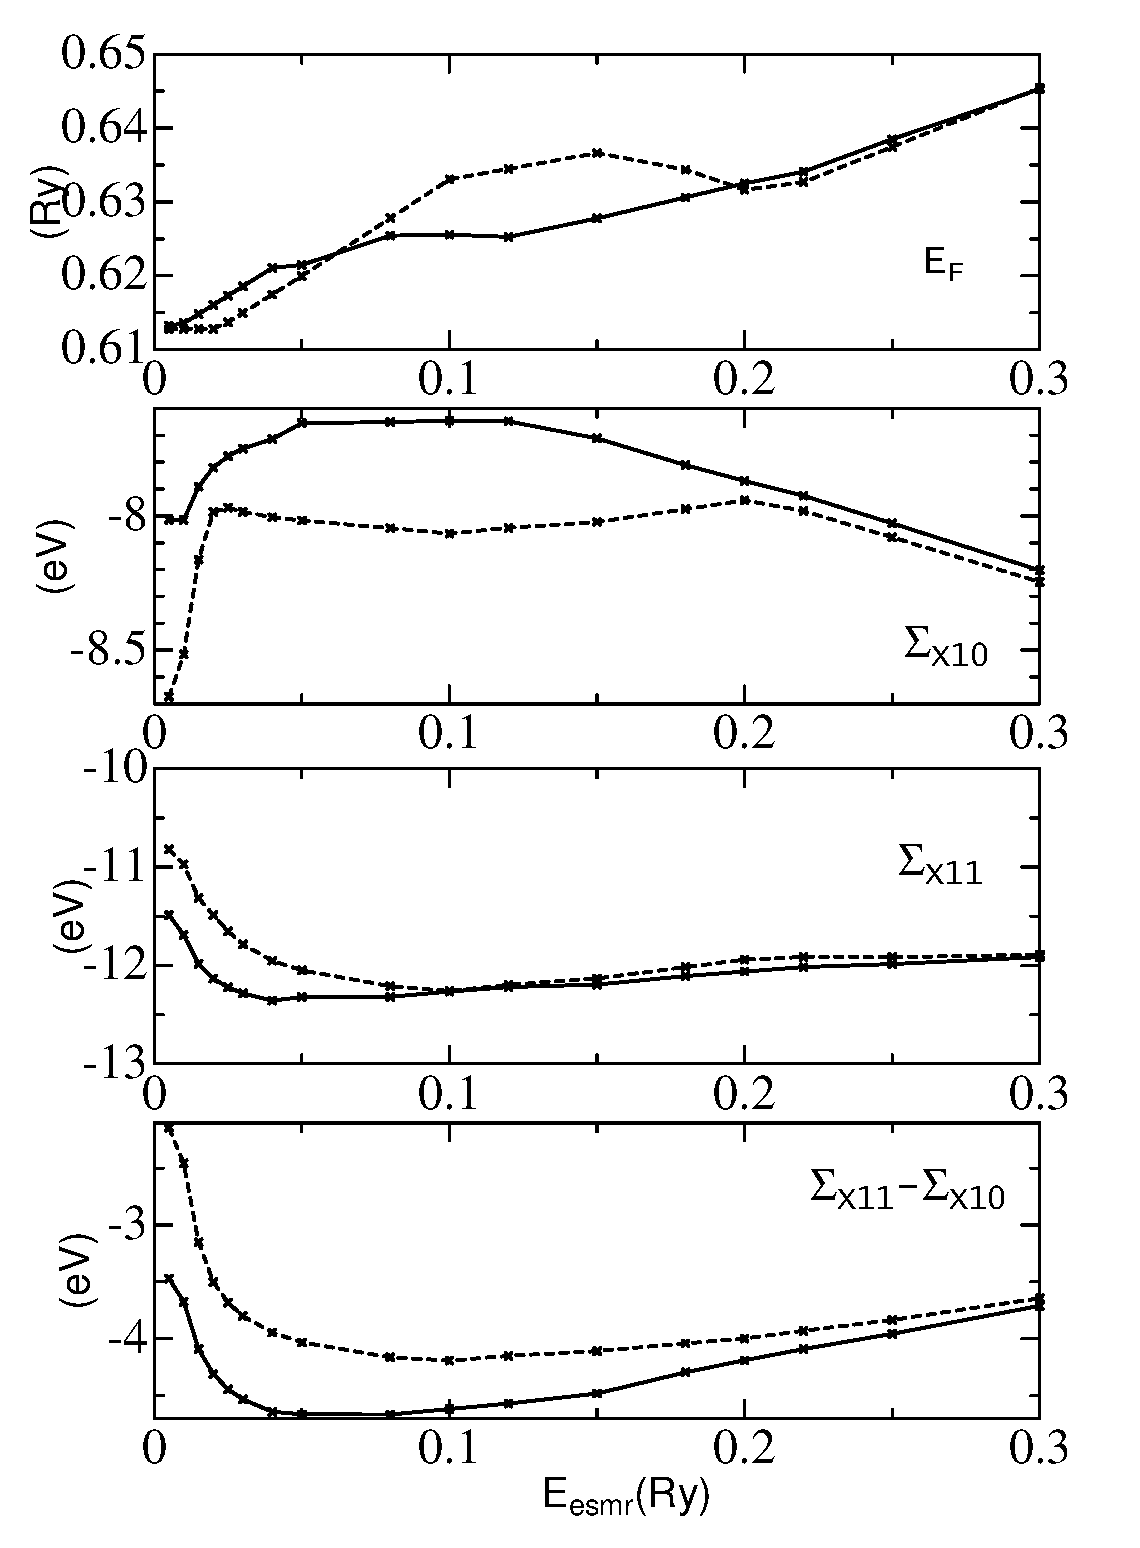
\includegraphics[width=15cm]{extest.eps}
\caption[]{$\langle \Psi_{{\bf q}n}|\Sigma_{\rm x} |\Psi_{{\bf q}n} \rangle$
as fucntions of $E_{\rm smear}$ for CaB$_6$, whose LDA bands are metallic.
({\tt GaussSmear}=off case).
The state $X_{10}$ is the top of the valence bands, and $X_{11}$ is the
bottom of the conduction bands. Solid line are for 666 case.
Broken lines are for 444 case. 
For ({\tt GaussSmear}=on), we expect somehow smoother behevior(not shown here). }
\label{extestcab6}
\end{figure}
\begin{figure}
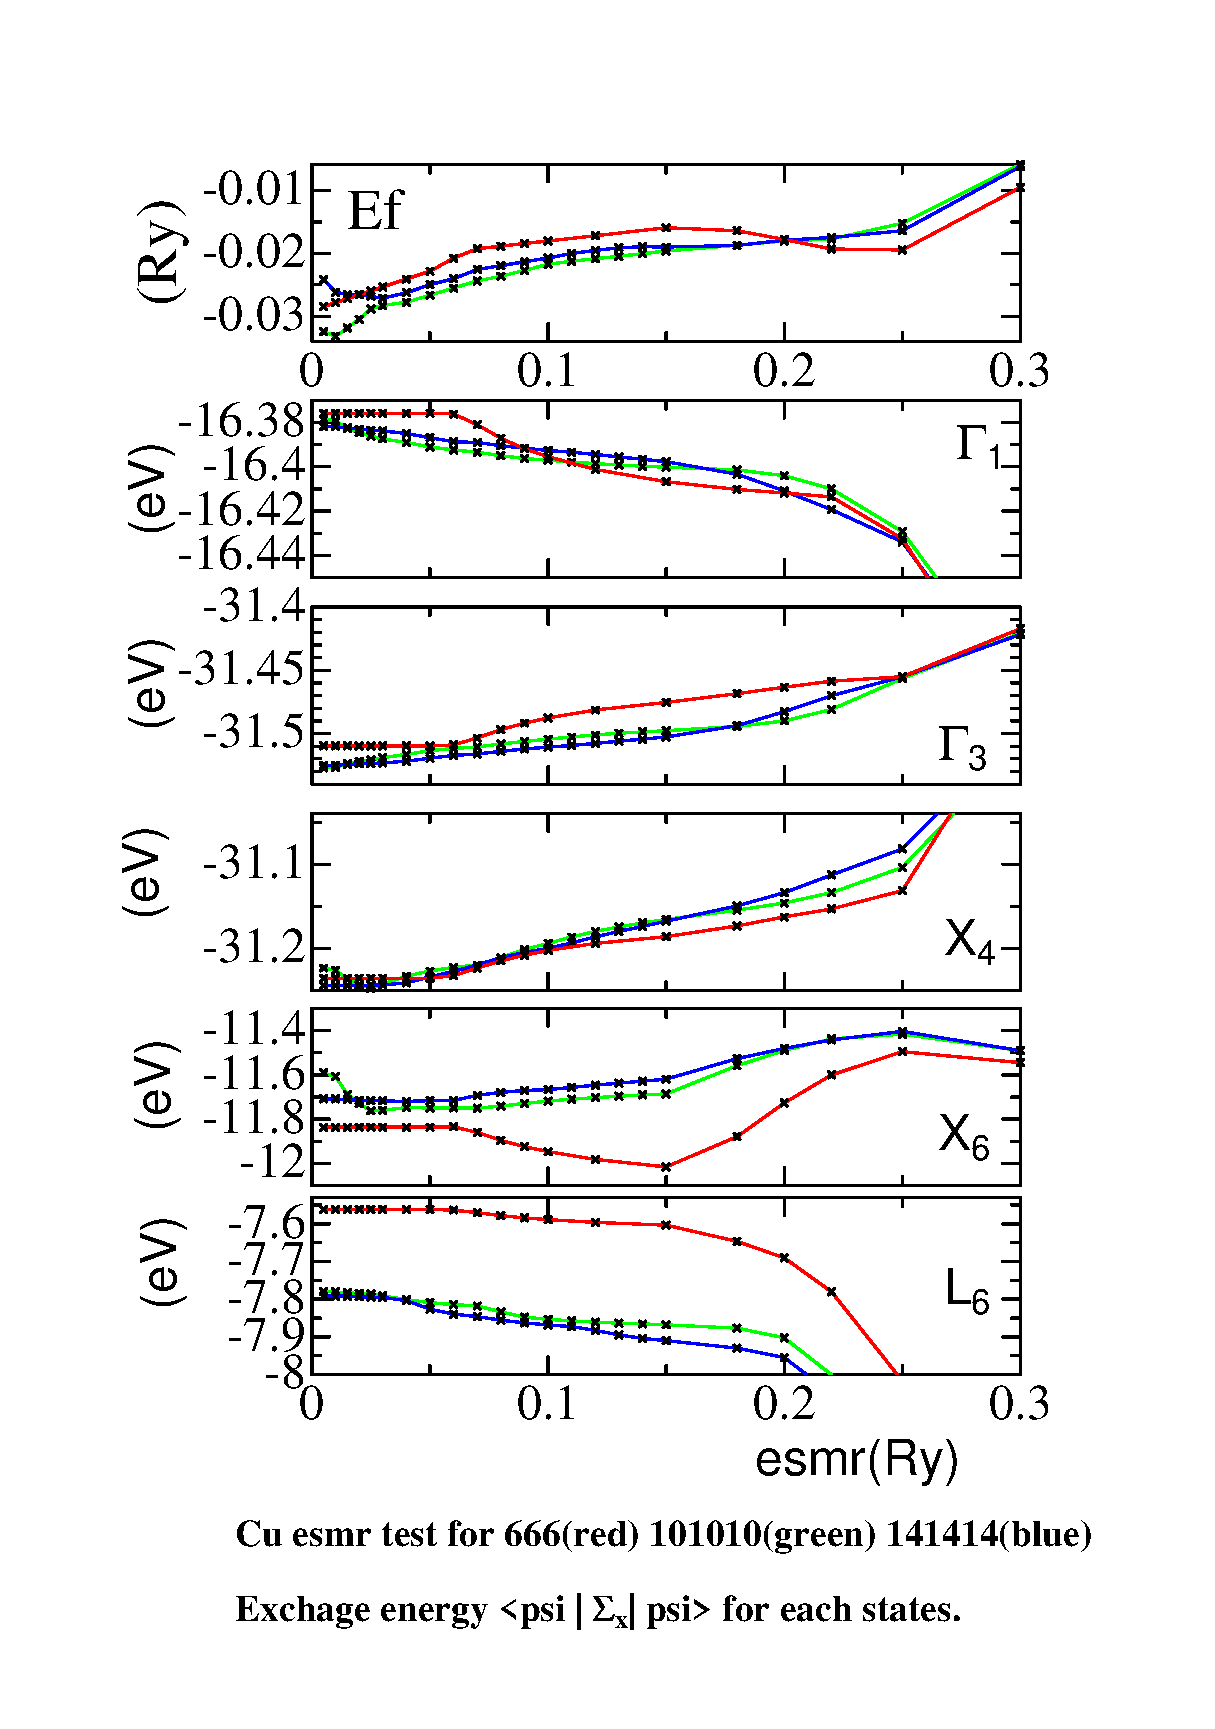
\includegraphics[width=15cm]{extest_cu.eps}
\caption[]{exchange self-energy test for Cu. ({\tt GaussSmear}=off case).
(esmr means $E_{\rm smear}$.) You can not use so small $E_{\rm smear}$ so as
to avoid the effects of discretization. We can use smaller $E_{\rm smear}$
for denser divisions(meshing) of BZ.
For ({\tt GaussSmear}=on), we expect somehow smoother behevior(not shown here). }
\label{extestcu}
\end{figure}


%%%%%%%%%%%%%%%%%%%%%%%%%%%%%%%%%%%%%%%%%%%%%%%%%%%%%%%%%%%%%%%%%%%%%
\newpage
\section{Package installation.}

\begin{enumerate}
\item
\verb#tar -zxvf fpgw033a1.tar.gz# in a directory ( at ecal/ or anythere else).
See fpgw/fpgw\_version\_log for changes from older versions.

\item
Move to fpgw/exec.  Modify \verb#fpgw/exec/make.inc#. Need BLAS and (a part of) LAPACK.

\item
Do \verb#make init#. This call a python script ``checkmodule'' and generate 
    moduledepends.inc, which is used for make.

\item
Do \verb#make#. This generates binaries. \verb#make install# just copy binaries to your bin
(set name of your bin in make.inc). \verb#make install2# copies scripts to your bin.

\item You also have to copy lmf lmfa lmfgw lmf2gw (these are from lmf(GW driver)) to your bin.

\end{enumerate}  

There are scripts---but most of all are for testing purpose. Important ones are\\
\verb#gw_lmfh#(one-shot \GW),\\
\verb#gwsc#(QSGW), \\
\verb#eps_lmfh, epsPP_lmfh# (epsion) ,\\
 \verb#epsPP_lmfh_chipm#(spin susceptibility).

 \

\noindent \underline{Test installation}. Copy fpgw/TESTinstallGW to another directory, and
do calculations (name of directory corresponds to the name of script;
e.g \verb#si:gw_lmfh# means 'do \verb#gw_lmfh si#'.
\begin{verbatim}
si:gw_lmfh/              Results: QPU 
si:gwsc/                        : QPU (you need to wait several itteration)
gas:gwsc/                       : QPU (you need to wait several itteration)
fe:eps_lmfh_chipm/              : ChiPM* 
fe:epsPP_lmfh_chipm/            : EPS*
gas:eps_lmfh/                   : EPS*
gas:epsPP_lmfh/                 : EPS*
\end{verbatim}
In each directory, you can do \verb#gw_lmfh# and so on.
Output of each srcipts are in \verb#out# file.
And results should be in agreement with QPU and so (as for gwsc case, agreement can be
not so perfect--- it depends of how to make convergence).
These tests may take minites to hours. \verb#si:gw_lmfh# requires a few minutes.





%%%%%%%%%%%%%%%%%%%%%%%%%%%%%%%%%%%%%%%%%%%%%%%%%%%%%%%%%%%%%%%%%%%%%
\newpage
\section{How to execute the \GW calculation? \ Overview.}

\ 

In this section, I will explain how to do the \underline{one-shot $GW$ calculation from LDA}.

\ 

\noindent----------------- Warning! --------------------------------------------------------
(probably I am sloppy about this rule).
\vspace{-5mm}
\begin{itemize}
\item
{\bf This font} is for executions or shell scripts.

\item
{\bf echo~3$|$hbasfp0 } means doing {\bf hbasfp0 } with the argument '3' from the standard input.
See the end of subsection \ref{mainstage}.

\item
{\sf This font} is for the I/O files by executions or by scripts.

\item
{\tt This font} is for files, directories, contents of files, or variables used in codes.

\item
\io{ctrl.si},\io{rst.si} and so on mean in the case of Si. 
You have to replace si with suitable name (extension of ctrl file).

\item
 There are files named {\sf {\it foo}U} and {\sf {\it foo}D}, which are
 for up spin and for down spin, respectively; e.g. ,{\sf SEXU} and {\sf SEXD}.
 We sometimes use {\sf {\it foo}U} to denote {\sf {\it foo}U} and {\sf {\it foo}D}.
\end{itemize}
\vspace{-5mm}
\noindent-----------------------------------------------------------------------------------

\ 

\noindent 

At first, you have to do the self-consistent FP-LMTO LDA calculation.
(It is done by \exe{lmfa} and \exe{lmf} in lm package.
Staring from \io{ctrl.si} (in the case of silicon),
you get the converged LDA potential in \io{rst.si}.) 
After you get the LDA result, you can start the \GW calculation
%\footnote{
%Mr.Usuda has developed the FP-LAPW based driver for \GW
%as a part of his Ph.D. work.}.
Practically, you have to follow steps below
in order to calculate the quesi-particle (QP) energies.

\vspace{3mm}

\begin{enumerate}
%\underline{\large Write \io{GWIN0} by hand.}
%
%{\sf GWIN0} contains primarily conditions of the \GW calculation.

\item[Step 1.]
\underline{\large Get LDA result.}
In lmf, you can start LDA calculation from \io{ctrl.si}
To start \GW, you need the LDA result \io{rst.si} together with \io{ctrl.si}.

[NOTE! Due to poorness of our \GW code, you have to use 
the same \verb#LMXA# ($l$ in the expansion of eigenfunction 
in each MT) for all the MT spheres.]

\item[Step 2.]
\underline{\large Run the script \exe{mkGWIN\_lmf2}.}

The purpose of this script is to get \io{GWinput.tmp}.
Other generated files are just useless (or for your info).

\item[Step 3.]
\underline{\large Edit \io{GWinput.tmp} and save it as \io{GWinput}}

These step 2. and step 3. are just only to get \io{GWinput}.

\io{GWinput} is the input file describing the computational 
conditions for \GW calculation. 


\item[Step 4.]
\underline{\large Run the script \exe{gw\_lmfh}.}

To invoke \exe{gw\_lmfh}, you needs files 
\io{ctrl.si}, \io{rst.si} and \io{GWinput} (in the case of si).
The main output are \io{QPU} files and so on; See Section \ref{mainoutput}.
If things OK, it shows as
\newpage
{\baselineskip=3mm
\begin{verbatim}
> gw_lmfh si
si
FORTRAN STOP  OK! qg4gw mode=1 normal mode
 OK! lmfgw mode=1 
FORTRAN STOP  OK! lmf2gw: end --- DATA4GW_V2 is written 
FORTRAN STOP  OK! rdata4gw_v2
FORTRAN STOP  OK! heftet mode=1 EFERMI generated 
FORTRAN STOP  OK! hchknw: write nw to NW
FORTRAN STOP  OK! hbasfp0 ix=3 core mode 
FORTRAN STOP  OK! hvccfp0 
FORTRAN STOP  OK! hsfp0: Core-exchange mode
FORTRAN STOP  OK! hbasfp0 ix=0 normal mode 
FORTRAN STOP  OK! hvccfp0 
FORTRAN STOP  OK! hsfp0: Sergey's Exchange mode
FORTRAN STOP  OK! hx0fp0 ixc=11 12 Sergey F. mode
FORTRAN STOP  OK! hsfp0: Sergey's Correlation mode
FORTRAN STOP  OK! hqpe 
\end{verbatim}
}
This output shows that the script {\bf gw\_lmfh} invokes {\bf lmfgw} and so on.
As we explain just below, the precedures until
"{\tt OK! lmf2gw: end --- DATA4GW\_V2 is written}" corresponds to the
end of {\bf (2)Preparation stage}.


\item[Step 5.]
\underline{\large Run the script {\bf hqpemetal} in the case of metal}

This is in order to get the correct Fermi energy by the tetrahedron method.

(To execute {\bf hqpemetal}, you need to calculate all the QP energies 
at least just above the Fermi energy).

[this is for old users: Note that the newer {\bf hqpemetal} will not work for old results by fpgw020;
you need to change \verb#nnv# in {\sf LMTO} file.]
\end{enumerate}

\vspace{2mm}

In the case of the Antiferro materials, the compuational efforts reduced to be half 
(only hx0fp0 part; most expensive for one-shot $GW$) if you prepare a file {\sf Anfcond} 
by handbefore you execute {\bf gw\_lmfh}. See next section for it.
(this function now works only for the case that 
a symmetry operation is [a translation verctor with spin inversion].)

\vspace{2mm}

%Unix shell scripts {\bf gw\_lmf} in the {\tt ecal/fpgw/exec} directory
%makes the procedure almost automatic.
%{\bf gw\_lmf} is for the \GW calculation including cores.
%{\bf gwnc\_{\it foo}} is for the \GW calculation without core.
%{\it foo} donotes the LDA method;we now have 
%implimented {\bf gw\_nfp}, {\bf gwnc\_nfp}, and {\bf gw\_lmf}.

From the view of computational procedure,
the \GW calculation are devided into these stages: \\
{\bf (0)LDA calculation }(step 1.)\\
{\bf (1)Pre-Preparation stage} (step 2-- step 3)\\
{\bf (2)Preparation stage} (step 4) \\
{\bf (3)Main stage} (step 4)\\
{\bf (4)Post Main stage} (step 5)\\
The script {\bf gw\_lmfh} automatically do all the procedures 
contained in the stage (3) and stage (4).

In anyway, it is necessary to look into these shell scripts, 
and observe the cosole outputs of each programs called from the script 
(they are usually reserved to \io{l*} files,e.g. \io{lbas} or so. 
Look into the scripts.) You don't need to understand all items in console outputs;
I am sloppy to orgainize it--- so, not so meanigful or debugging check write are 
in these console outputs.


\vspace{3mm}
\subsection{\bf (1)Pre-Preparation stage to write {\sf GWinput}}

The purpose of this stage is to write {\sf GWinput}.
So you can pass this stage if you have {\sf GWinput} already.
A template {\sf GWinput.tmp} is generated by \exe{mkGWIN\_lmf2}. 
Files used by \exe{mkGWIN\_lmf}2 are

\infiles

\fl{ctrl.si} The master control file of the self-consistent FP-LMTO LDA calculation.

\fl{rst.si}  This contains self-consistently-determined LDA potential.

\outfiles

\fl{GWinput.tmp} A file including computational conditions
for the \GW calculation.
In addition, it specifies the {\bf k} poins for 
which you calculate the QP energy.

\vspace{3mm}
When you invoke {\bf mkGWIN\_lmf}, 
it asks you to supply three numbers for BZ integration as
{\baselineskip=3mm
\begin{verbatim}
== Type three integers n1 n2 n3 for Brillouin Zone meshing for GW! ==
 n1= 
\end{verbatim}
}
Then you need to type a number e.g. as "2 \fbox{Return}" for n1.
Then you need to repeat it for n2 and n3 as\\
 n1= 2 \fbox{Return}\\
 n2= 2 \fbox{Return}\\
 n3= 2 \fbox{Return}\\
. 
These numbers specifies what k poins in BZ is used for BZ integration 
(In this case, $2\times 2\times 2=8$ {\bf k} point in the 1st BZ is used.
Based on our experiences, we need $4\times 4\times 4$ to get
band gap for Si with $\approx 0.1$ eV accuracy).

Then you have to edit {\sf GWinput.tmp} and copy it to
{\sf GWinput}. We details the {\sf GWinput} in later chapter.


\vspace{3mm}
\subsection{\bf (2)Preparation stage.}
In order to start this stage,
we need self-consistent LDA potential file and {\sf GWinput}.

\begin{itemize}
\item{\bf echo 0 $|$lmfgw}: 
  Get some small information files to start {\bf qg4gw}.
\item{\bf echo 1 $|$qg4gw }: Get ${\bf k}$ points used
  in the \GW calculations and the correponding ${\bf G}$ vectors.
\item{\bf echo 1 $|$lmfgw} : 
 Calculate the LDA eigenfunctions, eigenvlaues, and
 $\langle \psi | V^{\rm LDA}_{\rm xc}| \psi \rangle$
  for these ${\bf k}$ in the form of Eq.(\ref{psieq}).
\item{\bf lmf2gw}: store these datas into {\sf DATA4GW\_V2} and {\sf CphiGeig} , 
whose I/O is controlled by a key subroutine {\bf gwinput\_v2.f}.
\end{itemize}
\vspace{.3cm}
These procedures described in {\bf gw$\_$lmfh } are in the case fo FP-LMTO.

At the end of this stage, we get required eigenfunctions, BZmesh data, and so on,
which are required for the successive main stage.

{\small
\noindent ------note ------------------------------------------------\\
Here, e.g., {\bf echo 1$|$qg4gw} and so on means that we invoke {\bf qg4gw} with
the argument 1 from the standard I/O ( not from console).
So it is equivalent with

$>$qg4gw \fbox{Return}

$>$1 \fbox{Return}

from the console. 


But it may not go ahead if you still supply

$>$\verb|\| \fbox{Return}

in cases for {\bf hsfp0, hvccfp0, hx0fp0}, because they have two {\tt read(5,*)}
and you have to cause the readin error for the second read to go ahead
\footnote{The second read(5,*) is used for the case of parallel computing and
you need to cause the readin error for usual single machine computing;
(but this mode of pararallel computing is not maintained now).}\\
\noindent ------------------------------------------------------------------
}

\subsection{\bf (3)Main stage starting from {\sf DATA4GW\_V2}.}
\label{mainstage}
We can start the main stage of \GW cakckatuib from these files;

{\baselineskip=5mm

\fl{DATA4GW\_V2} Crystal structures and so.

\fl{CphiGeig} Eigenvalues and Eigenfunctions

\fl{QGpsi} q and G vector for the eigenfunction(q means {\bf k} in the previous section),

\fl{QGcou} q and G vector for the Coulomb matrix

\fl{Q0P}   q points near q=0 instead of q=0,

\fl{BZDATA} q points date (and tetrahedron weights if necessary) for BZ integrals.

\fl{QIBZ}  irreducible q points (This is also contained in {\sf BZDATA}).

\fl{CLASS} class information for atomic sites.

\fl{SYMOPS} point group operation

\fl{GWinput} computational conditions.

\noindent These files are not dependent on how to prepare 
the eigenfunctions, whether LMTO or LAPW.
If you want to do GW calculation with eigenfunction given by other codes,
you have to write "a $GW$ driver routine" which generates
files {\sf DATA4GW\_V2}, {\sf CphiGeig} and {\sf CLASS} by yourself.
(See later sections for these files).

As for the computational flow of the procedure,
see the script {\bf gw$\_$lmfh}. As for this stage, {\bf gw$\_$lmfh} do;

\begin{itemize}
\item{\bf rdata4gw\_V2}: 
  Read {\sf DATA4GW\_V2}, and decompose it into files required in
  the followings. 
\item{\bf heftet   }: Get the Fermi energy {\sf EFERMI} by tetrahedron method. It is used in {\bf hx0fp0}.
\item{\bf hchknw   }: stores the number of required $\omega$ points along real-axis into {\sf NW}. \\
{\small ({\sf NW} is not essentially used, but is supposed to exist in the followings.)}
\item{\bf echo 3$|$hbasfp0}: gives the product basis for Core exchange.
\item{\bf echo 0$|$hvccfp0}: gives the Coulomb matrix for the Core exchange.
\item{\bf echo 3$|$hsfp0  }: gives the Core exchange part of the self-energy.
\item{\bf echo 0$|$hbasfp0}: gives the product basis.
\item{\bf echo 0$|$hvccfp0}: gives the Coulomb matrix $v$.
\item{\bf echo 1$|$hsfp0  }: gives the exchange part of the self-energy.
\item{\bf echo 1$|$hx0fp0 }: gives the correlated part of the screened Coulomb interaction $W-v$.
\item{\bf echo 2$|$hsfp0  }: gives the correlated part of the self-energy.
\item{\bf echo 0$|$hqpe   }: gather datas and write down final results into {\sf QPU} and so on.
\end{itemize}
\vspace{.3cm}

Then you can do the script {\bf hqpemetal} in the case of metal in order to get
the Fermi energy for the QP energies.


\vspace{3mm}
\subsection{\bf Other functions (or scripsts)}
In addition to {\bf gw\_lmfh}, there are some other additional scripts 
and functions.

\begin{itemize}
\item
{\bf gw\_lmfh} : The one-shot \GW calculation explained here. \\

\item
{\bf gwsc} : Semi self-consistent \GW calculation.

\item
{\bf \ epsPP\_lmfh, eps\_lmfh} : Dielectric function without or with local-field effects.

\item
 run-mode 4 of {\bf hsfp0}: to plot the spectrum function $\Sigma(\omega)$. 

\item
{\bf gwband\_lmf} : for plotting band (not well maintained now).

\item
{\bf epsPP\_lmfh\_chipm} : non-interacting spin susceptibility. 
One-degree of freedom like Rigid moment approx.
After it ends, you need to do \verb#calj_nlfc_metal# and/or \verb#calj_summary_mat#
to get the full spin susceptibility.

\end{itemize}

 \

Scripts below are for tests 
\begin{itemize}
\item
{\bf extest, \ extest\_repeat}: 
which is in order to check the dependence of $\Sigma_{\rm x}$ as for $E_{\rm smear}$.

{\bf gw\_lmf} : The one-shot \GW calculation, older version. \\
(Direct calculation of the polarization function
without going through the Hilbert-transformation.

\item
{\bf \ eps\_lmf}   : Dielectric function with local-field effects. 
Direct mode(Not Hilbert-transformation).

\item
{\bf gwpara\_lmf} : A test gw script for parallel computing (testing. it may not work now).

\item
{\bf eps\_lmfh\_chipm} : spin susceptibility (full mixed basis). Test purpose.
\end{itemize}


\newpage
\section{GWinput}
\label{maininput}

The main input files is {\sf GWinput}.
[it is a unified file of old {\sf GWIN0},  {\sf GWIN\_V2}, and {\sf QPNT}].
This controls the setting of \GW calculation.
The file {\sf GWinput} consists of
structures as\\
{\it keyword1 data1}\\
{\it keyword2 data2}\\
...\\
In each lines, it consists of keyword and data. 
Data can be sigle or plural.
As for keywords, upper case or Lowercase is not distingushed.
All keywords should start from 1st column (no space at head).
Order of lines are irrelevant.
As for logical variable, you can use 
anything among (true, ok, .true. yes, on, 1, T) for .true.,
and anything among (false, ng, .false., no, off, 0, F) for .false.\\

Or we have ``tag sections'' in {\sf GWinput} 
specified by \verb#<PRODUCT_BASIS>#, 
\verb#<QPNT>#,  \verb#<PBASMAX>#, \verb#<QforEPS>#, and \verb#<QforEPSL>#.
(\verb#<PRODUCT_BASIS># is requires for all kinds of calculations.
\verb#<PBASMAX># is optional. \verb#<QforEPS># and/or \verb#<QforEPSL># are required
for eps mode). It is like
\begin{verbatim}
<PRODUCT_BASIS>
 tolerance to remove products
  0.100000D-07 ! =tolopt
 lcutmx(atom) 
  3 3 
  atom   l
...
</PRODUCT_BASIS>
\end{verbatim}
. In these tag sections, you have to keep format for its own
(usually numbers are readin by free format \verb#read(5,*)#).

The fundamental readin routine for \GWinput is a subroutine 
\verb#getkeyvalue# defined in \verb#gwsrc/keyvalue.f# written by Dr.Kino.
\verb#getkeyvalue# is a general and convenient readin routine in full use of the f90 features.
Read a head part of the file and try to do "grep getkeyvalue *.F" 
in \verb#gwsrc/# or \verb#main/# so as to see how to use it
(test routine is \verb#main/kino_input_test.F#.)

So the {\sf GWinput} consists of three sections \\
1.General section \\
2.\verb#<PRODUCT_BASIS># section\\
3.\verb#<QPNT># section\\
4.\verb#<PBASMAX># section\\
5.\verb#<QforEPS>#,\verb#<QforEPSL># section\\
We will explain each by each in the followings.

%%%%%%%%%%%%%%%%%%%%%%%%%%%%%%%%%%%%%%%%%%%%%%%%%%%%%%%%%
\newpage
\fx{General section}

In genral section, it looks like

\begin{verbatim}
! ##### From GWIN0 ################ 
n1n2n3  2 2 2   ! for BZ meshing in GW 
QpGcut_psi  2.7 !(See unit_2pioa for unit) |q+G| cutoff for eigenfunction.
QpGcut_cou  2.5 !(See unit_2pioa for unit) |q+G| cutoff for Coulomb and W.
unit_2pioa  off ! on--> unit of QpGcut_* are in 2*pi/alat; off --> a.u.
emax_chi0   4.  !(Ry) emax cutoff for chi0  (Optional)
emax_sigm   2.  !(Ry) emax cutoff for Sigma (Optional)

alpha_OffG  1   !(a.u.) Used in auxially function in the offset-Gamma method.

! ##### FREQUENCIES from GWIN_V2 ################ 
dw      0.01  !(a.u.) mesh width along real axis.
omg_c   0.05  !(a.u.) Only meaningful for Sergey mode as gw_lmfh.
              ! coaser mesh for higher energy. Width get to be doubled at omg_c.
niw        6  ! Number of frequencies along Im axis. Used for integration to get Sigma_c
              ! E.g. try niw=6 and niw=12
delta -.1D-7  !(a.u.)  Broadening of x0. negative means tetrahedron method.
              ! used by hx0fp0. You get smeard x0 witth abs(delta).
deltaw 0.020  !(a.u.)   Mesh for numerical derivative to get the Z factor
GaussSmear on ! Gaussian or Rectangular smearing for Pole of G^LDA with esmr for hsfp0.
esmr   0.003  !(Ry) used by hsfp0. Keep esmr smaller than band gap for insulators
              ! Poles of G^LDA are treated as if they have width esmr in hsfp0. 
              ! Change esmr for metals.  See DOSACC*---especailly around Ef.
\end{verbatim}

---------------------------------------------------\\
\begin{enumerate}
\item 
\keyw{n1n2n3} 3 integers as $N_1,N_2,N3$ (no default); They are $\ge 0$. \\
Brillouin Zone mesh for integeration
is determined by keywords{\tt BZmesh} and {\tt n1n2n3}. 
In EQS.47(regular mesh) or 53(off-regular mesh).\\

\keyw{Chi\_RegQbz} (on or off)

     Chi\_RegQbz = on (default): Use regular mesh (including gamma) for eps calculation.

     Chi\_RegQbz = off         : Use off-regular mesh (Not including gamma) for eps calculation.

\keyw{BZmesh} (1 or 2)

     BZmesh 1(default) : Use regular mesh (including gamma) for sigma calculation.

     BZmesh 2          : Use off-regular mesh (Not including gamma) for eps calculation.

     So we now have four (2x2) combinations for the 1shot GW calculation
     (Chi\_RegQbz x BZmesh). 
     I think that BZmesh 2 is now not good for self-consistent GW.

\item 
Plane wave (${\bf q+G}$) cutoff  \\
\keyw{QpGcut\_psi} 1 real (no default)\\
\keyw{QpGcut\_Cou} 1 real (no default)\\
\keyw{unit\_2pioa} 1 logical (no defalt)\\
We have two cuoff for ${\bf q+G}$.
{\tt QpGcut\_psi} is the cutoff of $|q+G|$ for the IPW 
in the expansion of the eigenfunctions.
{\tt QpGcut\_Cou} is for the IPW of the interactions $v,D,W$.
Its unit is specified by {\tt unit\_2pioa };
"off" means unit in a.u. and "on" means in unit of $\frac{2 \pi}{\mbox{\rm alat}}$.
(alat is length scale unit in {\sf ctrl.*}).


\item 
Cutoff for used bands.\\
\keyw{emax\_chi0}: 1 real (optional,default=$\infty$), in Ry\\
\keyw{emax\_sigm}: 1 real (optional,default=$\infty$), in Ry\\
\keyw{nband\_chi0}: 1 integer (optional,default=$\infty$)\\
\keyw{nband\_sigm}: 1 integer (optional,default=$\infty$)\\
These specify how many bands you use in {\bf hx0fp0} (for chi0) 
and in {\bf hsfp0} (for sigma). 
Higher bands above them are neglected.

\item 
Energy mesh related parameters.\\
\keyw{dw}     : 1 real (a.u.). Mesh width along real axis for $W(\omega)$.\\
\keyw{omg\_c} : 1 real (a.u.). \\
{\tt dw} and {\tt omg\_c}
determines $\omega$ mesh along real axis for $W(\omega)$.
Energy mesh is getting coarser at higher energy. 
Energy bin width get to be doubled at {\tt omg\_c}.\\
But {\tt omg\_c} is not used in gw\_lmf; then energy mesh is fixed as {\tt dw}.
We calculate $W(\omega)$ at these energy mesh as 
$W(\omega=0), W(\omega={\tt dw}), W(\omega=2 \times {\tt dw}), W(\omega=3 \times {\tt dw}), ...$
and then use them for the numerically interpolate 
to determine $W(\omega'=\omega-\epsilon_{{\bf q-k}n})$. See FIG.1 in Ref.I.

\underline{(WARNING! Some of my examples may show as if they are in "(Ry)". But they are Wrong!)}\\

\vspace{2mm}
\keyw{delta} : 1 real (a.u.). Fix it as -1d-8 or so for gw\_lmfh, eps mode and so.
This is the size of $\delta$ in denominator of $\Pi$ (EQ.32).
But (I think that) you can not use it so as to make broadning 
for theoretical test (maybe not exactly corresponding to $\delta$).\\

[Old note. Need check:
In gw\_lmf, it is used for broadening of x0 when it call hx0fp0.
Then {\tt delta} is $\delta$ is EQ.32.
The sign of {\tt delta} is just used as a flag whether you use the
tetrahedron method of dielectric constant \cite{rath75} or not; minus sign means
"Use the tetrahedron method for $D$"; plus sign means you do it by simple sum.
You can usually use this default setting. But it might be possible
to use a larger value to smear the fine structures
on the energy-dependence of $W$ in cases.
This might be necesary if $W$ is so energy-dependent 
and \verb#dw# is not so small to resolve the structure
---but I don't know.]\\


\keyw{niw} : 1 integer. \\
Number of integration points along the imaginary axis(FIG.1)
to get $\Sigma_c$.
See routines {\tt wint*} called from {\tt sxcf*.F},
which is called from the main routine {\tt hsfp0.m.F} (or {\tt hsfp0.sc.m.F} in the QSGW case).
The integration points are
$i \omega'(n)= i( 1/x(n) -1)$, where $x(n)$ is
the usual Gaussian-integration points for the interval [0,1].
In addtion, we give the special analitical treatment for
the peakey part at $\omega'=0$.
Out tests shows {\tt niw}=6 for Si is good enough for 0.01 eV accuracy.
The convergence as for {\tt niw} is quite good.
This integration scheme has been devloped by Ferdi Aryasetiawan.
The number of points should be the one of 6,10,12,16,20,24,32,40,or 48. 
It is because we use a {\tt subroutine gauss} in {\tt /gwsrc/mate.F} 
prepared by Ferdi. We will replace better one in future.
See II-F in Ref.I.\\

\keyw{GaussSmear} : 1 logical \\
\keyw{esmr} : 1 real (Ry). Used by hsfp0 (and hsfp0.sc for QSGW). \\
Poles of  the Green fucntion $G^{\rm LDA}$ are treated as if they have width esmr in hsfp0. 
If {\tt GaussSmear} is on, each pole of $G^{\rm LDA}$
is smeared by a Gaussian function with $\sigma=${\tt esmr} in the calculation of hsfp0.
If {\tt GaussSmear} is off, we assume rectangular smearing for the poles.
Usually it is necessary to take rather smaller value than band gap 
for insulators. Try to use 0.003 or so in the case of Si and {\tt GaussSmear}=on.\\
In the case of insulator, it can be smaller 0.0001 or less (maybe), 
but it should have some size in the case of metal.

\keyw{deltaw}: 1 real (a.u.) only for one-shot case.

{\tt deltaw} is the interval for the numerical derivative
$\frac{\partial \Sigma(\omega)}{\partial \omega}$ in EQ.8.
We calculate $\langle \psi^{{\bf k}n} |\Sigma(\epsilon^{{\bf k}n}+{\tt deltaw}) |\psi^{{\bf k}n} \rangle$ 
and $\langle \psi^{{\bf k}n} |\Sigma(\psi^{{\bf k}n}\!-\!{\tt deltaw})|\psi^{{\bf k}n} \rangle$
in addition to $\langle \psi^{{\bf k}n} |\Sigma(\epsilon^{{\bf k}n})|\psi^{{\bf k}n} \rangle$.
From these values, we can calcuate two $Z$ (or second-derivative of $\Sigma(\omega)$), as shown
in {\sf SECU}. It will help to see whether the used \verb#deltaw# is O.K. or not.

\item Offset-gamma point.\\
\keyw{Q0P\_Choice 0}:1 integer\\
{\tt Q0P\_Choice} gives how to determine the offset gamma points.
Initially we take them as\\
0: 6 points along plat.(default)\\
1: 6 points along along Ex Ey Ez. \\
2: 4 points in plat(1:3,1),plat(1:3,2)\\
3: 2 points in plat(1:3,3)\\
Then we choose only inequivalent ${\bf q}$ points
based on the point group symmetry.
We found {\tt Q0P\_Choice 0}=3 together with BZmesh=2 
works for 1 dimentional atomic chain along z-axis. 
See q0irre.f and search Q0Pchoice().
Obtained offset gamma points is given in a file {\tt Q0P}.

\keyw{alpha\_offG}: 1 real (a.u.) \\
{\tt alpha\_offG} corresponds to $\alpha$ in EQ.48.
{\tt alpha\_offG}=1d0 is usually good in the sense that
it seems to be almost a limit at $\alpha \to 0$.
So you can usually fix it as {\tt alpha\_offG}=1d0, and check the
convergence as for {\tt n1n2n3}.


\keyw{WgtQ0p } 1 real (in a.u.) (default=0.01). effective only for BZmesh=2\\
{\tt WgtQ0p} is the total weight for the offset gamma 
in the case of {\tt BZmesh}=2
(it is the ratio to the weight for regular mesh point as 1/(n1*n2*n3).).
It is usually OK to take 0.01 (default).
In principle, the final result should not depend on {\tt WgtQ0p}.
We observed that QPE changes little from {\tt WgtQ0p}=0.01 through 1d-6 in cases.
(For rather small {\tt WgtQ0p}, you have to care that the normalization of eigenfunction is 
good enough. In order to make the normalization better(see file normchk.dia), 
you have to use larger {\tt QpGcut\_psi}.). \\

Note:In addition, we found that it was necessary to use \verb#LMXA=6#
($l$ in the expantion of eigenfunction in MT) or so was necessary
to keep the normarization of eigenfunction rather accurately for Na.

\item core orthogonalization (default=off)\\\\
\keyw{CoreOrth} 1 logical\\
If this is on, we enforce cores orthogonalied to valence 
$\phi$ and $\dot{\phi}$ (these appear in II-C in Ref.I).
This procedure enforce the correct orthogonal condition, thus
we have correct behevior for the dielectric function at ${\bf q} \to 0$.
However, it may deform core functions too much, 
especially in the case of shallow 3d (or maybe 4d) cores.
So we don't recoommend make it on usually, even though then 
the orthogonality condition is somehow broken.
Anyway you can check wether it affects to results or not by this switch.


\item QP self-consistent GW.\\
\keyw{iSigMode} 1 integer (nodefault).\\
This is required for semi self-consistent GW calculation by a script {\bf gwsc}.

1:\ Use $\ds \Sigma_{nn'}(E_F) + \delta_{nn'}(\Sigma_{nn'}(\epsilon_n)-\Sigma_{nn'}(E_F))$
   (EQ.11 mode-B).

3:\ Use $\ds {\rm Re}\frac{\Sigma_{nn'}(\epsilon_n)+\Sigma_{nn'}(\epsilon_{n'})}{2}$
  (EQ.10 mode-A).

5:\ Use $\ds \delta_{nn'} \Sigma_{nn}(\epsilon_n)$ (Eigenvalue-only self-consistency).

See \verb#/gwsrc/sxcf_fal2.sc.F#.
In order to do QS\GW by {\bf gwsc}, you have to set some options
in {\tt ctrl.*} so that {\bf lmf} can read the generated $\Sigma$ by my GW code (sigm file).
It is detailed in the $GW$ driver manual in Mark's lmf, and also see Section \ref{scgw}.

\item Others\\
\keyw{KeepEigen} 1 logical (default=on)\\
\keyw{KeepPPOVL} 1 logical (default=on)\\
These are for memory usage.
If KeepEigen is on, eigenfunctions (Eigen) are kept in memory during calculation.
If KeepPPOVL is on, the overlapping mamtrix (PPOVL) is stored 
in a memory. If you have not enough memory in your machine,
use them off. Then you can save memory usage.
However, then we have too frequent accsess to files.
So \%CPU might get lower. Be careful to use these options.


\keyw{Verbose} 1 integer (default=0)
If 0, it gives minimum standard output.
If 40 or higher, it shows too much output.
(these verbosity control is not well-organized yet). 

\keyw{multitet} 3 intgers. (optional) Now only "2 2 2" is allowed.\\
If you set "{\tt multitet  2 2 2}", 
it affects hx0fp0 (to calculate the polarization function $\Pi$) 
thought the tetrahedron weights.
When we set this, each tetrahedron is further devided into $2\times 2\times2=8$ 
micro tetrahedrons. Weights from the tetrahedron are calculted
as the sum of contributions from these micro tetrahedrons,
where we utilize eigenvalues at corners of these micro tetrahedron.

In other words, this is a technique to include changes of eigenvalues
though BZ efficiently under the assumption 
that the behevior of eigenfunctions are rather smooth.

However, we found this is not so efficient.
So we don't recommend to set this option.

\end{enumerate}



%%%%%%%%%%%%%%%%%%%%%%%%%%%%%%%%%%%%%%%%%%%%%%%%%%%%%%%%%%%
\newpage
\fx{$<$QPNT$>$ section} 
This section is to specify the q points and bands index for which you calculate 
the QP energies (QPE). An example is
{\baselineskip=2.6mm
\begin{verbatim}
<QPNT>
 --- Specify the q and band indeces,  for which we evaluate the self-energy ---

*** all q -->1, otherwise 0;  up only -->1, otherwise 0
           0           0
*** no. states and band index for calculation.
          3
  15 16 17 
*** q-points, which shoud be in qbz.  See KPNTin1BZ.
           2
  1     0.0000000000000000     0.0000000000000000     0.0000000000000000
  2     0.2886751358562925    -0.5000000000000000     0.0000000000000000
  3     0.0000000000000000     0.0000000000000000     0.3073140749846343
</QPNT>
\end{verbatim}}
Numbers are read by free format read(5,*), 
thus the numbers should be separeted by space.
At the next line to the first {\tt ***},
you have to give two numbers used as flags. 
Both of them takes 0 or 1.
1st one is whether you calculate QPE for all q points (in IBZ) or not.
If it is 1, you calculate  QPE for all q. If it is 0, you calculate them only for
q points specified within this file. In the case of metal where you want to calculate the Fermi energy for QPE,
you need to calculate all the eigenvalues somehow above the Fermi energy
(If you put 1, it is safer but too time-consuming).
The second number is whether you calculate QPE for
both spins or not. 
It is usually 0. In the case of antiferro material, 
it should be 1.

From the next line to the second {\tt ***},
you have to specify the states for which you calculate teh QPE.
In this example, you calculate the 3 bands of QPE for
15th, 16th, and 17th eigenfunctions 
(they are ordered from the bottom).

From the next line to the third {\tt ***},
you have to specify the q points. 
The first numbers of each line are dummy.
In this case, you calcualte QPE for two q points.
The third q point is neglected because 2 is given at first.

When you generate GWinput.tmp, you see all the possible $q$ points 
are listed (these q points should be a part of the regular mesh points).

In the QS\GW mode (gwsc),
this section is neglected (then we calculate all QPE on regular mesh points); 
so its hsfp0\_sc part is quite expensive (usually it takes time more than hx0fp0).

 \

\noindent Additional Note --------------\\

\noindent \keyw{QPNT\_nbandrange} num1 num2 (two integers).\\
This overide setting in \verb#<QPNT>#. (I think this switch still works).\\

\noindent \keyw{AnyQ} on (default is off)\\
If this is on, you can spefify any Q point which is not on the mesh point.
For the purpose, we need to prepare eigenfunctions at extra $\bf k$ points.
But it is automatic. In order to make the computaiton efficient.
Even in this case, from the computational view, it is better to choose
${\bf q}$ on the two times finer devided mesh (or three times finer devided ${\bf k}$ mesh).
This is used for Fig.6 in Phys. Rev. B 74, 245125 (2006).


%%%%%%%%%%%%%%%%%%%%%%%%%%%%%%%%%%%%%%%%%%%%%%%%%%%%%%%%%%% 
\newpage
\fx{set QPNT for eps mode} 
For eps modes (scripts \verb#eps_*#, which are for linear responses. See Sec.\ref{linearr}),
you have to specify q point in the following ways.\\

\noindent 1. \keyw{QforEPSIBZ} on\\
Then all Q point in IBZ are used.\\

\noindent 2. Use section as
\begin{verbatim}
<QforEPS>
0d0 0d0 0.01d0
0d0 0d0 0.02d0
0d0 0d0 0.04d0
0d0 0d0 0.08d0
</QforEPS>
\end{verbatim}
In addition, you can specify Q points as
\begin{verbatim}
<QforEPSL>
0d0 0d0 0d0   1d0   0d0  0d0 8
0d0 0d0 0d0  .5d0  .5d0  0d0 8
</QforEPSL>
\end{verbatim}
This is along the line--- 8 point along the line (not left-end q; so omitting 0 0 0).
The first line means line (0d0 0d0 0d0)---(1d0 0d0 0d0) is devided to 8. 
So we have 7 points, (0.125 0 0), (0.25 0 0),... (1 0 0).



%%%%%%%%%%%%%%%%%%%%%%%%%%%%%%%%%%%%%%%%%%%%%%%%%%%%%%%%%%%
\newpage
\fx{$<$PRODUCT\_BASIS$>$ section} 
This section is to define product basis to expand $W$ and so.
Numbers are read by free format read(5,*),thus the numbers should be separeted by space.
The line number in this section is meaningful (you can not add comment lines).
{\baselineskip=2.6mm
\begin{verbatim}
<PRODUCT_BASIS>
 tolerance to remove products due to poor linear-independency
  0.100000D-04 ! =tolopt; larger gives smaller num. of product basis. See lbas and lbasC, which are output of hbasfp0.
 lcutmx(atom) = maximum l-cutoff for the product basis.  =4 is required for atoms with valence d, like Ni Ga
  4  3
  atom   l  nnvv  nnc ! nnvv: num. of radial functions (valence) on the augmentation-waves, nnc: num. for core.
    1    0    2    3
    1    1    2    2
    1    2    3    0
    1    3    2    0
    1    4    2    0
    2    0    2    1
    2    1    2    0
    2    2    2    0
    2    3    2    0
    2    4    2    0
  atom   l    n  occ unocc  ! Valence(1=yes,0=no) 
    1    0    1    1    1   ! 4S_p  ----- 
    1    0    2    1    0   ! 4S_d        
    1    1    1    1    1   ! 4P_p        
    1    1    2    0    0   ! 4P_d        
    1    2    1    1    1   ! 4D_p        
    1    2    2    0    0   ! 4D_d        
    1    2    3    1    1   ! 3D_l        
    1    3    1    0    1   ! 4f_p        
    1    3    2    0    0   ! 4f_d        
    1    4    1    0    0   ! 5g_p        
    1    4    2    0    0   ! 5g_d        
    2    0    1    1    1   ! 2S_p  ----- 
    2    0    2    0    0   ! 2S_d        
    2    1    1    1    1   ! 2P_p        
    2    1    2    0    0   ! 2P_d        
    2    2    1    1    1   ! 3d_p        
    2    2    2    0    0   ! 3d_d        
    2    3    1    0    1   ! 4f_p        
    2    3    2    0    0   ! 4f_d        
    2    4    1    0    0   ! 5g_p        
    2    4    2    0    0   ! 5g_d        
  atom   l    n  occ unocc  ForX0 ForSxc ! Core (1=yes, 0=no)
    1    0    1    0    0      0    0    ! 1S -----
    1    0    2    0    0      0    0    ! 2S      
    1    0    3    0    0      0    0    ! 3S      
    1    1    1    0    0      0    0    ! 2P      
    1    1    2    0    0      0    0    ! 3P      
    2    0    1    0    0      0    0    ! 1S -----
</PRODUCT_BASIS>
\end{verbatim}}

\vspace{5mm}
\noindent $\bullet$ This section is read in the free format in fortran.
So, e.g., \verb#0.01# works as same as \verb#0.10000D-01#.
The line order is important 
(you have to keep the order given by \io{GWinput.tmp}).
Be careful atom atom id---lmf may re-order it and pass it to gw code.
Look into LMTO file (generated by {\bf mkGWIN\_lmf2}); 
which contains crystal structure information after such re-ordering by lmf.
I used \verb#!# to make  clear that things after \verb#!#
are comments. But \verb#!# is not meaningful -- just the expected
numbers of datas separeted by blank(s) are read for each line 
from the begining of lines.


\vspace{5mm}
\noindent $\bullet$ The real number in second line \raw{tolerance} is
to remove the poorly linear-independent product basis.
If multiple numbers are specified, it means \raw{tolerance} for each atoms.

You can also use \verb#<PBASMAX># section to override this setting. It is given as
\begin{verbatim}
<PBASMAX>
1  5 5 5 3 3
2  5 5 3 2 3
3  3 3 2 2 2
</PBASMAX>
\end{verbatim}
The first numebr is for atom index (fixed), and other are product basis 
for each $l$ channel.


\vspace{5mm}
\noindent $\bullet$ The integer numbers in 4th line \raw{lcutmx}
gives the maximum angular momentum $l$ for the procduct basis
for each atomic site.
In our experience, \raw{lcutmx}=4 is required
when the semi-core (or valence ) $3d$ electons exist
and we want to calculate the QP energies of them.

\vspace{5mm}
\noindent $\bullet$ Keep a block starting from 
"  atom   l  nnvv  nnc ..."  as it originally generated 
in \io{GWinput.tmp}. It just shows that how many kinds of radial functions
for cores and valence electrons for ecah atom and l.
{\tt nnvv}=2 in the case of $\phi$ and $\dot{\phi}$;
{\tt nnvv}=3 in the case to add the local orbital in addition.

\vspace{5mm}
\noindent $\bullet$ There are two blocks after the line
"{\tt   atom   l    n  occ  unocc  :Valence(1=yes, 0=no)}'
and after
"{\tt   atom   l    n  occ unocc  ForX0 ForSxc ! Core (1=yes, 0=no)}'.
These are used to choose atomic basis to construct the product basis.
The product basis are generated from the products of two atomic basis.

{\sf GWinput.tmp} generated by {\bf mkGWIN\_lmf2} contains
labels on each orbitals as \verb#4S_p#, \verb#4S_d#, \verb#4P_p#...
Here \verb#4S_p# is for $\phi_{4s}$; \verb#4S_d# for $\dot{\phi}_{4s}$;
\verb#3D_l# for $\phi^{\rm local}_{3d}$. 
Capital letter just after the principle-quantum number
means the orbital is used as `Head of MTO'; lowercase means just used only 
as the `tail of MTO'.

The swithces for columns labeled as \verb#occ# and \verb#unocc#. take 0 (not included) 
or 1 (inclueded). With the switch, we can construct two groups of orbitals,
\verb#occ# and \verb#unocc#.
In this sample {\sf GWIN\_V2} as for atom 1,
$\{ \phi_{4s},\dot{\phi}_{4s},\phi_{4p},\phi_{4d},\phi^{\rm local}_{3d}, 
\phi^{\rm core}_{3s},\phi^{\rm core}_{3p} \}$
consist the group \verb#occ#, and
$\{ \phi_{4s},\phi_{4p},\phi_{4d},\phi^{\rm local}_{3d},\phi_{4f} \}$
consists the group  \verb#unocc#.
So the any product of combinations
$\{ \phi_{4s},\dot{\phi}_{4s},\phi_{4p},\phi_{4d},\phi^{\rm local}_{3d}, 
\phi^{\rm core}_{3s},\phi^{\rm core}_{3p} \}
\times \{ \phi_{4s},\phi_{4p},\phi_{4d},\phi^{\rm local}_{3d},\phi_{4f} \}$
are inclueded as for the basis of the product basis.
As for atom 2,
$\{ \phi_{2s},\phi_{2p},\phi_{3d} \} 
\times \{ \phi_{2s},\phi_{2p},\phi_{3d},\phi_{4f} \}$
are included.


\vspace{5mm}
\noindent $\bullet$ Each line of the last section of {\tt Product BASIS} forms
{\baselineskip=2.6mm
\begin{verbatim}
  atom   l    n  occ unocc   ForX0 ForSxc :CoreState(1=yes, 0=no)
    1    2    1    A    x      B    C
\end{verbatim}}
At first you have to understand the concept of CORE1 and CORE2 in EQ.35 Ref.I.
However, in our recent calculations, we do not use ``CORE2'' generally.
So, in such a case, set \verb#A=B=C=0#. And treat shallow cores (above Efermi$-$2Ry or so )
as valence electron by ``local orbital method'' in lmf.

%As for the case of {\bf gwnc\_{\it foo}}, this section is neglected.
\begin{quote}
[( Note: you can skip here if you don't use CORE2.)

Each of \raw{A,x,B,C} takes 0 or 1.
There are some possible combination of these switches;
\begin{enumerate}
\item 
If you take 
{\tt ( A  x   B    C )= (1 0 1 1)},
then the core is included in core2. In other words, this core is treated in the same 
manner of the valence electron.

\item 
If you take
{\tt ( A  x   B    C )= (0 0 0 0)},
then the core is included in core1.
The (exchange only) self-energy related to this core is included in {\tt SEXcore}.

\raw{C} is the key switch which determine whether it is included in core1 or core2.
There could be another option.

\item 
If you take
{\tt ( A  x   B    C )= (1 0 0 1)}.
This core is in core2. But it is not included in the calculation of $D$ and $W$.
This core is only included for SEX and SEC calculations.
\end{enumerate}
These three kinds of choices are reasonable ones but we can consider some another choice.
In the following, we show how these switches (\verb#A,B,C#) affect executions called from 
\exe{gw\_lmfh} (esentially as same as \exe{gw\_lmf}).
\begin{itemize}
\item 
\exe{hbasfp0}(mode 3) :Product basis for exchange due to core.\\
We include the \raw{C}=0 cores as a part of
the product basis as if \raw{A}=1 \raw{x}=0.

\item 
\exe{hsfp0}(mode 3): exchange mode for core.\\
$\Sigma_{\rm x}$ only due to the \raw{C}=0 cores are calculated.

\item 
\exe{hbasfp0} (mode1): Product basis.\\
Only see the switch \raw{A} and \raw{x}.
The product basis is generated from (occupied $\times$ unoccupied), 
where \raw{A}=1 core is included as one of the occupied basis.

\item 
\exe{hsfp0} (mode 1): exchange mode.\\
Only see the switch \raw{C}.
$\Sigma_{\rm x}$ due to valence and due to \raw{C}=1 cores
are calculated.

\item 
\exe{hx0fp} (mode 1): $W-v$ calculation.\\
Only see the switch \raw{B}.
$W$ is calculates using all the valence and \raw{B}=1 cores.

\item 
\exe{hsfp0} (mode 2): correlation mode.\\
Only see the switch \raw{C}.
$\Sigma_{\rm c}$ due to valence and due to \raw{C}=1 are calculated.

\end{itemize}

\end{quote}

\noindent $\bullet$ After you perform \verb#gw_lmfh# or anything,
you find output files \io{lbas} by \exe{hbasfp0} (mode1), and/or \io{lbasc}
by \exe{hbasfp0} (mode3) for core. These contains inportant informations
about how many and how product basis are chosen. 
E.g. '\verb#grep nbloch lbas#' shows how many product basis are used in the calculations.



%%%%%%%%%%%%%%%%%%%%%%%%%%%%%%%%%%%%%%%%
\fx{ANFcond} 
This file is used in {\bf hx0fp0} in the calculation of $W-v$ 
(or rather $\Pi$ in the program) to specify the antiferro condition.\\

{\bf Note} : Now only for the case that 
(a translation vector + spin flip) is a symmetry operation.\\

This should be given by hand. For the cases of not antiferro,
this file should not exist. Even if {\sf ANFcond } 
does not exists for antiferro case, {\bf hx0fp0} works but it 
requires about two time computational efforts.


{\baselineskip=2.6mm \small
\begin{verbatim} 
The existence of this file means the Antiferro condition is used for x0k
Product basis B({\bf r}-{\bf a}) is translated to B({\bf r}-{\bf a}-Af})= B({\bf r}-{\bf a}'-T_0})
 1d0  1d0  1d0        ! Af=Antiferro translation vector in Cartesian.
 1  2
 2  1
 3  4
 4  3
\end{verbatim}}
The first line specifies the Antiferro translation vector.
From the second line, we specify that atom $i$ in the primitive cell
is mapped to what atom $j(i)$ in the cell with the opposite spin by
the translation. In this case, $j(1)=2, j(2)=1,j(3)=4, j(4)=3$.
You have to be careful as for the true atomic position used in 
the GW calculations can be different from the given atomic positions in
{\sf ctrl.MnO}. The true atomic positions is written in {\sf LMTO}.


In the case of one-shot GW (gw\_lmf and gw\_lmfh),
it may be better to set "up only" QPE,
so that you only calcuate QPE of up spins at the same time.

In the case of gwsc, we just calculate QPE for up spins
automatically (QPNT section is neglected).



%%%%%%%%%%%%%%%%%%%%%%%%%%%%%%%%%%%%%%%%%%%%%%%%%%%%%%%%%%%%%%%%%%%%%%%%%%%%%%
\newpage
\section{Main Output Files}

\label{mainoutput}
\fx{QPU}
This is the central output\footnote{Note that QPU also implies QPD and so on. U is for up D is for down spins.} in
human format. It is like this
{\baselineskip=2.6mm \small
\begin{verbatim} 
 ===============================================================
  quasiparticle energies MAJORITY
 ===============================================================
E_shift=  0.4263273221017709D+00  0.6075150850568627D+00  0.7046628446164018D+00 eV

    q      state SEx   SExcore SEc    vxc   dSE  dSEnoZ  eLDA    eQP  eQPnoZ   eHF  Z   2Z*Simg ReS(elda)
0.0 0.0 0.0 1  -29.56  -1.97  10.40 -20.22 -0.52  -0.90 -19.08 -19.42 -19.71 -30.81 0.58 0.95   -21.12
0.0 0.0 0.0 2  -30.52  -2.24  10.09 -21.53 -0.70  -1.14 -18.06 -18.58 -18.93 -29.72 0.61 0.96   -22.66
0.0 0.0 0.0 3  -20.67  -1.87   5.97 -16.85  0.19   0.28  -7.20  -6.83  -6.65 -13.32 0.67 0.66   -16.57
  ...
\end{verbatim}}
From the 6h line, we have the eigenvalue datas. All of the unit of energy is in eV.
We should note that the zerolevel of these values {\tt eLDA  eQP eQPnoZ} can be changed  by hqpe.
This {\tt eLDA - E\_shift} are the eigenvlaues realtive to a Fermi energy determined by the smering method.
Detailed value of {\tt eLDA} is in {\sf TOTE2.UP}.
Detailed value of {\tt eLDA- E\_shift} is in {\sf TOTE.UP}.

\ 

{\tt q}  : ${\bf k}$ vector

{\tt state}: Band index $n$, which is from the lowest eigenvalue (not include cores).

{\tt SEx}: = $= \langle\Psi_{{\bf k}n}|\Sigma_{\rm x}^{\rm core2+valence}({\bf r},{\bf r}^{\prime})|\Psi_{{\bf k}n}\rangle$

{\tt SExcore}: $= \langle\Psi_{{\bf k}n}|\Sigma_{\rm x}^{\rm core1}({\bf r},{\bf r}^{\prime})|\Psi_{{\bf k}n}\rangle$

{\tt SEc}: $ = \langle\Psi_{{\bf k}n}|\Sigma_{\rm c}^{\rm core2+valence}({\bf r},{\bf r}^{\prime},\epsilon_n({\bf k}))|\Psi_{{\bf k}n}\rangle$

{\tt vxc}: LDA exchange correlation energy.
$\langle\Psi_{{\bf k}n}|V_{\rm xc}^{\rm LDA}([n_{\rm total}],{\bf r})|\Psi_{{\bf k}n}\rangle$

{\tt dSE}: $Z_{n{\bf k}}\times$ {\tt dSEnoZ}

{\tt dSEnoZ}: $
\langle\Psi_{{\bf k}n}|
\Sigma_{\rm x}^{\rm core1}({\bf r},{\bf r}^{\prime})+
\Sigma_{\rm xc}^{\rm core2+valence}({\bf r},{\bf r}^{\prime},\epsilon_n({\bf k}))
|\Psi_{{\bf k}n}\rangle 
- \langle\Psi_{{\bf k}n}|V_{\rm xc}^{\rm LDA}([n_{\rm total}],{\bf r})|\Psi_{{\bf k}n}\rangle$

\hspace{1cm} = {\tt SEx + SExcore + SEc - vxc}

{\tt eLDA}: LDA eigenvalues. $\epsilon_n({\bf k})$

{\tt eQP}: QP energy.  $\epsilon_n({\bf k})$+{\tt dSE}

{\tt eQPnoZ}: QP energy without $Z$. $\epsilon_n({\bf k})$+{\tt dSEnoZ}

{\tt eHF}: HF energy of 1st itteration. $\epsilon_n({\bf k})$+{\tt SEx + SExcore -vxc}

{\tt Z}: Z factor. $Z_{n{\bf k}}$

{\tt 2Z*Simg}: Quesi-particle life time. 
$2 Z_{n{\bf k}} \times {\rm Im}
\langle\Psi_{{\bf k}n}|
\Sigma_{\rm c}^{\rm core2+valence}({\bf r},{\bf r}^{\prime},\epsilon_n({\bf k}))
|\Psi_{{\bf k}n}\rangle$ 

(Is this really the usual definition of the life time?---don't believe me)

{\tt ReS(elda)}:
${\rm Re}
\langle\Psi_{{\bf k}n}|
\Sigma_{\rm x}^{\rm core1}({\bf r},{\bf r}^{\prime})+
\Sigma_{\rm xc}^{\rm core2+valence}({\bf r},{\bf r}^{\prime},\epsilon_n({\bf k}))
|\Psi_{{\bf k}n}\rangle$ 


\fx{XCU}
LDA exchange-correlation. 
Detailed data of above {\tt vxc}.

\fx{SEXU}
Exchange part of the self-energy due to valence electrons.
Detailed data of above {\tt SEx}.


\fx{SEXcoreU}
Exchange part of the self-energy due to core.
Detailed data of above {\tt SExcore}.

\fx{SECU}
Correlation part of the self-energy.
Detailed data of above {\tt SEc}.


\fx{TOTE.UP (TOTE.DN)}
This is a central output.
It contains LDA and QP energies. These values are 
realtive to a Fermi energy determined by the smering method.
It contains two kind of QP energies {\tt QP QPnoZ}.
The first line contains the Fermi energy in Ry determined by the smering method.
It is also shown in the end of {\sf DOSACC.lda}.

\fx{TOTE2.UP (TOTE2.DN)}
This is a central output.
It contains zerolevel shifts from {\sf TOTE.UP}.
The first line contains the Fermi energy in eV 
(= the Fermi energy in {\sf TOTE.UP} but it is in Ry)
and three energy shifts {\tt E\_shift}, which are the same values in the 4th line of {\sf QPU}.

\vspace{1cm}

Note that all \io{*.chk} files are just to check calculations
(not read in by successive executions).


\fx{DOSACC.lda}
This lists all the eigenvalues in acendent order.
States with almost the same eigenvalues are degenerated states.
The 4th colmn contains number of electrons up to the eigenvalue.

\fx{DOSACC2.lda}
This is similar with \io{DOSACC.lda}.
But we remove the degeneracy.

\fx{Core\_ibas*\_l*.chk}
Used core eigenfunctions.

\fx{VXCFP.chk}
This contains eigenvalues and 
$\langle \psi_{\bfk n} |V_{\rm xc} |\psi_{\bfk n}\rangle$
in both units, Ry and eV. See below.


\vspace{1cm}

\subsection {The Fermi energies in this \GW code.}
We mainly have two kinds of Fermi energy $E_{\rm FEERMI}^{\rm smear}$ 
$E_{\rm FEERMI}^{\rm tetra}$.

\begin{enumerate}
\item 
At first eigenvalues given by \exe{lmfgw} is in \io{VXCFP.chk}. You can see
{\baselineskip=3mm \small
\begin{verbatim}
%head VXCFP.chk
### LDA exchange correlation ###
#   qvec                 ikp iband    eigen       VXC(ntotal)     VXC(nvalence)    eigen(eV)    VXC(ntotal)(eV)      VXC(nvalence)
  0.0000  0.0000  0.0000  1  1     -0.96932423     -1.00727912      0.00000000    -13.18843159    -13.70483831      0.00000000
...
\end{verbatim}}
These are raw values.
{\sf TOTE} contains the eigenvalues but relative to a Fermi energy
$E_{\rm FEERMI}^{\rm smear}$ which is determined by the smearing method.
It is also shown at the top part of output files \io{lsx\_sf} and \io{lsc\_sf}.
And you also see the value at the end of \io{DOSACC.lda}.\\

This is the head of \io{TOTE.UP};
{\baselineskip=3mm \small
\begin{verbatim}
%head TOTE.UP
          43           8  8.520283353474250E-003
   0.0000000   0.0000000   0.0000000    1   1  -0.1330435686590073D+02 -0.1322984339282777D+02 -0.1319228487875673D+02  0.6648715256312900D+00
   0.0000000   0.0000000   0.0000000    2   1  -0.7555264915356062D+00 -0.6267595395613325D+00 -0.6009483309649021D+00  0.8330216344848770D+00
...
\end{verbatim}}

Here $E_{\rm FEERMI}^{\rm smear}$=8.520283353474250E-003. 
From the second lines, they are LDA eigenvalues and QP energies 
(Z included and Z=1); they are relative to the $E_{\rm FEERMI}^{\rm smear}$.\\
-13.18843159 eV - $E_{\rm FEERMI}^{\rm smear}$(which should be translated into in eV)  
= -0.1330435686590073D+02 eV.
Here -13.18843159 is the value in \io{VXCFP.chk} shown above.


\item
There is the another Fermi energy $E_{\rm FEERMI}^{\rm tetra}$, 
which is used by mode 11 (or mode 1) of hx0fp0 in {\bf gw\_lmfh}.
It is determined by heftet and stored in \io{EFERMI}.

\item
\exe{hqpe} gives \io{TOTE2.UP} and \io{QPU}. 
They contains the same values. You can see  
\verb#eLDA  eQP  eQPnoZ  Z# not only in \io{QPU} but also in \io{TOTE2.UP}.
At top lines of \io{TOTE2.UP}, you see  
{\baselineskip=3mm \small
\begin{verbatim}
%head TOTE2.UP
       43        8  0.1159252712507000D+00  0.7555207081466229D+00  0.6267572296579150D+00  0.6009467172357787D+00
   0.0000000   0.0000000   0.0000000    1   1  -0.1254883615775411D+02 -0.1260308616316985D+02 -0.1259133816152095D+02  0.6648715256312900D+00
   0.0000000   0.0000000   0.0000000    2   1  -0.5783388983382487D-05 -0.2309903417430093D-05 -0.1613729123328689D-05  0.8330216344848770D+00
   0.0000000   0.0000000   0.0000000    3   1  -0.1369098933889923D-05 -0.6195200397129952D-07  0.2047424042528334D-06  0.8330216088297998D+00
   0.0000000   0.0000000   0.0000000    4   1   0.0000000000000000D+00  0.0000000000000000D+00  0.0000000000000000D+00  0.8330216340404680D+00
..
\end{verbatim}}
,where a number in first line $E_{\rm FEERMI}^{\rm smear}$= 
0.1159252712507000D+00 eV =8.520283353474250E-003 Ry,
the same as the previous one.
This is a case when you did hqpe with augment 4 
(it means we set the 4th-band eigenvalue zero).
Another 3 values in the first line are shifts from \io{TOTE}.
Shown eshift(eLDA) = 0.7555207081466229D+00 eV.
E.g., the second line shows\\
-0.1254883615775411D+02 eV= -0.1330435686590073D+02(in TOTE) + eshift(eLDA) eV.\\

When you do \exe{hqpemetal}, three shfifts at the first line in \io{TOTE2.UP}
is determined so as to give the eigenvalues relative to the Fermi
energies shown in \io{EFERMI}, \io{EFERMI.QP1}, and \io{EFERMI.QPz=1}. 
These are Fermi energies by tetrahedron method.

\end{enumerate}

~\\

As for {\bf gwband\_lmf}, it recalculates eigenvalues for all \bfq \ along SYML.
Then\\ the default "zerolevel" = $E_{\rm FEERMI}^{\rm smear}$ - eshift(lda). 
Because the eigenvalues given by this bandmode are presumably the same, we have\\
Shown LDA eigenvalue\\
 =  -13.18843159(raw data by band mode---same as that in VXCFP.chk) - zerolevel\\
 = (-13.18843159 - EFERMIsmear) + eshift(lda).\\
 =  -0.1330435686590073D+02( this is in TOTE.UP) + eshift(lda)\\
 =  -0.1254883615775411D+02( this is in TOTE2.UP).\\

It means that values in \io{TOTE2.UP} recovers.
But if raw data by band mode is different from it, these is a trouble. 
It does not recover the values in \io{TOTE2.UP}(=\io{QPU}).

As for the QPE, we calculate the difference from LDA values
in TOTE2.UP at first, and add the difference to the Shown LDA eigenvalue.







%%%%%%%%%%%%%%%%%%%%%%%%%%%%%%%%%%%%%%%%%%%%%%%%%%%%%%%%%%%%%%%%%%%%%
\newpage
\section{Pre-Preparation script:{\bf mkGWIN\_lmf2} and their I/O Files}
---This section might be a little too old. actually this fit to previous
version {\bf mkGWIN\_lmf}---


The script {\bf mkGWIN\_lmf2} is now get to be a bit confused
due to the historical reason. However, essentials are simple,
and we calls three executions in this script as\\
\exe{echo 0 $|$ lmfgw si}\\
\exe{echo 1 $|$ gwinit}\\
\exe{echo $-100$ $|$ qg4gw}\\
. We explain each by each.


%------------------------------------------------------------
\ssxx{echo~0$|$lmfgw}{lmf} \noindent --- makes SYMOPS LATTC CLASS NLAindx.

\infiles

\fl{GWIN0} This is a file,
which contains your supplied n1 n2 n3 when you invoke the script.
This file is generated within the script (as "here document").

\fl{ctrl.si} Master input file of lmf calculation. 
This is in the case of Si.

\outfiles

\fl{LATTC}contains the information of primitive translation vectors, lmxa and konf.

A sample is,
{\baselineskip=2.6mm
\begin{verbatim}
    10.26d0        ! alat       = lattice constant in a.u.
     0d0 .5d0 .5d0 ! plat(1:3,1)= 1st primitive translation vector in alat.
    .5d0 .0d0 .5d0 ! plat(1:3,2)= 2nd ...
    .5d0 .5d0 .0d0 ! plat(1:3,3)= 3rd ...
    -1d10 ! QpGcut_psi = maxmum of |q+G| in a.u. 
  -------------------------------------------
   2   4 ! nbas lmxax (max l for augmentation)
  -------------------------------------------
  -- ibas lmxa konf(s) konf(p) konf(d)... ----
      1   4   3   3   3   4   5
      2   4   3   3   3   4   5\end{verbatim}}
where negative {\tt QpGcut\_psi} in the 5th line means dummy.
True {\tt QpGcut\_psi} is given in GWIN0.
After "\verb#-- ibas lmxa konf(s) konf(p) konf(d)... ----#"
, you see numbers "\verb#3   3   3   4   5#" for
\verb#ibas=1#. These mean $3s, 3p ,3d, 4f, 5g$, which specify the lowest
principle quantum numbers of valence electrons. 
In other words, cores are $1s, 2s, 2p$ for \verb#ibas=1# in this case.
\vspace{5mm}

\fl{SYMOPS} The point group operations. It is written through
{\baselineskip=2.6mm \begin{verbatim}
      open(file='SYMOPS')
      write(ifi,*) ngrp
      do ig = 1, ngrp
        write(ifi,*) ig
        do i=1,3
          write(ifi,"(3d24.16)") symops(i,1:3,ig)
        enddo
      enddo
      close(ifi)
\end{verbatim}}

\fl{CLASS} This is like this;
{\baselineskip=2.6mm
\begin{verbatim}
      1  1
      2  1
      3  2
      4  2
\end{verbatim}}
The first numbers of each line are atomic-site number in the primitive cell.
(It should be the same as the line number). The second numbers of each line
are atomic classes for each atomic-site.

\fl{NLAindx}
This file contains indexes 
($p_{\rm valence}, l, a$ ) for orbitals in the MT.
%This information is used to write {\sf GWIN\_V2.tmp}.

\fl{ldima}
Size of MTO for each atomic site.
(this is used only from \exe{hqpe\_sc}---scGW mode).


\ssx{gwinit} --- Get GWIN\_V2.tmp and QPNT.tmp

\infiles

\fl{GWIN0}

\fl{LATTC}

\fl{SYMOPS}

\fl{NLAindx}

\outfiles

\fl{GWIN\_V2.tmp}  A part of GWinput.tmp

\fl{QPNT.tmp}  A part of GWinput.tmp

\fl{(QPNTforSYML.tmp)}  template of {\sf QPNT} to get best bandplot.

\ 

If {\sf SYML} exist, {\bf gwinit} gives also
a templete {\sf QPNTforSYML.tmp} 
suitable for such {\sf SYML}. 
Here {\sf SYML} specify how to plot the energy band.
See explanation for {\bf bandplot} script.

\ 

Note that \io{LATTC SYMOPS CLASS NLAindx} are overwritten when you execute {\bf gw\_lmfh}
because we repeat {\bf echo~0$|$lmf} at the head of {\bf gw\_lmfh}.

\ssxx{echo~-100$|$qg4gw}{qg4gw} --- Generate GWinput.tmp

\infiles

\fl{GWIN0} (copy of \io{GWIN0.tmp} by {\bf gwinit})

\fl{GWIN\_V2} (copy of \io{GWIN\_V2.tmp} by {\bf gwinit})

\fl{QPNT}  (copy of \io{QPNT.tmp} by {\bf gwinit})

\outfiles

\fl{GWinput} (this is copied to \io{GWinput.tmp})\\

\noindent This command "echo~-100$|$qg4gw" is a file convertor 
from these two files into \io{GWinput}. And it is copied to \io{GWinput.tmp}.
(\exe{mkGIN\_lmf} keeps \io{GWinput} if it exist before you invoke it.).

%------------------------------------------------------------------------
\newpage
\section{One-shot \GW main script: gw\_lmfh and I/O Files}
--- this may be a little wrong. Let me know if something wrong.---

The main part of the script {\bf gw\_lmfh} is
{\baselineskip=2.8mm
\begin{verbatim}
############## preparatory gw stage ################
echo 0 |$nfpgw/lmfgw  $argv[1] > llmfgw00
echo 1 |$nfpgw/qg4gw           > lqg4gw

#eigenvalues for micro-tetrahedron method. This if-endif block is only for multitet mode.
if(-e Qmtet) then
  mv Qmtet Qeigval 
  echo 5 |$nfpgw/lmfgw  $argv[1] > llmfgw_eigval
  mv eigval eigmtet
endif


echo 1 |$nfpgw/lmfgw  $argv[1] > llmfgw01
@ exinfo = `tail -3 llmfgw01 |grep Exit |head -1 |awk '{print $2}'`
if($exinfo == 0 ) then
  echo " OK! lmfgw mode=1 "
else
  echo `tail -3 llmfgw01 `
endif
echo $argv[1]|$nfpgw/lmf2gw    > llmf2gw


#################### Main GW stage ######################
$nfpgw/rdata4gw_v2      >lrdata4gw_v2


# -- get EFERMI for hx0fp0
echo 1|$nfpgw/heftet      >leftet

# -- hchknw only calculate NW, which contains the number of nw corresponding to <QPNT> -----
echo 0|$nfpgw/hchknw         >lchknw


###### Core1 exchange self-energy ######
# -- product basis for core
echo 3|$nfpgw/hbasfp0 >lbasC
# -- Coulobm matrix
echo 0|$nfpgw/hvccfp0        >lvccC


# -- the self energy from core1
echo 3|$nfpgw/hsfp0   >lsxC


###### Valence part of the self-energy ######
echo 0|$nfpgw/hbasfp0  >lbas
# -- Coulobm matrix
echo 0|$nfpgw/hvccfp0  >lvcc	

# -- Sergey.F the exchange self energy from valence core2+valence elctrons 
echo 11|$nfpgw/hsfp0   >lsx_sf

# -- Sergey.F the screened coulom interaction 
echo 11|$nfpgw/hx0fp0  >lx0_sf
# -- Sergey. F the correlation self-energy from valence core2+valence elctrons 
echo 12|$nfpgw/hsfp0   >lsc_sf

# -- Make summary 
echo 0|$nfpgw/hqpe    >lqpe

\end{verbatim}}
,where {\bf echo 0$|$lmfgw } was already explained in the previous section;
\verb#$nfpgw# contains path to the execution binaries.
As said in xxx, it consists of 2 stages.
In order to see how \GW work, it will be useful 
to do these step by step by hand.


\newpage
%------------------------------------------------------------
\ssxx{echo 0$|$ qg4gw}{qg4gw}--- makes {\bf q} points, and {\bf G} vectors for these {\bf q}.
({\bf q} was {\bf k} in previous sections.)
Main routine of qg4gw is \raw{main/qg4gw.m.f}. See \raw{exe/makefile}.
\infiles

\fl{GWIN0}

\fl{LATTC}

\fl{SYMOPS}

\outfiles

\fl{QGpsi} (bin) q and G vector for the eigenfunction.

\fl{QGcou} (bin) q and G vector for the Coulomb matrix

\fl{Q0P}   offset-$\Gamma$ points which are the replacement of
           the q=0 points. See section\ref{xxx}.

\fl{QIBZ} q points in the Irreducible BZ.

\fl{BZDATA} (bin) BZ data for integration (include tetrahedrons if necessary).
See e.g. \raw{main/hx0fp0.f} and search "\raw{call read\_BZDATA}",
which is a readin routine of this file defined in \raw{rwbzdata.f}.


\fl{KPTin1BZ.mkqg.chk} list of q in the 1st BZ.

%------------------------------------------------------------
\ssxx{echo~1$|$lmfgw}{lmfgw}--- Calculate eigenfunctions, eigenvalues
and $\langle \psi | H_{\rm KS}|\psi\rangle$

\infiles

\fl{ctrl.si}

\fl{rst.si} Restart file of the nfp calculation. It contains the LDA potential.

\fl{QGpsi,QGcou,Q0P}

\outfiles

\fl{gwa.si}(bin) atomic data
                     
\fl{gwb.si}(bin) band data

\fl{gw1.si}(bin) $\langle \psi|H_{\rm KS}|\psi \rangle$ 

\fl{gw2.si}(bin) $\langle \psi|H_{\rm KS}-V_{\rm xc}(n_{\rm total})|\psi \rangle$.

\fl{vxc.si,evec.si}(bin) Only used for scGW mode 
(hqpe.sc.m.f as "v\_xc" and "evec").\\
\io{vxc.si} contains 
$\langle \psi|V_{\rm xc}(n_{\rm total})|\psi \rangle$ including off-diaonal part.
\io{evec.si} contains eigenfunctions.

\fl{normchk.si} norm check (only for check)
This is like this
{\baselineskip=2.8mm 
\begin{verbatim}
> head -20 normchk.si
#       IPW         IPW(diag)   Onsite(tot)   Onsite(phi)      Total
      0.436015      0.805123      0.563972      0.562573      0.999988
      0.339134      0.620353      0.660515      0.656881      0.999649
      0.339133      0.620353      0.660516      0.656882      0.999649
      0.339133      0.620353      0.660516      0.656882      0.999649
      0.507738      0.648515      0.492040      0.487673      0.999778
...
\end{verbatim}}
This check is sometimes important for debugging and to determine the cutoff parameter \keyw{QGcut\_psi}.
The first line (corresponding to 1st band of 1st q point)
means that total normalization almost unity
= 0.999988 = 0.436015 + 0.563972. Because we expand the MTO by IPW, 
the normalization is a bit different from unity, 
especially for higher bands.
You can see that it get closer to unity for larger QGcut\_psi, 
though it does not reach to unity because of some contribution 
of the higher angular momentum contribution within MT.
[Values of \verb#Onsite(phi)# are wrong in the case when you use local orbital.]


Due to historical reason, data in \io{vxc.si} and \io{exec.si}
and others contains duplicated data.
%----------------------------------------------------
\ssx{lmf2gw}--- All the required informations are stored into \io{DATA4GW\_V2} and \io{CphiGeig}.

\infiles

\fl{gwa.si}

\fl{gwb.si}

\fl{gw1.si}

\fl{gw2.si}

\fl{Q0P}

\fl{CLASS}

\outfiles

\fl{DATA4GW\_V2} (bin) Main data for GW calculations. 

I/O of {\sf DATA4GW\_V2} is controlled by {\tt gwinput.f}, which 
contains detailed informtaions.

\fl{CphiGeig} (bin) Eigenfunctions for GW calculations.

\fl{VXCFP.chk} Eigenvalue and Vxc check (only used for check)

It is like this;
{\baselineskip=2.8mm \scriptsize
\begin{verbatim}
### LDA exchange correlation ###
#   qvec              ikp iband    eigen        VXC(ntotal)    VXC(nvalence)      eigen(eV)    VXC(ntotal)(eV)  VXC(nvalence)
0.0000  0.0000  0.0000  1  1     -0.68505346     -0.91850436      0.00000000     -9.32070032    -12.49698668      0.00000000
0.0000  0.0000  0.0000  1  2      0.19292662     -0.99853478      0.00000000      2.62492096    -13.58586453      0.00000000
0.0000  0.0000  0.0000  1  3      0.19292763     -0.99853469      0.00000000      2.62493477    -13.58586334      0.00000000
0.0000  0.0000  0.0000  1  4      0.19292777     -0.99853461      0.00000000      2.62493664    -13.58586222      0.00000000
 ...
\end{verbatim}}
\noindent Here \raw{VXC(nvalence)} is not used now. The eigenvalue in {\tt eigen} is in Ry.

\vspace{.5cm}

\begin{center}
--- This is the end of (2) the preparation stage. ---
\end{center}

\vspace{1.5cm}

% \section{Executions and their I/O Files: in Main stage of gw\_{\it foo}}
% This part is common and not dependent the method of LDA.




%----------------------------------------------------
From here, (3) the main stage. it is independent how you prepared the eigenfunctions.

\ssx{rdata4gw\_v2}--- Read \io{DATA4GW\_V2} and some files, and decompose it into files required in
  the following \GW steps. 

\infiles

\fl{GWinput}

\fl{DATA4GW\_V2}

\fl{CphiGeig}

\fl{QGpsi} 

\fl{QGcou}

\fl{Q0P} 

\fl{QIBZ}

\fl{SYMOPS} points group operations.

\outfiles

\fl{hbe.d}  datasize

\fl{Core\_ibas*\_l*.chk} core eigenfucntions just for check.

\fl{LMTO} basic date for the crystal.

\fl{EVU} (bin) valence eigen value

\fl{ECORE} core data and core eigenvalues

\fl{CPHI} (bin) Coefficients of eigenfunctions as for the atomic-like argumentation waves in MTs'.

\fl{GEIG} (bin) Coefficients of eigenfunctions as for IPW.

\fl{PHIVC} (bin) All the radial functions.

\fl{@MNLA\_CPHI} index set for {\sf CPHI}. This is not reffered just a check write.

\fl{@MNLA\_core} index set for core. This is not reffered just a check write.

\fl{VXCFP} (bin) this is for diagonal elements of $V^{\rm LDA}_{\rm xc}(n_{\rm total})$. 
%(the script {\tt gw\_{\it foo}} case).
%{\sf VXCFPV} is for $V^{\rm LDA}_{\rm xc}(n_{\rm valence})$ with NoCore case (the script {\tt gwnc\_{\it foo}} ).

\fl{PPOVL} (bin) Overlap matrix of IPW. not exactly the the overlap matrix. see around line 500 in rdata4gw.m.f

\fl{HVCCIN} (bin) Required inputs for hvccfp0. Informations in this files. 

\fl{NQIBZ} q point info. Only used for paralell test mode.

\fl{normchk.dia} Norm check. These numbers should be almost the same as those in normchk.si

\vspace{0.3cm}
\noindent These files are input for the folloing steps. 
The name of file {\sf {\it foo}U} means that it relates to up-spin.
We have {\sf {\it foo}D} files in the case of spin-poralized calculation with {\tt nspin=2}.



%%%%%%%%%%%%%%%%%%%%%%%%%%%%%%%%%%%%%%%%%%%%%%%%%%%%%%%%
\ssxx{echo~1$|$heftet}{heftet}--- Get the Fermi energy {\sf EFERMI} by tetrahedron method. It is used in {\bf hx0fp0}.

\infiles

\fl{EVU} 

\fl{BZDATA} 

\fl{GWinput} 

\fl{ECORE} (dummy)

\fl{SYMOPS} (dummy) 

\fl{LMTO}

\fl{hbe.d}

\outfiles

\fl{EFERMI} contains Fermi energy given by the tetrahedron method. 
It is used in {\bf hx0fp0} but not in {\bf hsfp0}.


\fl{DOSACC.lda,DOSACC2.lda} They are lists of the all the eigenvalues from the bottom.
{\sf DOSACC2.lda} is a list to show only the un-degenerated eigenvlaues.
They are just check write. But it is an indicater for you to determi \verb#esmr#
in {\sf GWinput}.

%%%%%%%%%%%%%%%%%
\ssx{hchknw}--- Calculte the required number of $\omega$ points along real axis.\\
This \io{NW} is not essentially used in \exe{gw\_lmfh} (but required as a dummy file). 
Only used in \exe{gw\_lmf}.

\infiles

\fl{BZDATA} 

\fl{GWinput}

\fl{ECORE} (dummy)

\fl{SYMOPS} (dummy) 

\outfiles

\fl{NW} contains number of $\omega$ points.


%%%%%%%%%%%%%%%%%
\ssxx{echo~3$|$hbasfp0}{hbasfp0}--- Make product basis.

Mode 3 is for the core states. 
It generate a product basis on each MT
suitable to expand to calculate the exchange part due to core.
See explanations for the input file of {\sf GWinput}.

\infiles

\fl{LMTO}

\fl{PHIVC} 

\fl{GWinput} 

\outfiles

\fl{BASFP*}(bin) Product basis functions

\fl{PPBRD\_V2\_*}(bin) Radial integrals on each MT, symbollycally written as 
$\int \phi(r) \phi(r) B(r) dr$

\fl{PHIV.chk} Valence radial functions (for check).


%%%%%%%%%%%%%%%%%
\ssxx{echo 0$|$ hvccfp0}{hvccfp0}--- Calculate the Coulomb matrix in the Mixed basis

\infiles

\fl{HVCCIN}

\fl{Q0P}

\fl{BASFP*}

\outfiles

\fl{VCCFP} The Coulomb matrix expanded in the mixed basis

\fl{Mix0vec}This is used only for dielectric-constant calculation (mode 2 or 3 of {\bf hx0fp0}).
This contains the expansion of the plane wave $\exp( i{\bf q r})$ in the mixed basis.
See Usuda's note.


%%%%%%%%%%%%%%%%%
\ssxx{echo~3$|$hsfp0}{hsfp0}--- Exchange part of the self-energy for the core

\infiles

\fl{GWIN\_V2,LMTO,ECORE}

\fl{CLASS}

\fl{hbe.d}

\fl{Q0P}

\fl{PPBRD\_V2\_*}

\fl{CPHI}

\fl{GEIG}

\fl{VCCFP}

\fl{PPOVL}

\outfiles

\fl{SEXcoreU} 
The core part of the exchange self-energy for {\bf q} and band index specified in \raw{$<$QPNT$>$}. 
See \ref{mainoutput}.



%%%%%%%%%%%%%%%%%
\ssxx{echo~0$|$hsfp0}{hbasfp0}--- Make product basis for the valence part.

\ssxx{echo~1$|$hsfp0}{hsfp0}--- Exchange part of the self-energy for the valence part.

\outfiles

\fl{XCU}  The LDA exchange self-energy for {\bf q} and band index specified in \raw{$<$QPNT$>$}. 
See \ref{mainoutput}.

\fl{SEXU} The valece part of the exchange self-energy for {\bf q} and band index specified in \raw{$<$QPNT$>$}. See \ref{mainoutput}.


%%%%%%%%%%%%%%%%%

\ssxx{echo~11$|$hx0fp0}{hx0fp0}--- Screened Coulomb interaction $W$(sergey mode)

\infiles

\fl{GWinput, LMTO, ECORE, EVU}

\fl{NW} dummy

\fl{hbe.d}

\fl{Q0P}

\fl{PPBRD\_V2\_*}

\fl{CPHI,GEIG}

\fl{PPOVL}

\fl{VCCFP}

\fl{ANFcond}(optional) This file is to specify antiferro condition. 
This should not exist for other cases.
This file should be given by hand.

\outfiles

\fl{WV.d}size of the dielectric function

\fl{WVR}(bin) $W-v$ in the expansion of mixed basis along the real axis

\fl{WVI}(bin) $W-v$ in the expansion of mixed basis along the imaginary axis



%%%%%%%%%%%%%%%%%%%%%%
\ssxx{echo~12$|$hsfp0}{hsfp0}--- Corrlation part of the self-energy(sergey mode)

\infiles

\fl{GWinput, LMTO, ECORE, SYMOPS} These are readin by \raw{genallcf\_v3}.

\fl{CLASS, hbe.d, EVU, Q0P}

\fl{PPBRD\_V2\_*}

\fl{CPHI,GEIG}

\fl{PPOVL}

\fl{WV.d, WVR, WVI}


\outfiles

\fl{SECU} The corrlation part of the self-energy for {\bf q} and band index specified in \io{$<$QPNT$>$}. See \ref{mainoutput}.



%%%%%%%%%%%%%%%%%%%%%%%%%
\ssxx{echo 0$|$hqpe}{hqpe}--- Summarize the output

\infiles

\fl{SEXcoreU,XCU,SEXU,SECU} See \ref{mainoutput}.

\outfiles

\fl{QPU}  The QP energies and related value summary in human interface. See \ref{mainoutput}.

\fl{TOTE} The detailed values of the QP energies. See \ref{mainoutput}.

\fl{TOTE2} The detailed values of the QP energy. See \ref{mainoutput}. 
           This is used for {\bf bndplot}.

 \

\noindent NOTE: For example, if you do \verb#{echo 4$|$hqpe}{hqpe}#, 
it just shift zero level of QPE, so that 4th line (counted from top) eigenvalue (in QPU) is to be zero.



%%%%%%%%%%%%%%%%%%%%%%%%%%%%%%%%%%%%%%%%%%%%%%%%%%%%%%%%%%%%%%%%%%%%%
\newpage
\section{{\bf hqpemetal}:  Executions and their I/O Files}
This script is to determine the Fermi energy after the GW calculation.
In order to calculate the Fermi energy for QP, 
you have to calculate all the QP energies.
So you have to set {$<$QPNT$>$ as
{\baselineskip=3mm
\begin{verbatim}
 --- Specify the q and band indeces,  for which we evaluate the self-energy ---

*** all q -->1, otherwise 0;  up only -->1, otherwise 0
           1           0
...
\end{verbatim}}
\noindent in order to calculate all q points. In addition, 
you have to be careful
that you have calculated all the QP energies greater
than the resulting Fermi energy.

The script {\bf hqpemetal} is
{
\baselineskip=3mm 
\begin{verbatim}
#!/bin/csh -f
set n = $0
set nfpgw = ${n:h}
echo $nfpgw

#echo $argv[1]
#setenv LMJOB $argv[1]

echo 2|$nfpgw/heftet >lheftet2
echo 3|$nfpgw/heftet >lheftet3
echo 4|$nfpgw/heftet >lheftet4

echo -1|$nfpgw/hqpe  >lqpemetal
\end{verbatim}
}

The main input to {\bf heftet} are {\sf TOTE.UP} (and {\sf TOTE.DN} 
in the case of nspin=2).
{\sf TOTE.UP} contains eigenvalues of LDA, QP energies 
(both Z included and Z=1 cases).
The command \verb#echo 2|$nfpgw/heftet#, mode 2 of heftet,
gives the Fermi energy {\bf EFERMI.check} for LDA eigenvalues.
It should be the same as {\bf EFERMI}, which had already generated by 
{\bf heftet} by {\bf gw\_lmf}.
The command \verb#echo 3|\verb|$nfpgw/heftet#, mode 3 of heftet,
and the command \verb#echo 4|$nfpgw/heftet#, mode 4 of heftet,
give the Fermi energies EFERMI.QP and EFERMI.QPz=1.

With {\sf EFERMI, EFERMI.QP1, EFERMI.QPz=1}, together with
{\sf SEXU} and so on, \verb# echo -1|$nfpgw/hqpe # can gives
{\sf QPU} and {\sf TOTE2.UP}, which include the resulting eigenvalues 
and QP energies relative to these Fermi energies.



%==========================================================================================
\newpage
\section{gwband\_lmf and its I/O Files}
--- Recently, I don't maintain this so much, so this may not work well. Or need maintenance ---.
This script is in order to generate eigenvalues and QP energies plot.
The script is 
{\baselineskip=3mm 
\begin{verbatim}
#!/bin/csh
# --------------------------------
# Get band plot of GW calculations.
#
# Required inputs are
#  SEXU SECU SEXcoreU
#  ctrl.* *.rst *  SYML
#---------------------------------------------
set n = $0
set nfpgw = ${n:h}
echo $nfpgw

#echo $argv[1]

if( (! -e SYML) ||-z SYML) then
  echo --- No SYML file \(it might be size zero\)!
  exit
endif
echo ' '
echo ' 'hqpe \(or hqpemetal\) to fix the zero level is supposed to be already done. OK\?
echo ' '
echo ' '----- We use SYML --from here------------
cat SYML
echo ' '
echo ' '------------------- to  here------------
echo 0 | $nfpgw/lmfgw $argv[1]  >lng00
echo 3 | $nfpgw/qg4gw    >lqg4gw
echo 4 | $nfpgw/lmfgw $argv[1]  >llmfgw04
foreach ext (UP DN)
if(-e LBAND.$ext) then
  echo LBAND.$ext
  cp LBAND.$ext LBAND
  if(-e TOTE2.$ext) cp TOTE2.$ext TOTE2
  $nfpgw/hbndout  >lbndout.$ext
  $nfpgw/bandplot      #This is a script calling bandfp which generate ps file.
  foreach fin (BandLDA BandQP1 BandQP2 BandGWpoint BandQpoint)
    if(-e $fin ) mv $fin $fin.$ext
  end
  foreach fout (BandLDA BandQP1 BandQP2)
    if(-e $fout.ps) mv $fout.ps $fout.$ext.ps
  end
end
if(-e LBAND) rm LBAND
if(-e TOTE2) rm TOTE2
\end{verbatim}}


At first you have to do hqpemetal, which gives {\sf TOTE2.UP} in the case of metal.
Or do hqpe and give what number of bands as the zerolevel.
{\sf TOTE2.UP} contains the LDA eigenvalues and the QP energies, 
in addition to the energy shifts. See Sec.\ref{mainoutput}.

\ 

\fl{SYML} The required input which specify the symmetry lines
for plotting bands. An example is
{\baselineskip=3mm 
\begin{verbatim}
  51    0.5 0.5 0.5  0 0 0  T F   L   \gG
  51    0 0 0        1 0 0  F F   \gG  X
\end{verbatim}}
, where "{\tt T F}" and  "{\tt F F}" means whether 
we assume the dispersions as flat at these ends.
E.g. "{\tt T F}" in the first line means, 
we extrapolate the {\tt dSE} under the assumption that
{\tt dSE} is flat at "\verb#0.5 0.5 0.5#", 
but not assume it at "\verb#0 0 0#".
This option was necessary for some cases. 

\ 

The {\bf gwband\_lmf} shown above contains
{\baselineskip=3mm 
\begin{verbatim}
echo 0 | $nfpgw/lmfgw $argv[1]   >lmfgw00
echo 3 | $nfpgw/qg4gw            >lqg4gw
echo 4 | $nfpgw/lmfgw $argv[1]   >lmfgw04
$nfpgw/hbndout                   >lbndout
\end{verbatim}}
The first line \verb#echo 0|lmfgw# is just to generate 
{\sf LATTC}, {\sf SYMOPS} and {\sf CLASS}.
The new mode echo \verb#echo 3|qg4gw#
gives {\sf QGpsi} which is along the symmetry lines.
Then the new mode \verb#echo 4|lmfgw#
calculates the LDA eigenvalues along the symmetry lines in 
{\sf SYML} with cheking the continuity of each dispersions
by calculating 
$\langle\psi_{{\bf k}n} | \{ \psi_{{\bf k +\delta k}n'} \}\rangle$, where
$\{ \psi_{{\bf k +\delta k}n'} \}$ denotes the eigenfuntions map backed to ${\bf k}$.
The data is written into {\sf LBAND}
(in the dispersion-branch index ordered).

"\verb#$nfpgw/hbndout >lbndout#" generates
{\sf BandGWpoint, BandQpoint, BandLDA, BandQP1, BandQP2}.

\fl{BandLDA} contains LDA eigenvalues along the symmetry lines. 

\fl{BandQP1} conatains the QP energies with Z.  

\fl{BandQP2} conatains the QP energies with Z=1.

These values should the same as the ones shown in {\sf QPU} files at each {\bf k} points in it.

\fl{BandGWpoint} is important because 
it contains informations which dates in {\sf QPU} are used
for the interpolation.
{\baselineskip=3mm \small
\begin{verbatim}
     x-axis     LDA (eV)      QP(eV)        QPnoZ        symline  branch     qx         qy        qz
    0.173205    -5.7017400    -5.5007494    -4.9360496       1      1    0.400000    0.400000    0.400000
\end{verbatim}}
\verb#symline# means the index of the symmetry lines. 
\verb#branch# means the dispersion-branch index. 

The numbers of points used in the interpolation along the symline is dependent on
the devision in {\sf SYML}. 
We just use the points if the devided ${\bf k}$ points are in agrement
with the ones in {\sf QPU}. So if you use a poor divisions along symmetry line, 
you can use little number for interpolation.
E.g. if you use 50 (this means 49 divisions) instead of 51 as above
for $\Gamma$ to $X$ in the case of Si 444, 
you will just have $\Gamma$ and $X$ points for interpolation.
So be careful!

You don't need to calculate QP energies for {\bf k} points
not along the symline because they are not used for interpolation.
For given SYML, the recommended {$<$QPNT$>$ section, which includes
the $q$ points along lines specified in {\sf SYML}, 
is generated as {\sf QPNT.forSYML.tmp}
when you invoke {\bf mkGWIN\_lmf} with the \io{SYML} file in the same directory.

If {\bf hbndout} can not find all the QP energies required for the interpolation
on a branch along a symline, it will give up the interpolation for the branch.

\ 

{\baselineskip=3mm \small
\begin{verbatim}
$nfpgw/bandplot      #This is a script calling bandfp which generate ps file.
\end{verbatim}}
where {\bf bandplot} is a script calling {\tt ecal/plot/bandp},
which is a bandplotting routine using 
PGPLOT in \verb#http://www.astro.caltech.edu/~tjp/pgplot/#


{\large ---- This is an example console output when it successfully finish. ----}\\
{\baselineskip=3mm \small
\begin{verbatim}
[kotani@dob2 Nitest]$ ~/ecal_sc/fpgw/exec/gwband_lmf ni
/home/kotani/ecal_sc/fpgw/exec
ni
 
 hqpe (or hqpemetal) to fix the zero level is supposed to be already done. OK?
 
 ----- We use SYML --from here------------
 51    0.5 0.5000 0.500  0 0.00 0.0  T T  L \gG  
 51    0   0.0000 0.000  1 0.00 0.0  T T  \gG X

 ------------------- to here------------
argv: Subscript out of range.                 <---- this is not a problem
FORTRAN STOP  OK! qg4gw mode=3 band-plot mode
argv: Subscript out of range.                 <---- this is not a problem
LBAND.UP
FORTRAN STOP  OK! bndout for SYML
/home/kotani/ecal_sc/fpgw/exec
0 BandLDA
  What data LDA(0) QP1(1) QP2(2)?
   0.000000E+00 L               
  0.8660250     \gG             
  0.8660250     \gG             
   1.866025     X               
 nl=          68
  goto plotting
  OK! end of plotting
1 BandQP1
  What data LDA(0) QP1(1) QP2(2)?
   0.000000E+00 L               
  0.8660250     \gG             
  0.8660250     \gG             
   1.866025     X               
 nl=          68
  goto plotting
  OK! end of plotting
2 BandQP2
  What data LDA(0) QP1(1) QP2(2)?
   0.000000E+00 L               
  0.8660250     \gG             
  0.8660250     \gG             
   1.866025     X               
 nl=          68
  goto plotting
  OK! end of plotting
LBAND.DN
FORTRAN STOP  OK! bndout for SYML
/home/kotani/ecal_sc/fpgw/exec
0 BandLDA
  What data LDA(0) QP1(1) QP2(2)?
   0.000000E+00 L               
  0.8660250     \gG             
  0.8660250     \gG             
   1.866025     X               
 nl=          68
  goto plotting
  OK! end of plotting
1 BandQP1
  What data LDA(0) QP1(1) QP2(2)?
   0.000000E+00 L               
  0.8660250     \gG             
  0.8660250     \gG             
   1.866025     X               
 nl=          68
  goto plotting
  OK! end of plotting
2 BandQP2
  What data LDA(0) QP1(1) QP2(2)?
   0.000000E+00 L               
  0.8660250     \gG             
  0.8660250     \gG             
   1.866025     X               
 nl=          68
  goto plotting
  OK! end of plotting
\end{verbatim}}


Even when TOTE.* are not exist, \exe{gwband\_lmf} can generate LDA band plot.


%==========================================================================================
\newpage
\section{Spectrum function of $\Sigma_{\rm c}(\omega)$ (diagonal part). run-mode 4 of hsfp0}
--- recently, I have a little improved this function. But not documented yet
(just a little memo in fpgw/fpgw\_version\_log). So you may need to ask me if you need to plot this ---.\\


* Read util/dossig3.F in order to calculate spectrum dos from SEComg.UP and DN.\\


In order to calculate $\langle \Psi_{{\bf q} n} |\Sigma_{\rm c}(\omega)| \Psi_{{\bf q} n}\rangle$,
you first need to add a new section which start a label { \tt *****} (five astarisk) in \verb#<QPNT># section.
For example, \verb#<QPNT># section for this mode is like this;

\hspace{2cm}------------------------------------------------------------

{\baselineskip=2mm \small
\begin{verbatim}
 --- Specify the q and band indeces,  for which we evaluate the self-energy ---

*** all q -->1, otherwise 0;  up only -->1, otherwise 0
           0           0
*** no. states and band index for calculation.
           2
  4  5
*** q-points, which shoud be in qbz.  See KPNTin1BZ.
           3
  1     0.0000000000000000     0.0000000000000000     0.0000000000000000
  2    -0.5000000000000000     0.5000000000000000     0.5000000000000000
  3     0.0000000000000000     0.0000000000000000     1.0000000000000000


***** ---Specify the q and band indeces for which we evaluate the omega dependence of self-energy ---
   0.01 999   (Ry) ! dwplot omegamaxin(optional)  : dwplot is mesh for plotting.
                   : this omegamaxin is range of plotting -omegamaxin to omegamaxin.
                   : If omegamaxin is too large or not exist, the omegarange of W by hx0fp0 is used.
*** all q -->1, otherwise 0;  up only -->1, otherwise 0
           0           0
*** no. states and band index for calculation.
           1
  4  5
*** q-points, which shoud be in qbz.  See KPNTin1BZ.
           3
  1     0.0000000000000000     0.0000000000000000     0.0000000000000000
  2    -0.5000000000000000     0.5000000000000000     0.5000000000000000
  3     0.0000000000000000     0.0000000000000000     1.0000000000000000
\end{verbatim}
}

\hspace{2cm}------------------------------------------------------------

\baselineskip=4mm
Then you have to invoke "{\bf echo 4 $|$ hsfp0 $>${\it some file}}".
The program mode 4 of hsfp0 recognize the label {\tt *****} as a starting line of this 
part. As you see, the program first read the numbers 0.01 and 999 
at the next line of {\tt *****}. Then it reads numbers of the next line of {\tt ***}.
This part after {\tt *****} has the same structure as the original ones 
except that you needs to specify the range to plot,
\raw{dwplot} and \raw{omegamaxin}.
The maximun plotting range of $\omega$
is limited by the range of $\omega$ of $W(\omega)$ given in {\sf WVR} ---the range is almost
maximum of $|\epsilon_{\bfk n} -E_{\rm Fermi}|$, where $\epsilon_{\bfk n}$ is 
for the states specified in the first part of \verb#<QPNT>#.
Even when you set {\tt omegamaxin} very large enough,
the rangeof $\omega$ is limited by the range of {\sf WVR}.
When you invoke {\bf hsfp0}, you have to supply 4 from console and
then you need to supply $\backslash$ to make reain error for second {\tt read(5,*)}.
The obtained plotting data is in S{\sf EComg.UP[DN]}.
whose each line is like this;
{\baselineskip=3.5mm
\begin{verbatim}
  iw    band  iq  isp           q              LDA(eV)  omega(eV)  ReSigma(eV) ImSigma(eV)
  -31    4    1    1  0.00000  0.0000  0.0000 -0.3072   -4.21779   3.83216     0.22379
\end{verbatim}}.
See the next page of plotting example (however, this is from LDA (not consistent,
so not good example).


\begin{figure}
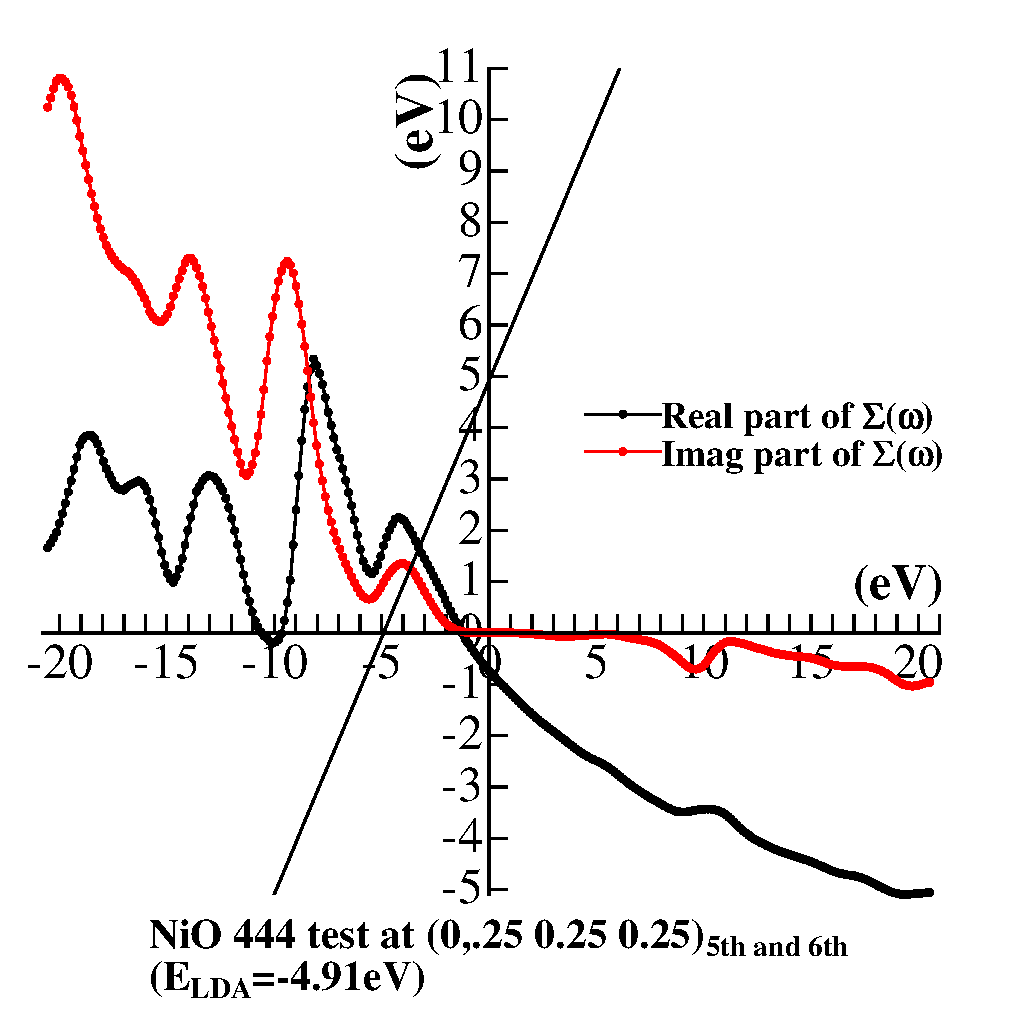
\includegraphics[width=10cm]{nio_sp1.eps}

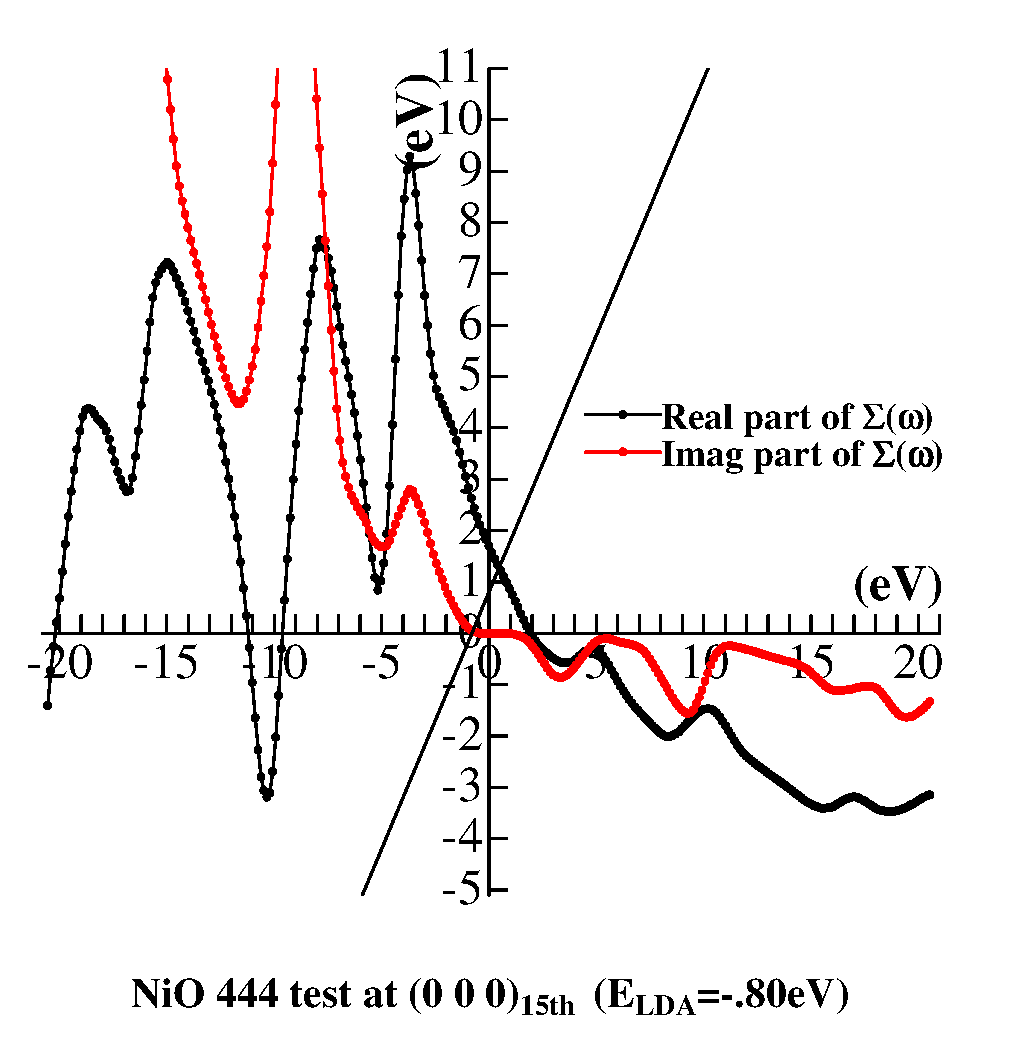
\includegraphics[width=10cm]{nio_sp2.eps}
\caption[]{A test sample of mode 4 of hsfp0 to plo $\Sigma(\omega)$. Antiferro NiO case.}
\label{niospect}
\end{figure}




%==============================================================================
\newpage
\section{extest: : To check the dependence of Ex on esmr (smering parameter)}
\baselineskip=5mm
\verb#esmr# (= $E_{\rm smear}$ in Section \ref{kint})
is the parameter which is used in {\bf hsfp0} to calculate the self-energy.
It is set in \io{GWinput}.
In {\bf hsfp0}, the poles of the Green function is assumed to have the witdth {\tt esmr}.
(Rectangular smearing or Gaussian).
As for the case of insulator, it is not essentially necessary
--- You can choose it as small enough
(too small value might causes a numerical problems --- If $E_{\rm smear}=0$,
there is a "hitting (numerical) problem" because given $\omega$ and pole of $G$ is exactly the same.
So please fix it as 0.01Ry,0.001Ry or so.)
However, in the case of metal, the size fo \raw{esmr} can affects 
the resutls. Theoretially, if you take enough number of {\bf k} points,
you can use very small {\tt esmr}.

In order to determine {\tt esmr} for given number of {\bf k} points, 
I made a test script {\bf extext}.
You can run it after you get the Coulomb matrix by {\bf hvcc}.
It means that you have to execute {\bf gw\_lmf} 
but you can stop it just after it make the Coulomb matrix:

{\baselineskip=3.5mm
\begin{verbatim}
> ~/ecal/fpgw/exec/gw_lmf cu
 OK! lmf2gw: end --- DATA4GW_V2 is written
 OK! rdata4gw
 OK! heftet mode=1 EFERMI generated
 OK! hchknw: write nw to NW          <--- ***
 OK! hbasfp0 ix=3 core mode          <--- ***
 OK! hvccfp0                         <--- ***
 OK! hsfp0: Core-exchange mode       <--- ***
 OK! hbasfp0 ix=0 normal mode
 OK! hvccfp0
\end{verbatim}}
------------------Here you can stop!
(you don't need to run some programs shown as ***  in order to execute extest.)

Then you can invoke {\bf extest} as
{\baselineskip=3.5mm
\begin{verbatim}
>extest foo
. Then you can see the console outputs as
 esmr(Ry) efermi(Ry) Sx1(eV)  Sx2 ...
    0.005 -0.028478  -16.3758  -30.3606  -30.3606  -30.3606  -31.5098  ...
    0.010 -0.027853  -16.3758  -30.3606  -30.3606  -30.3606  -31.5098  ...
    0.015 -0.027228  -16.3758  -30.3606  -30.3606  -30.3606  -31.5098  ...
\end{verbatim}}
It takes a bit long (the same as time as echo 1|hsfp0),
but other lines appeares soon successively.
The first column is {\tt esmr}, the second for the determined Fermi energy,
and $\Sigma_{\rm x}$ for eigenfunctions given in \verb#<QPNT># section.

\ 

You already saw the plots which I made by the script in Section 3.

\ 

In principle, we have to estimate the limit of the numbe of ${\bf k}$ points $\to \infty$;
then we can estimate {\tt esmr} so that it is not so small so as not to include
the strange beheviors near {\tt esmr}=0 due to the ${\bf k}$-points-number cutoff.

You see that we have smoother behevior for larger number of ${\bf k}$ points;
$14\times14\times14$ case of Cu in section 3 gives rather smooth for {\tt esmr}$>.25$ or so for $E_{\rm fermi}$.
This is a case of \keyw{GaussSmear}=off. You may need to repeat it with  {GaussSmear}=on---
In Si case, I saw that 1/3 of \raw{esmr} of \keyw{GaussSmear}=off gives similar effect.

The larger dependence for $\langle \Psi_{{\bf k} n} |\Sigma_{\rm x}| \Psi_{{\bf k} n}\rangle$ 
is for states near the $E_{\rm Fermi}$; X$_4$ X$_6$, L$_6$ in the Cu case. 
The completely flat behevior at {\tt esmr} $\to 0$ in the case of $6\times6\times6$ comes from
the fact that the intervals of states at EF are smaller than these {\tt esmr}. 
Apparently $6\times6\times6$ case miss the exchange enegy about 0.2 eV for L$_6$
though the error will be cancelled by the correlation part.
The curves for $6\times6\times6$ diverges from others at even large value {\tt esmr}=0.25 Ry in X6. 
However the difference gets small for {\tt esmr}$<0.06$. So you might be able 
to use rather small value of esmr even for $6\times6\times6$ case for Cu.
As for $10\times10\times10$ case, you can see a strange behevior in X$_6$ for {\tt esmr}$<0.025$ Ry.
So it might be better you to use larger emsr to avoid the behevior.
Apparanly it is just for exchange, and we have to do total check runs
for convergence of QPU though extest will help to give some informations
what size of {\tt esmr} will be reasonable.

It is easy and rather quick if you want to repeat extest. 
Please use {\bf extest\_repeat}.
If you want further plotting points, you edit {\bf extest\_repeat} 
(add values of {\tt esmr} in foreach loop).
In order to remove too many files and directories generated, please do \verb|rm -rf EX*|.




%%%%%%%%%%%%%%%%%%%%%%%%%%%%%%%%%%%%%%%%%%%%%%%%%%%%%%%%%%%%%%%
\section{\exe{gwsc}: QP self-consistent \GW}
\label{scgw}

With a script $gwsc$, you can do QS\GW calculation
as in \cite{scgw03}.
The procedure is as follows.
\begin{enumerate}
\item Get LDA results. \raw{rst.si}

%%%%%%%%%%%%%%%%%%%%%%%%%%%%%%%%
\item Invoke \exe{gwsc1shot}.\\
This does only a first itteration to generate \io{sigm}
containing $\Sigma -V_{\rm xc}^{\rm LDA}$.
At the end of \exe{gwsc1shot}, you will get \io{sigm}.
Before invoke it, you can set, e.g.,\\
"\verb#emax_sigm  5.00 !(Ry) emax cutoff for Sigma (Optional)#"\\
in \io{GWinput} so as to reduce the computational time.
However, this 1st itteration is to check the behevior for
$\Sigma -V_{\rm xc}^{\rm LDA}$ as fucntion of $\epsilon_{\bfk n}$.
So it meybe better to take larger \verb#emax_sigm# as possible 
(maybe larger than 5 (Ry) or above).


\item Write optional section in \io{ctrl.*}.\\
At first, you have to add HAM---RDSIG and HAM---SIGP tokens to \io{ctrl.*} 
e.g. as;
\begin{verbatim}
HAM     RDSIG=12 SIGP:3,0,0,0,2.5,0,.06,0
\end{verbatim}
%{\it ---(note {\rm SIGP:}modsgp,nmin,emin,nmax,emax,asig,bsig,efit)---}.
These are explained in lmto doc as \verb#ecal_sc/lm-6.14/doc/gw.txt#.
See the note. I give a sketch here.--------
\raw{RDSIG=12} means to add the self-energy $\Sigma -V_{\rm xc}^{\rm LDA}$
to Hamiltonian if \io{sigm.*} exists. In addition, \raw{RDSIG=12}
means that we just take approximated (extraporated) diagonal-only 
$\Sigma -V_{\rm xc}^{\rm LDA}$ for high-energy bands.
The part \verb#SIGP:modsgp,nmin,emin,nmax,emax,asig,bsig,efit# 
is how to approximate the diagonal part of high-energy bands.
\verb#emax,asig,bsig# are important quantities.
Especially \verb#emax# is the cutoff above which we only 
take extrapolated diagonal parts of $\Sigma -V_{\rm xc}^{\rm LDA}$.

After you add these tokens, invoke \exe{lmf} (See the script \io{gwsc}--- don't forget rename \io{sigm} as \io{sigm.*}).
Then you can see infomations below in standard(conosle) output 
\footnote{set larger \raw{VERBOSE} to see this info, maybe 50 or so---this info is for each $\bfk$} as;
{\small \baselineskip=2.5mm
\begin{verbatim}

 hambls: approximate sigma for states n=6 and below; and for energies E(lda)>2
state E(lda)     sig_ii     constraint  use
...
...
 33   1.402066   0.135934               0.135934
 34   1.622702   0.138711               0.138711
 35   1.649643   0.153268               0.153268
 36   1.650243   0.173259               0.173259
 37   1.650244   0.173259               0.173259
 38   1.919147   0.197660               0.197660
 39   1.919162   0.197648               0.197648
 40   1.935087   0.167100               0.167100
 41   1.935099   0.167125               0.167125
 42   1.979897   0.179666               0.179666
 43   2.110782   0.233979   0.368863    0.368863 <-- 43th 
 44   2.110789   0.233979   0.368863    0.368863 <-- 44th 
 45   2.736957   0.000000   0.418957    0.418957
 46   2.736958   0.000000   0.418957    0.418957
 47   2.737101   0.000000   0.418968    0.418968
 48   2.976955   0.000000   0.438156    0.438156
 49   3.041153   0.000000   0.443292    0.443292
...                         ^^^^^^^^---Above 43th, use extrapolated sig_ii 
...                                                (shown at "constraint" column)
...              ^^^^^^^^---Up to 44th, sig_ii are calculated
\end{verbatim}}
This shows results from a key part for the extrapolation 
to determine diagonal parts of higher bands. The third column \verb#sig_ii# is for the calculated
$\Sigma -V_{\rm xc}^{\rm LDA}$.
In this example, only $\Sigma -V_{\rm xc}^{\rm LDA}$ up to 44th state are calculated because we
used "\verb#emax_sigm  2.500 !(Ry)#" in \io{GWinput} in this case.

On the other hand, "\verb#constraint#" section is from 43th.
This means that we assign "higher bands for extrapolation" 
from 43th.
This is controlled by \raw{emax} in \raw{SIGP}.
The extrapolated values are given by \raw{asig,bsig}.
In this case, these values in "\verb#constraint#" 
correspond to \verb#asig=0 bsig=.06#.\\

At the same time you see lines as
{\small \baselineskip=2.5mm
\begin{verbatim}
 hambls: sig(low,high) = 0.0000,0.2353  fit : 0.1447 + -0.0238 * E(lda) (1768 points)
\end{verbatim}}
in the same standard output of \exe{lmf}. Here\\
\verb#fit : 0.1447 + -0.0238 * E(lda)# gives
linear fitting of \verb#sig_ii# as function of \verb#E(lda)#.
These are important informations to supply reasonable \verb#asig,bsig#.

If you want to use these values, you set asig=0.1447, bsig=-0.0238 in \verb#SIGP# token.
(however, this case is a fit up to 2.500 (Ry). So not so good. 
Negative bsig is a bit strange---it may be better to choose fitting region... See gw.txt).\\

At the end, you have to give reasonable parameters for \verb#SIGP# including \raw{asig,bsig}.
Note that you have to set \raw{emax} in \raw{SIGP} and \verb#emax_sigm# 
in \io{GWinput} so as to have some overlap, so that \verb#sig_ii# should
be determined directly or the extrapolation.
We expect that these numbers affects little to final results anyway.
With our experiences \raw{emax} in \raw{SIGP} $\sim 2.0$Ry is good for NiO and so.

Anyway see \verb#ecal_sc/lm-6.14/doc/gw.txt# for details.

\item Set \keyw{iSigMode} in \io{GWinput}. 
      and invoke \exe{gwsc}. In each itteration step, you will have\\
      *.\{{\it itt-number}\}run files. E.g, QPU.1run, QPU.2run... 
      are generated at each itteration step.
\end{enumerate}




%%%%%%%%%%%%%%%%%%%%%%%%%%%%%%%%%%%%%%%%%%%%%%%%%%%%%%%%%%%%%%%
\section{Check list for convergence}
\label{checklist}
The compuational resource is rather limited
but results could be dependent on cutoff parameters in \io{GWinput},
and on the LDA result as inputs.
So you have to schedule the convergence check carefully 
and efficiently, mainly on these points below.

\begin{itemize}
\item
LDA eigenfunctions and number of unoccupied states.

A good way to check the convergence of LDA result is
the comparison of the energy bands and the density of states
generated by FP-LMTO and some other accurate method.
Within FP-LMTO, you can check the convergence
when you enlarge the LMTO basis sets, Head and Tail; 
but the LMTO itself has difficulties to persue the convergence 
for higher unoccupied states.

Main problem could be how many unoccpied states you consider.
Our experience shows that we need to add rather large number 
of unoccupied states for good convergence even if these accuracy 
would be not so good 
\footnote{This may be related to a completeness of the basis set;
the completeness could be important from the view of `Coulomb hole' picture.}

[In \io{GWinput}, you can set the number of unoccupied states
which you take into account by
\keyw{emax\_chi0}, \keyw{emax\_sigm},\keyw{nband\_chi0}, and
\keyw{nband\_sigm}. But we now usually unset them except 
the case of scGW calculation for \keyw{emax\_sigm}.]

Actually this point is most difficult for convergence check.
You have to set up carefully some LDA results as input to check the convergence.

\vspace{2mm}

\item
Number of k points \keyw{n1n2n3}.

\item
Product basis section.
At least, \verb#lcutmx#=4 
will be necessary for atoms with d electrons.

\item
Cores.
Usually we nees to treat only the shalow cores
as {\bf core2}, others as  {\bf core1}. But you need check.
As for semi-core like $d$ bands, it is better to treat 
them by local orbital.

\item
\keyw{esmr}.
You have to be careful if metal. 
You can test it with \exe{extest}.
It might be a probelm to choose too small \verb#esmr#.

\item
\keyw{dw, omg\_c}
\keyw{niw}

It will be worth to try to check
how much the results changed due to them.
But usually \verb#dw=0.01, omg_c=0.05# is not so bad.
As for \verb#niw=6# seems to be not so bad usually, but
it is safer to check the convergence on it 
(test cases with \verb#niw=10,12,16#).

\item
\keyw{deltaw}.

$\sim 0.01$ a.u. will be not so bad. 
See two Z values shown in {\sf SXCU}. 
It is better to try to check how about the depencence on this.

\item
\keyw{CoreOrth} on. Try to test it. 
If it affects so much. The $D$ function might be too poor
due to the poor orthogonality condition 
between core and valence.


\end{itemize}

%%%%%%%%%%%%%%%%%%%%%%%%%%%%%%%%%%%%%%%%%%%%%%%%%%%%%%%%%%%%%%%
\section{EXX+RPA total energy}
There is a mode to calculate total energy, origianlly started by Dr.Miyake.
I tested it so much, but it is numerially not so satisfactory;
see Ref.I.




%==========================================================================================
\newpage
\section{Linear response calculations}
\label{linearr}
We now have these \verb#eps*# scripts in the following. 

\begin{itemize}
\item \raw{eps\_lmfh} 
   epsilon with local field correction.

\item \raw{epsPP\_lmfh}

   epsilon without local field correction.
   $1- \langle \eiqr |v|\eiqr\rangle  \langle \eiqr| \left( \chi^{0} \right) |\eiqr\rangle$


\item \raw{epsPP\_lmfh\_chipm}

    For spin susceptibility. This essentially calculate non-interacting spin susceptibility.
    Then it is used for the calculation of full spin susceptibiity with \verb#util/calj_*.F# programs
    (small quick programs). See spin wave paper.
    See spin susceptibility section Sec.\ref{xxx}.

\item \raw{eps\_lmfh\_chipm}

    This gives full non-inteacting spin susceptibility. Testing.
    We have to determine $U$ (stoner $I$) for the determination of full spin susceptibility.
    TDLDA? or so?


\item \raw{(This is old mode --- removed not) epsPP\_lmfh\_chipm\_q}

  For spin susceptibility. 
  spin susceptibility $\langle e^{iqr}| \chi(q,\omega) |e^{iqr} \rangle$
  In this script, You have to assign that isp=1 is majority, isp=2 is minority.
  This is with long wave approximation.  

\end{itemize}

---------------------

\noindent $\bullet$ \raw{*\_lmfh\_*} means histogram method. At first, we calculate its imaginary parts
  with tetrahedron technique. Then we get its real part by Hilbert transformation.\\
  You need to choose \keyw{dw,omg\_c}. 
  The width of histrgram bins are getting larger when omega gets larger.
  dw is the size of histogram-bin width at omega=0. 
  At omega=omg\_c, its width gets twiced.
  You have to choose small enough omega for spin wave mode as 0.001 Ry (Or smaller).
  omg\_c is given like 0.05 Ry or so. But sometimes it can be like 1Ry.\\

\noindent $\bullet$ \raw{epsPP} uses a a special product basis set for cases without inversion
  (actually the problem is just in how to expand exp(iqr) in the mixed basis;
   the product basis is not from phi and phidot, but from spherical bessel functions).\\

\noindent $\bullet$ \keyw{EPSrange, EPSdw} are not used for \verb#*_lmfh_*# scripts.


\begin{verbatim}
In *_lmfh_* modes( I now use little for *_lmf_* modes), you can use small enough delta.
Use small enough delta (=-1e-8 a.u.) for spin wave modes (also you can use it for 
dielectric function and GW).  This is necessary because pole is too smeared 
if you use larger delta.
\end{verbatim}



%%%%%%%%%%%%%%%%%%%%%%%%%%%%%%%%%%%%%%%%%%%%%%%%%%%%%%%%%%%%%%%%
\section{eps\_lmfh, epsPP\_lmfh: the dielectric functions}

You can invoke the script, e.g. as "\exe{eps\_lmfh} \ si".

----------------

Specify ${\bf q}$ point in \verb#<QforEPS># or so.
Mesh for $\omega$ is specified by \keyw{dw, omg\_c}.

The obtained datas are in {\sf EPS*.dat} and {\sf EPS*.nlfc.dat}.
{\sf EPS*.nlfc.dat} contains the result without local-field correction
{\sf EPS*.dat} contains the result with local-field correction
(this is generated only for \verb#eps_lmfh#. Both of them contains

{\bf q}(1:3), $\omega$, Re($\epsilon$) Im($\epsilon$), Re(1/$\epsilon$), In(1/$\epsilon$)\\
in each line.

For the limit ${\bf q} \to 0$, be careful!
Because ${\bf q} \to 0$ gives too large cancelation effects
(the denominator and numerator go to zero---it means we need very accurate
orthogonalization between occupied and unoccupied states).
This is a kind of disadvantage of our method (though there is an advantage---
our code can calculate dielectric function even for metal 
as far as you use large enough number of ${\bf k}$ point.)

The calculaten of dielectric functions usually requires so many $k$ point. 
For example, for si,  \verb#n1 n2 n3 = 4 4 4# is too small. 
It gives too large dielectric constants $\sim19.4$ though
the converged value should be $\sim13$. (we need 10x10x10 or more like 20x20x20
for some reasonable results).
For GaAs, we observed that reasonable $\epsilon(\omega)$ requires
rather large number of ${\bf q}$ points lke 15x15x15 or 20x20x20
for \keyw{n1n2n3}. This is too time-consuming to get result
(but you can use ``very small product basis''(just sp poralization for this purpose;
it makes speed up so much). Or, you can calculate "$\epsilon(\omega)$ without LFC". 
See section for \exe{eps\_PP\_lmfh}.

----------\underline{\bf !WARNING!}-------------\\
\noindent 1. This code works OK only for ${\bf q}$ is near 0.
Be careful for ${\bf q} \to 0$ limit. Too small ${\bf q}$ can give strange
spectrum at high energy (real part is affected by it)\\

\noindent 2. \keyw{CoreOrth} gives so serious effect for 
$\epsilon(\omega)$, if you include some cores as "{\bf core2}"
in the product basis setting.
(This means that you includes transtions from "{\bf core2} to
valence" in the calculation of $\epsilon(\omega)$).

Then you have to use "\raw{CoreOrth} on". Without it,
you will have rather large imaginary part at rather high energy
Such transitions from core to higher valence bands
is artifical due to the incomplete orthogonality
between core and the higher bands.
However, shallower $d$ semi-core might be deformed too much
by this option. Try to plot \io{Core\_*.chk} files, 
which contains core radial functions. 
Anyway, it is better to treat shallow core as valence by ``local orbital''.


%%%%%%%%%%%%%%%%%
\subsection{epsPP\_lmfh: the dielectric function(No LFC--- faster)}

You can calculate $\epsilon$ without LFC by
{\bf epsPP\_lmfh}. It is very faster than \exe{eps\_lmfh}.

To calculate $\epsilon({\bf q},\omega)$ without LFC accurately,
the best basis set for the expantion of the Coulomb matrix within MT
is apparently not the product basis, but the bessel functions
corresponding to the plane waves $\exp(i{\bf q r})$.
We use such a basis in this mode. 
However, our experience shows that the changes are little even 
with the usual product basis (we don't describe this here).
%You can test it by the script {\bf epsPtestNoLfc\_nfp}. 
%Please check the script whether it sets the {\bf q}
%point which you want to calculate.
%{\bf epsPtestNoLfc\_nfp} runs \verb#echo 3|hsfp0#. 
%The mode 3 only gives files {\sf  EPSxx.nolfc.dat}.
%
%Apparently you don't needs to do {\bf eps\_lmf} if you just change the file
%{\sf EPS\_cond}; then you just need to run \verb#echo 4|hsfp0#.



%%%%%%%%%%%%%%%%%%%%%%%%%%%%%%%%%%%%%%%%%%%%%%%%%%
\section{How to calculate correct epsilon?}

\begin{verbatim}

There are prolems to calculate correct epsilon.
At first, we talk about epsPP_lmfh, which is No LFC. Main problem are 

-----------------
1.Convergence for number of k point(specified by n1n2n3). 
  Roughly speaking, 20x20x20 is required for not-so-bad results for Fe and Ni.
  It is better to do 30x30x30 to see convergence check.
  However, in the case of ZB-MnAs (maybe because of simple structure around Ef),
  it requires less q points.

  figs are for GaAs.
  fig001: n1n2n3 convergence for Chi_RegQbz = on  case.
  fig002: n1n2n3 convergence for Chi_RegQbz = off case.
  (Chi_RegQbz in explained in General section in this manual).

  As you see, k points convergence looks a little better in Chi_RegQbz=off
  (mesh not including gamma). However a little ploblem is that its thereshold around 
  0.5eV is too high and slowly changing.

  fig003: Alouanis'(from Arnaud)  vs. ``Chi_RegQbz = on'' vs. ``Chi_RegQbz = off''
  As you see, the threshold of the Red line (20x20x20 Chi_RegQbz=on) and Alouani's 
  are almost the same, but the red line is too oscilating at the low energy part.
  On the other hand, ``Chi_RegQbz = off'' in Green broken line is not so satisfactory
  at the low energy part. 

  fig.gas_eps_kconf.pdf shows the convergence behevior of epsilon for 
  
   
2.$q \to 0$ convergence (this is related to whether Chi_RegQbz=on or off).
  If you use very small q like q=0.001 is GaAs, it can cause a problem.
  Use q=0.01 or larger (maybe q=0.02 or more is safer). 
  Very small q can give numerical error for high-energy region.

  In fig004, we show the high energy tail part of Im $\epsilon(\omega)$ for GaAs case.
  At q=0.01 (this means q= 2*pi/alat * (0 0 0.01)), the imaginary part
  is a little too large . Less than 80eV, q=0.02 gives good results when compared with
  other high q results, though it still has noise above 80eV.
  In fig005, I showed the same results compared with Alouani's (his is up to 40eV).
  Both gives rather good agreements. As you see, q=0.06 or above might be necessary
  to get reasonable convergence for high energy part abouve 40eV.

  We have to be careful for this poorness in high energy part--- it may effect
  low-energy Re[$\epsion$] through KK relation. However this can be very small
  ehough.
  In fig.gas_eps_qconv.jpg, we checked the convergence of eps (\omega=0,q) for q \to 0.
  As you see, it gives convergence, however, q=0.01 is a little out of 
  curve---this should be because of the poorness in the high energy part.
  so q=0.02 or q=0.03 is safer, and you can get eps within 1 percenr accuracy.

3. Including Core for dielectric constant is dangerous. 
   It can cause very poor results if you include core part in GWinput.
   You need to include core just as valence (with local orbital).

   In fig008, we showed core effects. It starts from \approx 16eV 
   (this is core to conduction transition).
   fig007 showd the check about the q point dependence---even with large q,
   it would not change.
   These shows that the core excitation can have larger energy range.
   This is in contrast to the valence case 
   (then the most of excitaion is limited to less than 10eV).
   We have to be careful for such high-energy exciation... The LMTO basis might
   be not so good for high energy.

4. basis set.
   Use QpGcut_psi \approx 3.0 a.u. or so (as same as GW calculation).
   In the case of epsPP* mode, 
   QpGcut_cou can be very small--- In our codes now, 
   ngc>=1 should be for all q vector shown in lqg4gw02 (output of echo 2|qg4gw).
   [In principle, it should be only for the q vector for which we calculate epsilon.
    But there is a technical poorness in our code---
    (maybe) a problem here; the plane-wave part of the eigenfunction generated 
    in lmfgw is not correctly passed to lmf2gw when ngc=0].


-- eps_lmfh: including LFC ----------------------------------
To include eps with LFC, do eps_lmfh. 
But lcutmx=2 seems to be good enough to get 0.5 percent error (maybe better than this).
Test it 10x10x10 or so. (I need to repeat if necessary).
Further you can use smaller QpGcut_cou like 2.2 or so, 
with rather smaller product basis (up to p timed d, not including f).

Note: epsPP_lmfh is designed to use good basis to calculate eps 
without LFC. This is usually in agreement with what you obtained by eps_lmfh;
however it can give slight difference when you use small product basis.


---Summary --------------------
So in conclusion, I think a best way to do is

1. set q=0.02 [q=2pi/alat(0 0 0.02)] or so for GaAs case.
   If you want to check, do q=0.03 and q=0.06 also.

   ``Chi_RegQbz = off'' is better for matrials like GaAs with direct gap.

2. You can use small QpGcut_cou but all ngc should be one or more.

3. As for the Product basis setting in epsPP* scripts, only
   lcutmx and tolerance (this can be like 0.001 or so) are relevant.
   E.g. set lcutmx=4 or so.

4. Do nk=20 18 16 and take interpolarion to determine eps(omega=0, q=0).

5. To get eps with LFC, set QpGcut_cut as xxx, and set lcutmx=2 where
   (occupied sp) \timex (unoccupied spd) are included.
   But correct EPS*.nolfc.d is rather from epsPP_lmfh script.

\end{verbatim}


\figp{gas_fig001.eps}

fig001

\figp{gas_fig002.eps}

fig002

%\begin{center}
\figp{gas_fig003.eps}

fig003


\figp{gas_fig004.eps}\\
fig004

\figp{gas_fig005.eps}\\
fig005

\figp{gas_fig007.eps}\\
fig007

\figp{gas_fig008.eps}\\
fig008
 


%%%%%%%%%%%%%%%%%%%%%%%%%%%%%%%%%%%%%%%%%%%%%%%%%%%%%%%%%%%%%%%%%%%%%%%%%%%%%%%%%%%%%%
\newpage

\section{$\chi^{+-}$ calculation} 
\label{chipmcal}
[I changed sign of $\chi$! (July2007); This definition may be different from other text book. Be careful]
The non-interacting transverse spin susceptibility 
$\chi^{0+-}(\bfr,\bfr',t-t')$ is given as
\begin{eqnarray}
\chi^{0+-}(\bfr,\bfr',t-t') = 
-i\langle T(S_+(\bfr,t) S_-(\bfr',t') \rangle
=- i G_\isptwo(\bfr,\bfr',t-t') G_\ispone(\bfr',\bfr,t'-t) 
\label{generalchi0t}
\end{eqnarray}
for non-interacting system (Lindhard-like poralization function).
In $\omega$ space, this reduced to
\begin{eqnarray}
&&\chi^{0+-}(\bfr,\bfr',\omega) \nonumber \\
%= 
%  G_\isptwo(\bfr,\bfr',\omega) \otimes G_\ispone(\bfr,\bfr',-\omega) 
%=
%    G^{\rm e}_\isptwo(\omega) \otimes G^{\rm h}_\ispone(-\omega) 
%  + G^{\rm h}_\isptwo(\omega) \otimes G^{\rm e}_\ispone(-\omega)   \nonumber \\
&&= 
\sum^{\rm  occ}_{n \ispone} \sum^{\rm  unocc}_{n'\isptwo}
\frac{
\Psi_{n\ispone}^*(\bfr)      \Psi_{n'\isptwo}(\bfr)
\Psi_{n'\isptwo}^*(\bfr') \Psi_{n\ispone}(\bfr') 
}{\omega-(\epsilon_{n'\isptwo}-\epsilon_{n\ispone})+i \delta} 
+ \sum^{\rm  unocc}_{n \ispone} \sum^{\rm occ}_{n'\isptwo}
\frac{
\Psi_{n\ispone}^*(\bfr)      \Psi_{n'\isptwo}(\bfr)
\Psi_{n'\isptwo}^*(\bfr') \Psi_{n\ispone}(\bfr') 
}{-\omega-(\epsilon_{n\ispone}-\epsilon_{n'\isptwo})+i \delta},
\label{generalchi0}
\end{eqnarray}
%where $\otimes$ means convolution as for $\omega$;  $f(\omega) \otimes g(\omega)
%= \int_{-\infty}^{\infty} \frac{i d \omega}{2\pi} f(\omega-\omega') g(\omega')$.
Here $\ispone$ is for majority ({\tt isp=1}) and 
$\isptwo$ is for minority ({\tt isp=2}), 
$\left(
 \begin{array}{c} {\rm isp=1} \\ 
                  {\rm isp=2} 
  \end{array}   
\right) =
\left(
 \begin{array}{c} \ispone \\ 
                 \isptwo 
  \end{array}   
\right)$. \\
   
\noindent $S^+(\bfr) = \Psi_{\rm isp=1}^*(\bfr) \Psi_{\rm isp=2}(\bfr) 
= \Psi_{\rm \ispone}^*(\bfr) \Psi_{\rm \isptwo}(\bfr)$, 

\noindent $S^-(\bfr') = \Psi_{\rm isp=2}^*(\bfr') \Psi_{\rm isp=1}(\bfr') 
= \Psi_{\rm \isptwo}^*(\bfr') \Psi_{\rm \ispone}(\bfr')$, \ 



\noindent Notes:
\begin{itemize}
\item This definition of $\chi^{0+-}$ 
results in $\chi^{0+-} \to \frac{\rm m}{\omega-\Delta_{\rm ex}}$
at ${\bf q}=0$ in the case of shifted-band model as 
$\epsilon_\bfk^\isptwo = \epsilon_\bfk^\ispone + \Delta_{\rm ex}$.
Here $\Delta_{\rm ex}$ means exchange splitting, and $m = N_\ispone- N_\isptwo$.
For paramagnetic case, this definition gives $\chi_0 = 2 \chi^{0+-}$, where
 $\chi_0$ is usual Lindhard polarization function for density response.
%(Because of this, our program rather show $-\chi^{0+-}$ in {\tt \bf ChiPM*} file.

\item Recall 
$ e^{-i (\eps-\eps') t} \theta(t)  = e^{-i \eps t} \theta(t) \times e^{+i \eps' t} \theta(t)$ 
or equivalently 
$ \frac{1}{\omega-(\eps-\eps')+i \delta}= \int d\omega' \frac{1}{\omega-\omega'-\eps+i \delta} \frac{1}{-\omega'-\eps'-i \delta}$.

\item If no occupation for minority channel, only the 1st term in \req{generalchi0} remains.
In contract to charge density, $\chi^{0+-}$ is not symmetric for $\omega \leftrightarrow -\omega$. 
\end{itemize}

By the way, the physically meaningful quantity is the retarted verion of $\chi^{0+-}$,
named as $\chi^{0+-}_{\rm Ret}$, which is given by changing the sign of $+ i \delta$ in \req{generalchi0}
so as to make it propotional to $\theta(t)$.
Let us assume colinear case (z-axis), 
and consider adding external transversal magnetic fiels $B_x(\bfr,t)$ and $B_y(\bfr,t)$ 
for our system. For non-interacting system, this $\chi^{0+-}_{\rm Ret}$ 
specify the linear repsonse to such $B_x$ and $B_y$.
Instead of them, it is convenient to use the complex field, $b^- = b_x -i b_y$,
(I introduce ${\bf b}$ in unit of 
$g \mu_{\rm B}/2$, so that $(g \mu_{\rm B}/2) B_x =  b_x$:
electron's spin magnetic momenets is $-2 g \mu_{\rm B} {\bf s}$.)
Then the additional Hamiltonian due to this magnetic field is written
as 
\begin{eqnarray}
H_{\rm ext\_mag} 
&=&  \int d^3r B(\bfr) \cdot g \mu_{\rm B} {\bf s}(\bfr)
=  2 \int d^3r {\bf b}(\bfr) \cdot {\bf s} (\bfr) \nonumber \\
&=&  \int d^3r \left[ b^+(\bfr) s^-(\bfr) + b^-(\bfr)s^+(\bfr) 
+ 2 b_z(\bfr) s_z(\bfr) \right],
\end{eqnarray}
where $s^-(\bfr) = s_x(\bfr)- i s_y(\bfr)$ and so on.
$\ds s_x(\bfr) = \sum_{\alpha,\beta} 
\langle \hat{\psi}^\dagger_\alpha(\bfr) \frac{1}{2} \sigma^x_{\alpha \beta}
\hat{\psi}_{\beta}(\bfr) \rangle $
and so on, where $\sigma^x_{\alpha \beta}$ is the Pauli matrix.
The induced spin moment $\D s^-$ for non-interacting system is given as
\begin{eqnarray}
&& \D s^-(\bfr,t) = \int dt' d^3r' \! \chi^{0+-}_{\rm Ret}(\bfr,\bfr',t-t') b^-(\bfr',t').
\end{eqnarray}
[because of $\theta(t)$ in  $\chi^{0+-}_{\rm Ret}$, $t-t'>0$.].

In the case of interacting system, we need to construct $\chi^{+-}$.
We define ${U}(\bfr,\bfr',\omega)$ as
\begin{eqnarray}
(\chi^{+-})^{-1} =  \left(\chi^{0+-}\right)^{-1} - {U}.
\label{chirpa0}
\end{eqnarray}
This is taken as the definition of ${U}(\bfr,\bfr',\omega)$.
How to define $U$ is the problem --- See my {\bf spin wave paper} in Arxiv.
We utilize one degree of freedome per atom (so $\chi^{+-}$ is 
the matrix whose dimension is the number of magnetic atoms), and sum rule.
(Some one may call this approximation as ``rigid moment approximation''.
 But it can be misleagind. Be careful about what I did.


\noindent ----MEMO----------------------\\
{\bf \tt eps\_lmfh\_chipm}: Our fpgw code can calculate
$\chi^{0+-}$ in this form of expansion
\begin{eqnarray}
\chi^{0+-}(\bfr,\bfr',\omega) 
= \frac{1}{N}\sum_q \chi^{+-}_\bfq(\bfr,\bfr',\omega)
= \frac{1}{N}\sum_q \sum_I \sum_J
M^\bfq_I(\bfr) \chi^{0+-}_{\bfq IJ}(\omega) (M^\bfq_J(\bfr'))^*.
\label{chiexpand}
\end{eqnarray}
Here $\{ M^\bfq_I(\bfr) \}$ is the complete set with the periodicity specified 
by $\bfq$ (Mixed basis).
In other words, $\{ M^\bfq_I(\bfr) /e^{i \bfq \bfr} \}$ 
is the complete set to expand periodic function.
However, I have not used this now...;problem is determination of $U$. How to do it?
(sum rule is not enough. we need static response?).


\section{Sum rule(moment)} 
The equation of motion of spin is written as
\begin{eqnarray}
i \dot{\hat{\bf S}} = [\hat{\bf S},  \hat{H}]
\end{eqnarray}
\begin{eqnarray}
\chi^{+-}(\bfr,\bfr',t-t') 
&=& -i\langle T\left( S_+(\bfr,t) S_-(\bfr',t') \right) \rangle                \nonumber\\
&=& -i\langle S_+(\bfr,t)   S_-(\bfr',t') \rangle \theta(t-t')
+ i\langle S_-(\bfr',t') S_+(\bfr,t)   \rangle \theta(t'-t)
\end{eqnarray}
Thus
\begin{eqnarray}
&&\frac{\partial }{\partial t} \chi^{+-}(\bfr,\bfr',t-t') 
= -i [S_+(\bfr,t),   S_-(\bfr',t)] \delta(t-t') \nonumber\\
&&-  \langle [S_+(\bfr,t),H]   S_-(\bfr',t') \rangle \theta(t-t') 
+  \langle S_-(\bfr',t')   [S_+(\bfr,t),H] \rangle \theta(t'-t),
\end{eqnarray}
where $[S_+(\bfr,t), S_-(\bfr',t)]= 2S_z(\bfr,t) \delta(\bfr-\bfr')$.
As $\int d^3r [S_+(\bfr,t),H]=0$, we have
\begin{eqnarray}
&&\int d^3r \frac{\partial }{\partial t} \chi^{+-}(\bfr,\bfr',t-t') 
= -i \langle [S_+(\bfr,t),   S_-(\bfr',t)] \rangle \delta(t-t') 
= -2 i \langle S_z(\bfr,t) \rangle \delta(t-t') 
\end{eqnarray}
This reads
\begin{eqnarray}
&&\int d^3r \omega \chi^{+-}(\bfr,\bfr',\omega) 
= 2 \langle S_z(\bfr',t) \rangle = M_z(\bfr') 
\end{eqnarray}

\noindent $\bullet$ At $\omega \to \infty$, this condition get stronger as
\begin{eqnarray}
\chi^{+-}(\bfr',\bfr,\omega) \to
\frac{M(\bfr)}{\omega} \delta(\bfr-\bfr') + O(1/\omega^2).
\label{summ2}
\end{eqnarray}
See {\bf spin wave paper}.


\section{Rigid moment approximation} 
This means that ``the magnetic moments are very rigid that they
changes without changing its form''. 
In other words, $\D s^-(\bfr)$ induced by any $b_-(\bfr)$ 
are propotional to its original moment $s_z(\bfr)$.
Rigid rotation in spin space can be expressed by e.g.,
$\ds U^x(\theta)=\exp\left( \frac{i \sigma^x \theta}{2}\right)$ in the case of x-axis rotation.
Then you can easily verify
$(U^x(\theta))^\dagger \sigma^z U^x(\theta) \propto \sigma^y$
This means $\D s^-(\bfr) \propto s_z(\bfr)$. 
Note that we did rotation only in spin space.
We neglect the mappling of $\bfr$ when we rotate spin---this will cause
little problem when the moment is rather spherical.
Be careful; our approximation (one-degree of freedom per magnetic atom) 
may be a little different from the ``rigid moment approximation''.
I did not want to mix it up, thus I avoided this terminology in my {\bf [spin wave paper]}.



%% %%%%%%%%%%%%%%%%%%%%%%%%%%%%%%%%%%%%%
%% \newpage
%% \begin{figure}[ht]
%% %\begin{center}
%% \vspace{-3cm}

%% \figs{SpinNi_000013_line100.eps}{SpinNi_000017_line100.eps}

%% \figs{SpinNi_000020_line100.eps}{SpinNi_000022_line100.eps}

%% %\end{center}
%% \caption[]{ Ni-100(a=6.640(experimental) or 6.481(da159---LDA value) a.u.)$\times$(LDA or \scgw) :  
%% {$\ds {\rm Im} \left[ \frac{\langle m| \chi^{+-} |m \rangle}{\langle m|m \rangle^2} \right]$.}
%% We used Eq.(\ref{chieq}),Eq.(\ref{chiinv}) and Eq.(\ref{chipmnolfc}) (Without LFC).}
%% \label{Nichipmnolfc100}
%% \end{figure}

%% \newpage
%% \begin{figure}[ht]
%% %\begin{center}
%% \vspace{-3cm}

%% \figs{SpinNi_000015_line111.eps}{SpinNi_000018_line111.eps}

%% \figs{SpinNi_000021_line111.eps}{SpinNi_000023_line111.eps}

%% %\end{center}
%% \caption[]{ Ni-111. Same as Fig.\ref{Nichipmnolfc100}.}
%% \label{Nichipmnolfc111}
%% \end{figure}


%% %%%%%%%%%%%%%%%%%%%%%%%%%%%%%%%%%%%%%%%%%%%%%%%%%%%%%%%%%%%%%%%%%%%%%%%
%% \newpage
%% \begin{figure}[ht]
%% %\begin{center}
%% \vspace{-3cm}

%% \figs{SpinFe_000025_line100.eps}{SpinFe_000027_line100.eps}

%% \figs{SpinFesc_line100.eps}{SpinFesc_da197_line100.eps}

%% %\end{center}
%% \caption[]{ Fe-100(a=5.408(experimental) or 5.211(da197---LDA value) a.u.)$\times$(LDA or \scgw) :  
%% {$\ds {\rm Im} \left[ \frac{\langle m| \chi^{+-} |m \rangle}{\langle m|m \rangle^2} \right]$.}
%% We used Eq.(\ref{chieq}),Eq.(\ref{chiinv}) and Eq.(\ref{chipmnolfc}) (Without LFC).}
%% \label{Fechipmnolfc100}
%% \end{figure}


%% %%%%%%%%%%%%%%%%%%%%%%%%%%%%%%%%%%%%%%%%%%%%%%%%%%%%%%%%%%%%%%%%%%%%%%%
%% \newpage
%% \begin{figure}[ht]
%% %\begin{center}
%% \vspace{-3cm}

%% \figs{SpinFe_000026_line110.eps}{SpinFe_000028_line110.eps}

%% \figs{SpinFesc_line110.eps}{SpinFesc_da197_line110.eps}
%% %SpinFe_000032_line110.eps}

%% %\end{center}
%% \caption[]{ Fe-110. Same as Fig.\ref{Fechipmnolfc100}.}
%% \label{Fechipmnolfc110}
%% \end{figure}



%%%%%%%%%%%%%%%%%%%%%%%%%%%%%%%%%%%%%%%%%%%%%%%%%%%%%%%%%%%%%%%%%5
\newpage
\section{static $J(q)$ calculation---- Heisenberg Model}
(See kotani's SW paper).
The total energy of our spin system is assumed to be
\begin{eqnarray}
&& {\cal H} = - \sum_{Rn} \sum_{R'n'} 
J_{Rn R'n'} \bfS_{Rn} \cdot \bfS_{R'n'} + g \mu_B \sum_{Rn} 
\bfS_{Rn} \cdot \bfB_{Rn}
\label{hei1}
\end{eqnarray}
. Here we take all site indexes $Rn$ and $R'n'$ 
($J_{RnRn}=0$. $J_{RnR'n'}=J_{R'n'Rn}$. 
It we restrict sum as $Rn>R'n'$, factor 2 appears.).
$\bfS_{Rn}$ is the spin at $Rn$ ($R$ is for primitive cell, $n$ specify
site in a cell).
The equation of motion 
$-i\hbar \dot{\bfS}_{Rn} = [{\cal H} , {\bfS}_{Rn}]$,
is reduced to be
\begin{eqnarray}
\hbar \dot{\bfS}_{Rn} = \bfS_{Rn} \times 
\left(2 \sum_{R'n'} J_{Rn R'n'} \bfS_{R'n'} - g \mu_B \bfB_{Rn} \right)
\label{hei2}
\end{eqnarray}
We introduce $g \mu_B \bfB = 2 \bfb$, and $\bfS_{Rn}=\bfS_{Rn}^0 + 
\bfiS_{Rn}$. Then \req{hei2} reduce to
\begin{eqnarray}
&&\hbar \dot{\bfiS}_{Rn} =  \bfS^0_{Rn} \times
\left(2 \sum_{R'n'} J_{Rn R'n'} \bfiS_{R'n'}  \right)
+ \bfiS_{Rn} \times 
\left(2 \sum_{R'n'} J_{Rn R'n'} \bfS_{R'n'} \right)
- 2 \bfS^0_{Rn} \times \bfb_{Rn} \nonumber \\
&&= \sum_{R'n'} \left(2 \bfS^0_{Rn} J_{Rn R'n'} \right) \times \bfiS_{R'n'}
- 
\left(2 \sum_{R'n'} J_{Rn R'n'} \bfS^0_{R'n'} \right)  \times \bfiS_{Rn} 
- 2 \bfS^0_{Rn} \times \bfb_{Rn} 
\label{hei3}
\end{eqnarray}
Introduce the fourier transformation as
$\bfiS_{Rn} = \frac{1}{N} \sum_\bfk \bfiS_n(\bfk) e^{i \bfk \bfR}$.
Then \req{heis3} reduce to
\begin{eqnarray}
&&\hbar \dot{\bfiS}_{n}(\bfk)   
= \sum_{n'} \left( 2 \bfS^0_{n} J_{n n'}(\bfk) 
- \left(2 \sum_{n''} J_{n n''}(0) \bfS_{n''}^0\right) \delta_{nn'}\right)  \times \bfiS_{n'}(\bfk)
- 2 \bfS^0_{n} \times \bfb_{n}(\bfk).
\label{hei4}
\end{eqnarray}
Assume $\ds {\bfiS}_{n}(\bfk) \propto e^{-i \frac{\omega t}{\hbar}}$,
we have 
\begin{eqnarray}
 \sum_{n'} \left(\frac{i \omega \delta_{nn'}}{2} +  \bfS^0_{n} J_{n n'}(\bfk) 
- \left( \sum_{n''} J_{n n''}(0) \bfS_{n''}^0\right) \delta_{nn'}\right)  \times \bfiS_{n'}(\bfk)
= \bfS^0_{n} \times \bfb_{n}(\bfk).
\label{hei5}
\end{eqnarray}
Let us consider colinear ground state, then $\bfS^0_{n}= S_n \bfe_z$
($S_n$ is the size of spin with sign). You have
\begin{eqnarray}
\sum_{n'} \left( \frac{i \omega \delta_{nn'}}{2S_n} \right) \bfiS_{n'}(\bfk)
+\sum_{n'} \left( J_{n n'}(\bfk) 
- \left( \sum_{n''} \frac{1}{S_n} J_{n n''}(0) S_{n''} \right) \delta_{nn'}\right)  \bfez \times \bfiS_{n'}(\bfk)
=  \bfez \times \bfb_{n}(\bfk).
\label{hei6}
\end{eqnarray}
As $\bfS = S^+ \frac{\bfex -i \bfey}{2}
         + S^- \frac{\bfex +i \bfey}{2} + S^z \bfez$,
and $\bfez \times ({\bfex \pm i \bfey}) = \mp i({\bfex \pm i \bfey})$
we have,
\begin{eqnarray}
&&\sum_{n'} \left( \frac{\omega \delta_{nn'}} {2S_n} -
 \bar{J}_{n n'}(\bfk) \right)  S^+_{n'}(\bfk)
=  b^+_{n}(\bfk). \\
&&\sum_{n'} \left( \frac{\omega \delta_{nn'}} {2S_n} + 
\bar{J}_{nn'}(\bfk)  \right)    S^-_{n'}(\bfk)
=  b^-_{n}(\bfk),
\end{eqnarray}
where
\begin{eqnarray}
\bar{J}_{nn'}(\bfk)=  J_{n n'}(\bfk) 
- \left( \sum_{n''} \frac{1}{S_n} J_{n n''}(0) S_{n''} \right) \delta_{nn'}
\label{jbar}
\end{eqnarray}
This $\bar{J}_{nn'}(\bfk)$ and also $S_n $ are stored in \verb#Jmat# file
(or \verb#JMAT# line when you run a script \verb#ecal/util/calj\_summary_mat# 
which calls (\verb#calj_nlfc_mat#). 
Only the differenc between $\bar{J}_{nn'}(\bfk)$ and $J_{n n'}(\bfk)$
are diagonal parts. 
These are determined so that $\int d^3k {J}_{nn}(\bfk)=0$.\\

\noindent JJMAT contains another definition of $J$, which is to reproduce SW spectrum
(but it does not work well in cases because the SW peaks are not well identified at high $\bfk$.)\\

See my spin wave paper.


\section{$J(q)$ and Tc}
---- this section is my memo. Not need to read here ----

(This section is not consistent with previous page. Only a case, with an atom in the cell).
The total energy of our spin system is assumed to be
\begin{eqnarray}
&& E_{\rm spin} = - \sum_i \sum_j J_{ij} \bfe_i \cdot \bfe_j
\label{heis1}
\end{eqnarray}
. Here we take all site indexes $i$ and $j$ 
($J_{ii}=0$. $J_{ij}=J_{ji}$. 
It we restrict sum as $i>j$, factor 2 appears.).
$\bfe_i$ is the unit vector to specify the spin direction.

%% $\chi^{+-}(\bfq) \equiv \chi^{+-}(\bfq, \omega=0)$
%% gives the static energy difference for the spin system 
%% within the linear response scheme. 
%% Consider the linear response based on \req{heis1}, 
%% $J(\bfq)$ should satisfy
%% \begin{eqnarray}
%% J(\bfq) - J(0) = -\langle m| \left( \chi^{+-}(\bfq) \right)^{-1} |m \rangle 
%% =
%% - \langle m| \left( \chi^{0+-}(\bfq) \right)^{-1} |m \rangle 
%% + \langle m| I |m \rangle.
%% \label{jdiff}
%% \end{eqnarray}
%% Here we used Eq.(\ref{chieq}) and 
%% $\langle m| I |m \rangle= \langle m|
%% \left( \chi^{0+-}(\bfq=0,\omega=0) \right)^{-1}|m \rangle$
%% as in Eq.(\ref{sp0cond}).

If we identify $ E_{\rm spin}$ as the Heisenberg hamiltonian
with a fixed spin moment $m = N^{\ispone}- N^{\isptwo}$,
the spin wave dispersion is given as
\begin{eqnarray}
\omega_\bfq = \frac{4}{m} \left[ J(0) -J(\bfq) \right].
\label{omegaq}
\end{eqnarray}
This $\omega_\bfq$ is different from the true pole of 
$\langle m| \left( \chi^{+-}(\bfq,\omega) \right)^{-1} |m \rangle$ 
 except
$\bfq \to 0$.

The critical temperature $T_{\rm c}$ is given as
$T_{\rm c} = \frac{2}{3} J(\bfQ) Q_{\rm factor}$.
This $Q_{\rm factor}$ can be $(S+1)/S$, but 
it seems to be taken as unity usually...
$J(Q=0)$ is for ferromagnetic case.

In order to calculate $J(0)$,
integrate the left hand side of Eq.(\ref{jdiff}) in the BZ
and use $\ds \int \frac{\Omega d^3 q}{2 \pi} J(\bfq)=0$. It gives

\begin{eqnarray}
T_{\rm c} = \frac{2}{3} J(0) = 
\frac{2}{3} \int \frac{\Omega d^3 q}{2 \pi}
\langle m| \left( \chi^{+-}(\bfq) \right)^{-1} |m \rangle 
= 
\frac{2}{3} \frac{m}{4} \int \frac{\Omega d^3 q}{2 \pi} \omega_\bfq 
\label{tceq}
\end{eqnarray}

This equation contains two probrems.
\begin{enumerate}
\item[(1)] Mapping to a Heisenberg model.\\
This may cause a problem in the case of transition metals, and so.
The spin waves have strong dumping.
Further, we don't include the temperature-dependence of the model itself.

%$\omega_\bfq$ around BZ boundaries can be
%very different from \req{omegaq}.
%However, this mapping may be not so problematic for insulators---
%no Stonar dumping case (exactly speaking, no dumping channel to quasi particle pairs).\\
%For Ni, ${omegaq} \approx$ 800 meV at q=(100), 
%though the spin-wave spectrum has rather sharp peak around 550meV 
%(the peak is originally from the structure of $Im(\chi_0(\omega))$).
%For Fe, it shows 


\item[(2)] Mean field apprximation to solve the Heisenberg model.\\ 
In other words, $Q_{\rm factor}$ should be a functional of $J(\bfq)$ for all $\bfq$.
We can devide the problem into classical part and quantum part.
A contraversial point is that the integral in \req{tceq} 
is rather dominanted by the contribution around the BZ boundaries,
though we can expect that $T_{\rm c}$ can be rather strongly controlled
by low energy $\omega_\bfq$. 

\end{enumerate}

~\\

--- (this is Mark says)---

[MF Quantum Tc] --- too high.  (S+1)/S * MFC

[Full Quantum Tc] --- Exact solution of the Heisenberg Model.

[MF Classical Tc] 

[Full Classical Tc] (probably $\sim$ 80 \% of MFC)



%%%%%%%%%%%%%%%%%%%%%%%%%%%%%%%%%%%%%%%%%%%%%%%%%%%%%%%%%%%%%%%%%%%%%%%
\newpage
\begin{figure}[hbpt]
\begin{center}
\vspace{-3cm}
\includegraphics[width=12cm]{ZBmnasw1.eps}
\end{center}
\caption[]{
[{\Large We have to recalculate this!!!}]
$\omega_\bfq$ for ZincBlend MnAs by Eq.\ref{omegaq}. 
LDA case vs. \scgw case. 
\scgw makes ZincBlend MnAs as half-metallic. 
m denotes on-site moment in $\mu_B$. 
The mean-filed $T_c$ in \scgw is about 600 K.}
\label{zbmnas}
\end{figure}




%%%%%%%%%%%%%%%%%%%%%%%%%%%%%%%%%%%
\newpage
{\huge --- Notes in {\bf fpgw032f06f.tar.gz} -----}
\section{eqs. for Fourer transformation in {\bf fpgw} program}

(I think this section is still meaanigful for my code).\\

Any site-dependent functions $A(\bfR)$ are written as
\begin{eqnarray}
&& \bar{A}(\bfk) = \sum_{R} A(\bfR) e^{-i \bfk \bfR} \\
&& A(\bfR) = \frac{1}{N} \sum_{\bfk} \bar{A}(\bfk) e^{i \bfk \bfR}
\rightarrow \int \frac{\Omega d^3 k  }{(2 \pi)^3} \bar{A}(\bfk) e^{i \bfk \bfR} 
\hspace{1cm}(N \to \infty.) 
\end{eqnarray}
(For any $\alpha(\bfk)$ and $\bar{A}(\bfk)$, 
$ \displaystyle
\frac{1}{N} \sum_{\bfk} \alpha(\bfk) \bar{A}(\bfk) 
\rightarrow \int \frac{\Omega d^3 k  }{(2 \pi)^3} 
\alpha(\bfk) \bar{A}(\bfk) \hspace{1cm}(N \to \infty).
$)

In the case of $A(\bfR)=1$ (constant function), 
$\bar{A}(\bfk\ne0) = 0$ and $\bar{A}(\bfk=0) = N$.
At $N \to \infty$, 
$\bar{A}(\bfk) = \frac{(2 \pi)^3}{\Omega} \delta(\bfk)$.
Here $\bfk$ takes discrete values as 
$\bfk_{n_1 n_2 n_3}= \frac{2 \pi}{a}
\left( \frac{n_1}{N} \bfb_1 +\frac{n_2}{N} \bfb_2 +\frac{n_3}{N} \bfb_3 \right)$, 
where $N=n_1 n_2 n_3$.
$a$ is the given scale of the system (given in {\tt alat}).
$\bfb_i$ are reciprocal lattice vector (given in {\tt qlat} or {\tt qbas}). 
$ \bfa_i \cdot \bfb_j =\delta_{ij}$. ($ \bfa_i$ is given in {\tt plat}).
Note $\int \frac{ \Omega d^3 k }{(2 \pi)^3} =1$.


At first, we assume $\Psi_{\bfk n}$ is normalized in the macroscopic volume $V$. 
In {\bf fpgw} program, we use $\bar\Psi_{\bfk n}$ as
$\bar{\Psi}_{\bfk n}= \sqrt{\frac{V}{\Omega}} {\Psi}_{\bfk n}$,
where $\Omega=V/N$ denote the volume of primiteive cell.
Thus the normalization is
\begin{eqnarray}
\int d^3 r  |\bar{\Psi}_{\bfk n}(\bfr)|^2 =1
\end{eqnarray}

\begin{enumerate}
\item
Then
\begin{eqnarray}
 \sum_{\bfk} \Psi^*_{\bfk}(\bfr) {\Psi}_{\bfk} (\bfr')
= \int \frac{V d^3 k  }{(2 \pi)^3}
\Psi^*_{\bfk}(\bfr) {\Psi}_{\bfk} (\bfr')
= \int \frac{\Omega d^3 k }{(2 \pi)^3}
\bar{\Psi}^*_{\bfk}(\bfr) \bar{\Psi}_{\bfk} (\bfr').
\end{eqnarray}

\item
The Fourier transformation for Bravias lattice.
\begin{eqnarray}
\delta_{\bfT \bfT'} = 
\int \frac{\Omega d^3 k}{(2 \pi)^3} e^{i \bfk (\bfT-\bfT')}, \hspace{1cm}
\sum_\bfT e^{i \bfk (\bfT -\bfT')} = \frac{(2 \pi)^3}{\Omega} \delta(\bfk)
\end{eqnarray}

$\bfT$ denotes Bravais lattice as 
$\bfT_{i_1 i_2 i_3} = a \left(i_1 \bfa_1 +i_2 \bfa_2 + i_3 \bfa_3 \right)$.

\item
At first, we express $\chi(\bfr,\bfr')$ as the superposions of $\chi_\bfq(\bfr, \bfr')$ components;
\begin{eqnarray}
&&\chi(\bfr, \bfr') = \frac{1}{N} \sum_\bfq \chi_\bfq(\bfr, \bfr')
= \int \frac{\Omega d^3 q }{(2 \pi)^3} \chi_\bfq(\bfr, \bfr').
\end{eqnarray}
Here $\chi_\bfq$ is written as
\begin{eqnarray}
&&\chi_\bfq(\bfr, \bfr') = \sum_\bfT \chi(\bfr+\bfT, \bfr') e^{-i \bfq \bfT},
\end{eqnarray}
which satisfy 
\begin{eqnarray}
\chi_\bfq(\bfr+\bfT, \bfr') = \chi_\bfq(\bfr, \bfr')  e^{i \bfq \bfT}, \ \ 
\chi_\bfq(\bfr, \bfr'+\bfT) = \chi_\bfq(\bfr, \bfr')  e^{-i \bfq \bfT}.
\end{eqnarray}
Thus we can construct $\chi(\bfr, \bfr')$
from $\chi_\bfq(\bfr, \bfr')$ where $\bfr$ and $\bfr'$ is limited in unit cell.
From the above equation, we have
\begin{eqnarray}
&&\chi(\bfr,\bfr'+\bfT)=  \frac{1}{N} \sum_\bfq \chi_\bfq(\bfr, \bfr') e^{-i \bfq \bfT}
= \int \frac{\Omega d^3 q}{(2 \pi)^3} \chi_{\bfq} (\bfr, \bfr') e^{-i \bfq \bfT}.
\end{eqnarray}

\item Then $\chi_\bfq (\bfr, \bfr')$ is given as
\begin{eqnarray}
&&\chi_\bfq (\bfr, \bfr')
= \sum_{n} \sum_{n'} \int \frac{\Omega d^3 k'}{(2 \pi)^3} 
\frac{\bar{\Psi}^*_{\bfk  n }(\bfr)      \bar{\Psi}_{\bfk' n'}(\bfr) 
\bar{\Psi}^*_{\bfk' n'}(\bfr) \bar{\Psi}_{\bfk n  }(\bfr)}{...} + ...,
\end{eqnarray}
where $\bfk' = \bfq+\bfk$. 

\item Bloch basis (mixed basis) $M_\bfq (\bfr)$ satisfy
$M_\bfq (\bfr + \bfT) = M_\bfq(\bfr) e^{i \bfq \bfT}$.
$M_\bfq (\bfr)$ are is normalized in $\Omega$.
\begin{eqnarray}
&& \chi_\bfq(I,J) = 
\int_\Omega d^3r \int_\Omega d^3r' M^*_{\bfq I} (\bfr) \chi_\bfq(\bfr,\bfr') M_{\bfq J} (\bfr')\\
&&\chi_\bfq(\bfr, \bfr') = 
\sum_{I,J} \int \frac{\Omega d^3 k}{(2 \pi)^3} 
\sum_{I',J'} M_{\bfq I'}(\bfr) O^{-1}_{\bfq I' I}\chi_\bfq(I,J) O^{-1}_{\bfq J J'}  M^*_{\bfq J'}(\bfr')
\end{eqnarray}

\end{enumerate}


\section{$\chi^{0+-}$}
In $\bfq$ space, $\chi^{0+-}$ is written as
\begin{eqnarray}
- \chi^{0+-}_\bfq(\bfr,\bfr',\omega) 
&&=
 \sum^{\rm  occ}_{\bfk n \ispone} \sum^{\rm unocc}_{\bfk' n'\isptwo}
\frac{
\Psi_{\bfk n\ispone}^*(\bfr)      \Psi_{\bfk' n'\isptwo}(\bfr)
\Psi_{\bfk' n'\isptwo}^*(\bfr') \Psi_{\bfk n\ispone}(\bfr') 
}{\omega-(\epsilon_{\bfk' n'\isptwo}-\epsilon_{\bfk n\ispone})+i \delta} \nonumber\\
&&+ \sum^{\rm  unocc}_{\bfk n \ispone} \sum^{\rm occ}_{\bfk' n'\isptwo}
\frac{
\Psi_{\bfk n\ispone}^*(\bfr)      \Psi_{\bfk' n'\isptwo}(\bfr)
\Psi_{\bfk' n'\isptwo}^*(\bfr') \Psi_{\bfk n\ispone}(\bfr') 
}{-\omega-(\epsilon_{\bfk n\ispone}-\epsilon_{\bfk' n'\isptwo})+i \delta},
\label{generalchi01q}
\end{eqnarray}
where $\bfk' = \bfq+ \bfk$. 

In the case with the time-reversal symmetry, 
we have $\Psi_{\bfk n\ispone}(\bfr) = \Psi_{-\bfk n\ispone}^*(\bfr)$
and $\Psi_{\bfk n\isptwo}(\bfr) = \Psi_{-\bfk n\isptwo}^*(\bfr)$.
Then \req{generalchi01q} is reduced to be
\begin{eqnarray}
-\chi^{0+-}_\bfq(\bfr,\bfr',\omega) 
&&=
 \sum^{\rm occ}_{\bfk n \ispone} \sum^{\rm unocc}_{\bfk' n'\isptwo}
\frac{
\Psi_{\bfk n\ispone}^*(\bfr)      \Psi_{\bfk' n'\isptwo}(\bfr)
\Psi_{\bfk' n'\isptwo}^*(\bfr') \Psi_{\bfk n\ispone}(\bfr') 
}{\omega-(\epsilon_{\bfk' n'\isptwo}-\epsilon_{\bfk n\ispone})+i \delta} \nonumber\\
&&
+ \sum^{\rm occ}_{\bfk n \isptwo} \sum^{\rm unocc}_{\bfk' n'\ispone}
\frac{
\Psi_{\bfk n\isptwo}^*(\bfr)      \Psi_{\bfk' n'\ispone}(\bfr)
\Psi_{\bfk' n'\ispone}^*(\bfr') \Psi_{\bfk n\isptwo}(\bfr')}{-\omega-(\epsilon_{\bfk' n'\ispone}-\epsilon_{\bfk n\isptwo})+i \delta}.
\label{generalchi02q}
\end{eqnarray}
(in the second term of \req{generalchi01q}, 
we need to rename $\bfk n$ as $-\bfk' n'$, and $\bfk' n'$ as $-\bfk n$. Then 
we need to call $\bfk'$ as $-\bfk'$.) 
In the current version {\bf fpgw032f06f.tar.gz}, we use this formula in {\tt hx0fp0} program.
(I have not yet implimented the case of non-time reversal symmetry).
If you assume paramagnetic case, 
this agree with the minus half of the usual charge-channel polarization 
function for the case of time-reversal symmetry,
see e.g. Ferdi's GW review Eq.7.3.
This \req{generalchi02q} can be expaned by the mixed basis 
$|M_{\bfq I} \rangle$ as
\begin{eqnarray}
-\langle I|\chi^{0+-}(\bfq,\omega) | J \rangle=
-\chi^{0+-}_\bfq(I,J,\omega) 
&&=
 \sum^{\rm occ}_{\bfk n \ispone} \sum^{\rm unocc}_{\bfk' n'\isptwo}
\frac{
\langle M_{\bfq I} | \Psi_{\bfk n\ispone}^* \Psi_{\bfk' n'\isptwo} \rangle
\langle \Psi_{\bfk' n'\isptwo}^* \Psi_{\bfk n\ispone} | M_{\bfq J} \rangle
}{\omega-(\epsilon_{\bfk' n'\isptwo}-\epsilon_{\bfk n\ispone})+i \delta} \nonumber\\
&&
+ \sum^{\rm occ}_{\bfk n \isptwo} \sum^{\rm unocc}_{\bfk' n'\ispone}
\frac{
\langle M_{\bfq I} |\Psi_{\bfk n\isptwo}^* \Psi_{\bfk' n'\ispone} \rangle
\langle \Psi_{\bfk' n'\ispone}^* \Psi_{\bfk n\isptwo} | M_{\bfq J} \rangle }
{-\omega-(\epsilon_{\bfk' n'\ispone}-\epsilon_{\bfk n\isptwo})+i \delta}.
\label{generalchi03q}
\end{eqnarray}

To calculate required quantities,
we need $\langle m| M_{\bfq J} \rangle$. This is stored in {\tt MixSpin.*} files.
In mode 222 of {\tt hx0fp0}, we directly calculate $\langle m|\chi^{0+-}(\bfq,\omega) | m \rangle$.
In mode 223, we calculate full matrix of $\langle I|\chi^{0+-}(\bfq,\omega) | J \rangle$
and take its inverse.


%\figp{gas_eps_qconv.jpg}\\
%gas_eps_qconv

%\figp{gas_eps_kconv.pdf}\\
%gas_eps_qconv

%
%%%%%%%%%%%%%%%%%%%%%%%%%%%%%%%%%%%%%%%%%%
%\newpage
%\section{multiple atoms in cell}


\newpage
\section{---- MEMO\_log ------}
\begin{verbatim}

* How to calculate Spin Wave.

The script calj_nlfc_metal summarize peak position and width of SW.
It is in ecal/util/
(it calls calj_interp_mat.F and calj_nlfc_mat.F in it).

We can calculate 
       chi^{0+-} for nolfc mode  :  epsPP_lmfh_chipm
       chi^{0+-} full matrix mode:  eps_lmfh_chipm
However, I now think eps_lmfh_chipm mode might be not so meaningful, 
because we have not find a way to determined U.

(1) So use epsPP_lmfh_chipm now. 
   You need sigm.*, ctrl.*, GWinput, rst.* files.
   chi^{0+-}  is a matix whose dimension is the number of magnetic atoms in a cell.
      epsPP_lmfh_chipm : Its main output is ChiPM*.nlfc.mat.

    Set MagAtom section and q vector in GWinput.
    E.g. MagAtom 1 -3 
      We treat two magnetic atoms 1st and 3rd.
      The third atom point opposite direction; AF case or so.
      Note; atoms can be re-orderd by lmf. See a file names ad LMTO.

    format of ChiPM*.nlfc.mat
   -------------------------------------------------------------------
    q(1:3)   omega(Ry)     <eiqr|chipm|eiqr>    <eiqr|chipm|eiqr>^{-1}
    3*real      real        complex               complex
   -------------------------------------------------------------------
   but Need to check normlizaion for eiqr= e^{\i {\bf q} \bfr}}


   ( ChiPM*.nlfc.dat is now deleted; it was a date file of <eiqr|chipm0|eiqr> but 
     for \omega-independent U)
     format of ChiPM*.nlfc.dat (no \omega-dependent U---so a little wrong).
     -------------------------------------------------------------------
      q(1:3)   omega(Ry)     <eiqr|chipm|eiqr>    <eiqr|chipm|eiqr>^{-1}
      3*real      real        complex               complex
     -------------------------------------------------------------------
     but Need to check normlizaion for eiqr= e^{\i {\bf q} \bfr}}         )


(2) Perform calj_nlfc_metal (MnAs) or calj_summmary_mat(NiO,MnO)
    Then you will have SWE, FMHF JMAT MMAT. uu0uu1 is generated (U matrix). 
    Also generate SW spectrum.

    These script calls calj_nlfc_mat.F and calj_interp_mat.F internally.
    But these scrips are imperfect yet. 
    NEED FIXING!!! In anyway, it is necessary to learn these fortran codes 
    (and my SW paper) to calculate spin susceptibility.

    You see static moment and I by echo ChiPM0001.nlfc.mat|calj_nlfc_xxx.


(memo: for olde version;
x calj_det.F     : Calculate spin wave from ChiPM*.mat matrix file.
x calj_detc.F    : modified version of calj_det.F
x calj_search0.F : SW (pole search) for ChiPM*.dat ChiPM*.nolfc.dat files.
x calj_interp.F  : make spectrum function by interpolation (for metal).
x
x calj_summary_ferro : for ferro 
x calj_summary_aferro: for aferro
x calj_interp: for metal
)




=============== Below is my personal memo. ========================
bandplot

bandngpsin: (or bandng) kotani 
  Usage . 
   prepare bnds.ni
   Do bandngspin ni.
   ngraph bandp_plot.spin1.ngp 
  note:  bandp.ngp is header part in bin.

---------------------------------------
use ngraph for bandplot

ngraph_band  24June2005 kotani
 bandp.ngp contains functions in sh.
 plbnds.f generates plot.ngp *.ddd
 ngraph_band make  bandp_plot.ngp = bandp.ngp+plot.ngp
 ngraph bandp_plot

-----------------------------------
Total dos calculation

METAL=2 TETRA=1 DOS=-5.3 1.7 NPTS=7001 SAVDOS=t
* Metal =on
* Tetra on
* DOS range
* SAVDOS t
lmf mnas >& llmf_dos
   mmom.mnas is generated
lmdos mmoms

------------------------------------
LLBAND --- band mode for lmfgw. kotani
1. SYML
    cp ../rst.si .
    cp ctrl.preprocessed.si ctrl.si
    iactive=t ---> iactive=f 
2. echo 0|lmfgw si
3. echo 3|qg4gw
4. echo 4|lmfgw si

/panfs/hpc/home/takao/MARK_rawdata/sitest/sc/bas12.lgc.tppc4.tpdc4.gwbas.float/nk8m
                      MARK_rawdata/ctest/sc/bas12.lfc.tpsc4.tppc4.float/nk8m


We need tetra=1 metal=2 for dos plot!


---------------------------------------
pdos calculation

lmf --wsig:fbz cu2o
cp sigm2.cu20 sigm.cu20
SYMOPS i*i
lmf --pdos:mode=2 cu2O
lmdos --pdos:mode=2 cu20

pldos dos.cu20 '-lst='1:4;5:9;102:104'
pldos dos.cu2o -lst='1:4;5:9;102:104;1:50,101:125'


echo /|~/plot/pldos -escl=13.605 -ef=0 -lst="9,11,15;13,17;10,12,16;14,18;102:150:2;104:108:2;2:100:2;102:200:2" -fplot dos.pdos.nio 
fplot -f plot.dos
echo 400,15,-10,15|~/plot/pldos -escl=13.605 -ef=0 -lst="1" -fplot dostot.nio

strange???
In MnAs, total channels are 100 as
25+25+25+25+0+0=100 for each spin.
But lm lmdos shows 
 Channels in dos file generated by LMDOS:
 site class label   spin-1                       spin-2
    1    1   C1     1:49:2                       2:50:2
    2    4   C12    51:99:2                      52:100:2
    3    2   A1     101:149:2                    102:150:2
    4    5   A12    151:199:2                    152:200:2
    5    3   EA1    201:249:2                    202:250:2
    6    6   EA12   251:299:2                    252:300:2
 Exit 0 LMDOS
This maybe bcause empty sphere is automatically omitted.
So total is 200 channel.


----------------------------------------
ErAs case: How to get sigma without MZ?

lmf eras --wsig:fbz
cp sigm2.eras sigm.eras
Change ctrl.eras as
        nk=3
        Remove MZ
        RDSIG =10012
lmf eras --wgis:newkp
mv sigm2.eras sigm.eras
Change ctrl.eras backs up origial except MZ.
        nk=8     (move back to original)
        RDSIG=12 (move back to original)


-------------------------------------------
syml.coo
41 -.5 .5 .5 0 0 0    X G
41 0 0 0 -.25 .75 -.25    G L
41 -.75 .25 .25 -.0625 .875 -.0625   L U
41 -.0625 .875 -.0625 .25 .25 .25    U T
41 .25 .25 .25 0 0 0    T G
0 0 0 0 0 0 0

lmf --band:fn=syml coo >llmf_band
plbnds -fplot -ef=0 -scl=13.605 -spin2 eras
fplot -f plot.plbnds


-------------
Don't forget
  "Position of atom is not necessarily fixed by ctrl"
  Look into LMTO file.


-------------
Fe and Ni 
plan mode3, mode5, 1shot_lmfh, 1shot_mode3
Use FRZWF=t for mode5.
(Be careful convergence of QSGW--- bands around Ef is somehow unstable).


-------------
/home/takao/DATA2/Fe/FeLDA_5.408_tpd4_303030/line110
>>> 12.10/(2*3.1415926/(5.408*0.529177)*0.066666)**2/2.
282.39834188678122


-------------
iarg = iargc()
call getarg(0,str)
call getarg(1,str) !1st argment
call system('ls')  !system call


-------------
*Saguaro is not so simple.
 ---When I has a bug resulting core.
 The error was occured, some steps ahead of the last of the end of check write.

*  " subroutine(number of arguments were different)" caused "segmentation fault".


-------------
*stop occured for 
        if(sum(abs(add-nadd))>1d-10) stop "sexc: abs(add-nadd))>1d-10"
     in x0kf_v4h for Gd case.
     This is maybe because of poor accuracy for <QpGforEPS>
     setted in GWinput.

-------------
!!!  segmentation fault when dw=0.0005 --->Need to be 0.001
 Too large memory requirement


\end{verbatim}



%%%%%%%%%%%%%%%%%%%%%%%%%%%%%%%%%%%%%%%%%%%%%%%%%%%%%%%%%%%%%%%
\section{Samples in al1 (old document)} 

({\bf ---- This is an old document. This is just for history.---}

There are samples in\\
\verb#http://al1.phys.sci.osaka-u.ac.jp/~kotani/data/#
These samples are not necessary to be converged results.
Rahter most of all are test examples, maybe 
{\bf far from the converged results}.
\begin{itemize}
\item 
data/LDA ---- calculations in LDA. 
I now have LDA results on AlAs, AlP, AlSb,
BeTe, CaB6,CaO,CdO,CdS,CdTe,C,Fe,GaP,GaSb,GaS,
Ge,InAsInP,InSb. We did \GW for them but these are not in it. 
ctrl.* in it will be useful. 
See e.g. \verb#alastest/LDA.bigbas/BandLDA.UP.pdf# (energy band).

\item 
data\_020 --- old examples by fpgw020. These are examples and current version 
is not compatible with these results.

\item 
data\_026 --- old examples by fpgw026.
With \io{ctrl.*, rst.*, GWIN0, GWIN\_V2} in each directory and corresponding command,
you can reproduce these results. (\io{GWIN0} plus \io{GWIN\_V2}
are automatically converten into \io{GWinput} at the head of \exe{qg4gw} called from a script).

\item 
data\_030 --- latest results.

\end{itemize}


%%%%%%%%%%%%%%%%%%%%%%%%%%%%%%%%%%%%%%%%%%%%%%%%%%%%%
\newpage
\section{{\bf gwpara\_lmf} for parallel computaion test (old document)}

(This was in fpgw025. I still keep this, 
but I have not cheked it. So I need to have to debug it to make it work.)\\

This {\bf gwpara\_lmf} is a test script for paralleling the computaion.
In {\bf gwpara\_lmf},  you find these lines.

{\baselineskip=3.2mm
\begin{verbatim}

################ PARALLEL1 ###############################
@ count = 1
while(-e QPNT.$count)
  echo  ' '
  echo ' --- ' $count 'th loop starting with ' QPNT.$count
  echo "3 $count"|$nfpgw/hsfp0   >lsxC.$count
  @ count = $count + 1
end
################ End of PARALLEL1 #######################

Here you can see "3 $count". The first 3 means the core-exchange mode;
$count means $nfpgw/hsfp0 use QPNT.$count instead of QPNT.
If you invoke hsfp0 as usual like  echo 3|$nfpgw/hsfp0, no second input 
corresponding  to $count causes the reading error and goes to use QPNT.
Or you can supply "3 0" from standard input instead. This while loops 
should be done completely parallel without the conflict of the output 
files.

The next parallel section is 
################ PARALLEL2 ###############################
@ count = 1
while( $count <= $nmachine )
  @ kinit = $kinitlist[$count]
  @ kend =  $kendlist[$count]
  echo ' ---  ' $count ' th cycle.  From ' $kinit ' to ' $kend 
  echo "0  $kinit $kend" |$nfpgw/hvccfp0  > lvcc.$count	
  echo "1  $kinit $kend" |$nfpgw/hx0fp0   > lx0.$count
  @ count = $count + 1
end
################ End of PARALLEL2 #######################
, which is for hvccfp0 and hx0fp0. As you see, these takes three standard 
inputs arguments, e.g., "0  $kinit $kend". As is the same as hsfp0, 
echo 0|hvccfp0 and echo 1|hx0fp0 gives the ordinary behevior with the 
readin error for the second and the third arguments. in the case of 
echo "0  $kinit $kend" |$nfpgw/hvccfp0, hvccfp0 just calculate
the coulomb matrix only between $kinit-th and $kend-th k vector 
in the IBZ+Q0P.

The last parallel section is
################ PARALLEL3 ###############################
@ count = 1
while( -e QPNT.$count)
  echo ' --- ' $count 'th loop starting with ' QPNT.$count
  echo "1 $count"|$nfpgw/hsfp0 >lsx.$count
  echo "2 $count"|$nfpgw/hsfp0 >lsc.$count
  @ count = $count + 1
end
################ End of PARARELL3 #######################
, similar with the PARALLEL1.

\end{verbatim}}

At first in gwpara\_lmf, we set the number of machines as 
\verb#@ nmachine = 2#
It is passed to a new routine \raw{parainfo}, which make 
\raw{X0KDIV} (include the information of deviding the set of $\bfk$ into machines), 
and devide \io{QPNT} int \io{QPNT.*}. 
\io{NQIBZ} including \raw{nqibz} and \raw{nq0i} 
is also generagted. The routine mergewv is just in order to merge 
\io{WVR.*} to \io{WVR} (and also for \io{WVI}).



%%%%%%%%%%%%%%%%%%%%%%%%%%%%%%%%%%%%%%%%%%%%%%%%%%%%%%%%%%%%%%%%%%%%%%
\section{Changes from the previous version fpgw020 to fpgw025 (old document)}

({\bf ---- This is an old document. This is just for history.---}
fpgw025 is improvement from fpgw030---now things changes from fpgw025.)\\

The new FP-LMTO as FP.lm6.12 can treat 
the local orbital (Singh 91) as is explained in 

\noindent http://www.wien2k.at/lapw/index.html.
So it can treat one-additional channel per $l$.
They could be important for these cases;
(1) we can treat not only $3d$ but also $4d$ at the same
time as valence in the case of Cu --- $4d$ can be treated 
by the local orbital. It is not important for occupied states 
but it could affect on the \GW results though
the unoccupied states; 
(2) we can treat semi-core $3d$ states by the local orbital,
and $4d$ as usual in the case of GaAs.


The \GW code fpgw025 is a generalized version which can treat
the multiple atomic-like argumentation waves per $l$.
The previous version fpagw020 could treat just 
two argumentation waves per $l$, so-called $\phi$ and $\dot{\phi}$.
On the other hand, fpgw025 can treat any number per $l$.
But the number is limited to up to three 
($\phi$, $\dot{\phi}$ and the local orbital), 
when you use FP.lm6.12. 

Further I added a minor change for tetwt4.f.
(the tetrahedron-weight routine. See subroutine intttvc2 in the code).
It is only a point which might change results for given input
in comparison with fpgw020.
I found that some weight was missed in intttvc in fpgw020---
however the changes will affect little.

\ 

As the GW procedure, it is essentially the same
but \GWIN is replaced with {\sf GWIN\_V2}.
You have to edit {\sf GWIN\_V2.tmp} generated by \exe{mkGWIN\_lmf},
instead of \GWIN. With {\sf GWIN0}, {\sf GWIN\_V2},
{\sf ctrl.*}, {\sf rst.*}, {\sf QPNT}, you can invoke \exe{gw\_lmfh}
to get the final results of QP energies.

\ 

Files, binaries are renamed and unified,

\begin{itemize}
\item
  {\sf GWIN} $\rightarrow$ {\sf GWIN\_V2}

  These is some difference in the product basis section.
  But {\sf GWIN\_V2.tmp} contains comments to understand it.
  Or see explanations after.

\item
  A new routine {\bf convgwin} can make {\sf GWIN\_V2}
  from {\sf GWIN}. 

\item
  {\sf DATA4GW} $\rightarrow$ {\sf DATA4GW\_V2}

  Format to store data is a bit modified.
\item
  {\bf rdata4gw} $\rightarrow$ {\bf rdata4gw\_v2}

   This corresponds to the change above.
\item
  {\sf RBU RHBU CBU CHBU RBD RHBD CBD CHBD } $\rightarrow$ {\sf CPHI}.

  It contains coefficients of eigenfunctions for atomic-like argumentation
  waves for each $l$ and MT.

\item
 {\sf PPBRD*} $\rightarrow$ {\sf PPBRD\_V2\_*}

 Radial integrals on each MT, symbolically written as 
  $\int \phi(r) \phi(r) B(r) dr$. 
  These are generated by {\sf hbasfp0}.
  Format to store data is a bit modified.

\item
 {\sf LMTO} contains \verb#nnv#. It was fixed to 1 in fpgw020.
 But now it has the new meaning 
 ``the maximum number of radial functions for valence''.
 So it may cause a problem if you do new versions of 
 {\sf hqpemetal, hx0fp0, hsfp0} or something with the old files.
 Maybe {\sf hqpemetal} might be a main possibility 
 which you might do---then just change the number \verb#nnv# from 1 to 2.

\item
  {\sf PHIU PHID PHICU PHICD} $\rightarrow$ {\sf PHICV}.

   This contains all the radial functions.
\end{itemize}

\ 

In addition, we made some simplifications for the code. 
Especially now we just use only \verb#ppb# array 
for the radial integrals $\langle \phi \phi B \rangle$.
They are generated by {\bf hbasfp0} and stored into
{\sf PPBRD\_V2\_*}. Then it is read through {\sf ppbafp\_v2} in 
{\sf ppbafp.fal.f}, and used in {\sf hx0fp0.m.f} and {\sf hsfp0.m.f}.

\ 

As for this document itself, main modification is
in the explanation in {\sf GWIN\_V2}.
I also changed file names and so on as I explained above.
Further I added a section Sec.\ref{checklist}.
I also add little modifications in the formalism note 
in Sec.\ref{overview}. In addion, I add some small changes.



\vspace{5mm}
\noindent $\bullet$ {\tt esmr} is $E_{\rm smear}$ in 
Section \ref{kint}. Use 0.01Ry or something
(not zero due to the numerical reason) for
insulators (set it smaller than band gap. 0.001Ry will also work).
But be careful to choose this value in the case of metal.



%%%%%%%%%%%%%%%%%%%%%%%%%%%%%%%%%%%%%%%%%%%%%%%%%%%%%%%%%%%%%%%
\newpage
\baselineskip=4mm
\begin{thebibliography}{00}
\bibitem{takao1}
Kotani, Mark, Sergey,
PRB76 165106 (2007). Main reference as Ref.I. 
EQ. means equation in this literature.

\bibitem{takao2}
Kotani, van Schilfgaarde. Spin wave paper in arxiv.

\bibitem{scgw03}
Sergey V. Faleev, Mark van Schilfgaarde, and Takao Kotani,
All-electron self-consistent GW approximation: Application to Si, MnO, and NiO, PRL

\bibitem{Hedin1}
 L. Hedin, Phys. Rev. {\bf139}, A796 (1965);
 L. Hedin and S. Lundqvist, in {\sl Solid State Physics}, edited by
 H. Ehnrenreich, F. Seitz, and D. Turnbull (Academic, New York, 1969),
 Vol. 23, p. 1.

\bibitem{review_gw1}
 F. Araysetiawan and O. Gunnarsson,
 Rep. Prog. Phys. {\bf 61}, 237-312 (1998).

\bibitem{review_gw2} W. G. Aulbur, L. J\"onsson, and J. W. Wilkins,
 {\sl Solid State Physics}, edited by
 H. Ehnrenreich, F. Saepen (Academic, New York, 2000),
 Vol. 54, p. 1.

\bibitem{shirley97}
 E.L. Shirley, Z. Zhu, S.G. Louie, Phys. Rev. B {\bf 56}, 6648 (1997).

\bibitem{hamada90}
 N. Hamada, M. Hwang and A.J. Freeman, Phys. Rev. B {\bf  41}, 3620 (1990).

\bibitem{Blochl}
 P.E Bl\"ochl, Phys. Rev. B {\bf 50}, 17953 (1994).

\bibitem{Arnaud00}
 B. Arnaud and M. Alouani, Phys. Rev. B {\bf 62}, 4464 (2000).

\bibitem{aryasetiawan92}
 F. Aryasetiawan, Phys.Rev. B {\bf 46}, 13051 (1992).

\bibitem{aryasetiawanasa1}
 See Refs. in \cite{review_gw1,review_gw2} and in
 F. Aryasetiawan, in {\it Advances in Condensed Matter Science},
 edited by I.V. Anisimov (Gordon and Breach, 2000), Vol 1, p.33.

\bibitem{aryasetiawan94}
 F. Aryasetiawan, O Gunnarsson, Phys.Rev. B {\bf 49}, 16214 (1994)

\bibitem{aryasetiawannio} F. Aryasetiawan and O. Gunnarsson,
Phys. Rev. Lett. {\bf 74}, 3221 (1995).

\bibitem{rath75}
J. Rath and A.J. Freeman, Phys. Rev. B {\bf 11}, 2109 (1975).

\bibitem{nfpmethod}
M. Methfessel, M. van Schilfgaarde, and R. A. Casali,
``A full-potential LMTO method based on smooth Hankel functions,''
in
{\sl Electronic Structure and Physical Properties of Solids: The Uses of the LMTO Method},
{\sl Lecture Notes in Physics}, {\bf 535}.  H. Dreysse,
ed. (Springer-Verlag, Berlin) 2000.

\bibitem{bott98}
E.Bott, M.Methfessel, W.Krabs, and P.C.Schmidt,
J. Math. Phys. {\bf 39},3393 (1998).




%%%%%%%%%%%%%%%%%%%%%%%%%%%%%%%%%%%%%%%%%%%%%%%%%%%%%%%%%%%%%
\newpage
Appendix.  Some are useful for developers. But some of them 
(after Sec.\ref{usedf}) might be too old; 
they may not fit to the latest codes.

\appendix
\section{Memo}
\noindent * Log for development is in \raw{fpgw\_version\_log}...

\noindent * Now fpgw program's shows its version.
e.g. type qg4gw(or hxfp0 or any program)  and put -9999 into it. 
Then it shows version number. It is also shown the top of cosole output.


\section{Used formulas}
\label{usedf}
\begin{eqnarray}
&&\exp( i {\bf k} {\bf r}) = 4 \pi \sum_L i^l 
j_l(|{\bf k}|r)  Y^*_L( {\bf \widehat{ k} }) Y_L(\widehat{{\bf r}}) \\
&&\frac{2l+1}{4 \pi} P_l(\cos\Theta) = \sum_m Y^*_L( {\bf \widehat{r}}_1) 
Y_L({\bf \widehat{r}}_2) \ \ \ \ \ \ 
[\cos \Theta = {\bf \widehat{r}}_1 \cdot {\bf \widehat{r}}_2].
\end{eqnarray}

\begin{eqnarray}
\langle P^{\bf k}_{\bf G}|P^{\bf k}_{{\bf G}'} \rangle
= \Omega \delta_{{\bf G},{\bf G}'} -  
\sum_{a,L} \exp( i ({\bf G}-{\bf G}') {\bf R_a}) \times Y_L(\widehat{{\bf k+G}}') 
Y_L( {\bf \widehat{ k+G} }) \nonumber \\
\times \int_0^{R_a} j_l(|{\bf k+G}|r)j_l(|{\bf k+G}'|r) 4 \pi^2 r^2 dr,
\end{eqnarray}

\newpage
\section{Sperical Harmonics and Real harmonics used in GW (and lmf).}

In our GW code, we user real harmonics $y_{lm}(\hat{\bf r})$,
instead of the usual sperical (complex) harmonics $Y_{lm}(\hat{\bf r})$
in the real implimentation.
The coefficients of eigenfunctions and so on are ordered as, e.g.
$(m=-2, m=-1, m=0, m=1,m=2)$ for $l=2$.

$y_{lm}(\hat{\bf r})$ is defined from $Y_{lm}(\hat{\bf r})$.
(Note $\hat{\bf r}=(\theta, \phi)$). The definition of the 
real harmonics is the same as what is used in lmf.

\begin{eqnarray}
 y_{l0}(\hat{\bf r}) 
  &\equiv& Y_{l0}(\hat{\bf r}). \\
 y_{lm}(\hat{\bf r}) 
  &\equiv& \frac{1}{\sqrt{2}}
           [ (-1)^m Y_{lm}(\hat{\bf r}) + Y_{l-m}(\hat{\bf r}) ]. \\
 y_{l-m}(\hat{\bf r})
  &\equiv& \frac{1}{\sqrt{2}i}
           [ (-1)^m Y_{lm}(\hat{\bf r}) - Y_{l-m}(\hat{\bf r}) ].
\end{eqnarray}
, where $m>0$. Or Equivalently,
\begin{eqnarray}
 Y_{l0}(\hat{\bf r}) 
  &\equiv& y_{l0}(\hat{\bf r}). \\
 Y_{lm}(\hat{\bf r}) 
  &\equiv& \frac{(-1)^m}{\sqrt{2}}
           [ y_{lm}(\hat{\bf r}) + iy_{l-m}(\hat{\bf r}) ]. \\
 Y_{l-m}(\hat{\bf r})
  &\equiv& \frac{1}{\sqrt{2}}
           [ y_{lm}(\hat{\bf r}) - iy_{l-m}(\hat{\bf r}) ].
\end{eqnarray}.

----------------------------------------------------\\
The definition of $Y_{lm}(\hat{\bf r})$ are
\begin{eqnarray}
&&Y_{lm}(\theta, \phi)
=(-1)^m \left[ \frac{(2l+1)(l-m)!}{4 \pi (l+m)!} \right]^{\frac{1}{2}} P^m_l(\cos(\theta)) e^{i m \phi}, \\
&&P^m_l(x) = \frac{(1-x^2)^{m/2}}{2^l l!}\frac{d^{l+m} \ \ }{dx^{l+m}} (x^2-1)^l
\end{eqnarray}.

\noindent See\\
(1)A.R.Edmonds, Angular Momentum in quantum Mechanics, 
Princeton University Press, 1960,\\
(2)M.E.Rose, Elementary Theory of angular Momentum,
John Wiley \& Sons, INC. 1957,\\
if necessary. The definition of spherical hermonics are the same in these books.







%%%%%%%%%%%%%%%%%%%%%%%%%%%%%%%%%%%%%%%%%%%%%%%%%%%%%%%%%
\newpage
\section{Expansion of the eigenfunction}
The Bloch sum of the MTO, $\chi^{{\bf k}s}({\bf r})$, is 
expressed by a linear combination of local orbitals
$A_{au}({\bf r})
\equiv \{ \phi_{aL}(r) Y_L(\hat{\bf r}),\dot{\phi}_{aL}(r) Y_L(\hat{\bf r}) \}$
within each MT.
$\phi_{aL}(r)$ and $\dot{\phi}_{aL}(r)$ denote solutions of
the radial Schr\"odinger equations and their energy derivatives, respectively.
($\dot{\phi}$ does not necessarily to be such energy derivatives).
$u \equiv(L, I_{\rm P})$ is the composite index
where $I_{\rm P}$ takes 0 for $\phi$, or 1 for $\dot{\phi}$.
$a$ is the index to specify atom in the primitive cell.
The MTO basis is specified by $s \equiv {ajL}$, where
$L\equiv(l,m)$ is the angular momentum index, and $j$ is the additional
index (principle quantum number or so). 
$A_{au}({\bf r})$ makes normalized-orthogonal basis for each MT $a$.
The MTO can be written as
\begin{eqnarray}
\label{coeff}
\chi^{{\bf k}s}({\bf r}) &=& \sum_{a u} C^{{\bf k}s}_{a u} A^{\bf k}_{a u}({\bf r})   \ \ \ {\rm \ if \ {\bf r} \in any \ MT} \nonumber \\
        &=&   H^{{\bf k}s}({\bf r}) \ \ \ {\rm otherwise},
\end{eqnarray}
where we use the Bloch sums,
\begin{eqnarray}
A^{\bf k}_{a u}({\bf r}) &\equiv& \sum_{\bf T} A_{a u}({\bf r-R_a-T}) \exp(i {\bf kT}), \\
H^{{\bf k}s}({\bf r})   &\equiv& \sum_{\bf T} H_{s}({\bf r-R_a-T}) \exp(i {\bf kT}).
\end{eqnarray}
${\bf R_a}$ is the position of the atom $a$ in the primitive unit cell.
$H^{{\bf k}s}({\bf r})$ is the envelope functions (we used the smooth Hankel functions in the NFP code).
The eigenfunction $\Psi^{{\bf k}n}$ is expanded as the linear combination of the MTO as
\begin{eqnarray}
\label{eigenfunction}
\Psi^{{\bf k}n}({\bf r}) &=& \sum_s z^{{\bf k}n}_s \chi^{{\bf k}s}({\bf r}) \\
&=& \sum_{a u} \alpha^{{\bf k} n}_{au} A^{\bf k}_{a u}({\bf r})
 + \sum_{\bf G} \beta^{{\bf k}n}_{\bf G} P^{\bf k}_{\bf G}({\bf r}),
\end{eqnarray}
where the interstitial plane wave (IPW) $P^{\bf k}_{\bf G}({\bf r})$ 
is defined as
\begin{eqnarray}
P^{\bf k}_{\bf G}({\bf r}) &=& 0  \ \ \ {\rm \ if \ {\bf r} \in any \ MT} \nonumber \\
        &=&   \exp (i ({\bf k+G}) {\bf r}) \ \ \ {\rm otherwise}.
\end{eqnarray}
The coefficients are calculated as
\begin{eqnarray}
&&\alpha^{{\bf k} n}_{au} = \sum_s C^{{\bf k}s}_{a u} z^{{\bf k}n}_s \\
&&\beta^{{\bf k}n}_{\bf G} = \sum_{{\bf G}'s} 
\langle P^{\bf k}_{\bf G}|P^{\bf k}_{{\bf G}'}\rangle^{-1}
\langle P^{\bf k}_{{\bf G}'}|H^{{\bf k}s}\rangle z^{{\bf k}n}_s,
\end{eqnarray}
where the number of ${\bf G}$ is limited by the condition
$|{\bf k+G}|< {\tt QpGcut\_psi}$;
${\bf G}'$ is by $|{\bf k+G}'|< {\tt  QpGcutHakel}$.

\vspace{8mm}
\noindent {\tt lm-6.14/gw/sugw.f} called from 
{\tt lm-6.14/lmfgw.m.f} is a main part to generate this expansion.
Some key quantities in {\tt lm-6.14/gw/sugw.f} are

.
\begin{itemize}
\item 
$z^{{\bf k}n}_s$ = {\tt zegf(i,j); i=1,ndimh; {\tt j=1,ndimh}} 
({\tt i} is for for basis, and {\tt j} is for band index.)
	
\item 
$\alpha^{{\bf k} n}_{au}$ = {\tt cphi}

\item
$\langle \phi Y_L {\ \rm or \ } \dot{\phi}Y_L|\chi^{{\bf k}s} \rangle$= {\tt phichi} 
	
\item 
{\tt phichi} is constructed from {\tt phihd}, and {\tt bmat $\times$ phipkl}.

\item 
{\tt bmat} are generated in {\tt hxp\_bl} $\in$ {\tt augm\_q}.
It is the coefficients for the expansion of $H^{{\bf k}s}({\bf r})$ 
at the another MT center.

\end{itemize}


\noindent [ In {\tt ng0.m.f}, ${\tt QpGcutHakel}$ is assumed as $={\tt 1.5*QpGcut\_psi}$ now.
{\underline But it is not justified enough.}
You will be able to utilize more reasonable ones
which was used in the LDA calculations.]

\noindent $\alpha^{{\bf k} n}_{au}$ is calculated by the subroutine {\tt getcoeffas} in 
{\tt ng0.m.f}.
The subroutine {\tt matgg2} $\in$ {\tt mkppovl2} $\in$ {\tt pplmat2} in {\tt pplmat.f} calculates
$\langle P^{\bf k}_{\bf G}|P^{\bf k}_{{\bf G}'} \rangle$ through
\begin{eqnarray}
\langle P^{\bf k}_{\bf G}|P^{\bf k}_{{\bf G}'} \rangle
= \Omega \delta_{{\bf G},{\bf G}'} -  
\sum_{a,L} \exp( i ({\bf G}'-{\bf G}) {\bf R_a}) 
\times Y_L(\widehat{{\bf G}'-{\bf G}}) \nonumber \\
\times \int_{a} \exp(i({\bf G}'-{\bf G}){\bf r}) d^3r.
\end{eqnarray}
$\langle P^{\bf k}_{{\bf G}'}| H^{{\bf k}s} \rangle$ is also calculated
in {\tt pplmat2} through the plane wave expansion of $H^{{\bf k}s}$
(Eq.(9.4) of Ref.\cite{bott98}). Then {\tt pplmat2} gives the
the coefficients $\beta^{{\bf k}n}_{\bf G}$.

\section{Expansion of the Coulomb matrix}
For the numerical evaluation of the Coulomb matrix,
we can not avoid a cutoff procedure, which means to use
the another kind of IPW $\bar{P}^{\bf k}_{{\bf G}}$
in place of $P^{\bf k}_{{\bf G}}$.
Here $\bar{P}^{\bf k}_{{\bf G}}$ is defined by subtracting
the MT contributions up to the finite angular momentum cutoff $l_{\rm Pmax}$,
that is, $\bar{P}^{\bf k}_{{\bf G}} \equiv 
( 1- \sum_{aL} \hat{P}_{aL} ) \exp(i ({\bf k+ G}){\bf r}) $.
Here $\hat{P}_{aL}$ denotes the projection operator of ${aL}$ contrubution.
$l$ of $L$ should be $\le l_{\rm Pmax}$.
Larger $l_{\rm Pmax}$ means that
$\bar{P}^{\bf k}_{{\bf G}}$ is closer to ${P}^{\bf k}_{{\bf G}}$.
We take $l_{\rm Pmax} = 2 \times l_{\rm max}$ where $l_{\rm max}$
denotes the maxmum angular momentum of $A_{au}({\bf r})$ 
(See {\tt hvccfp0.f}). So $l_{\rm Pmax}=8$, which seems to be large enough, 
if we take $l_{\rm max}=4$. However, in order to make things consistent,
we should not mix up $P^{\bf k}_{{\bf G}}$ 
with $\bar{P}^{\bf k}_{{\bf G}}$.
For example, the matrix elements $\langle P_1 |v| P_2 \rangle$ 
can be calculated as
\begin{eqnarray}
\langle P_1 |v| P_2 \rangle = \sum_{\bf G_{1'} G_{1''} G_{2'} G_{2''}} 
\langle P_1 | \bar{P_{1'}} \rangle  
\langle \bar{P}_{1'}| \bar{P}_{1''} \rangle^{-1} 
\langle \bar{P}_{1''} |v| \bar{P_{2''}} \rangle  
\langle \bar{P}_{2''}| \bar{P}_{2'} \rangle^{-1} 
\langle \bar{P_{2'}} | P_2 \rangle,  
\end{eqnarray}
where $1\equiv ({\bf k},{\bf G_1})$ and so on.
The matrix elements
$\langle \bar{P}_{2''}| \bar{P}_{2'} \rangle^{-1} 
\langle \bar{P_{2'}} | P_2 \rangle$
are reserved in the variable {\tt ppx} and written into the file
{\sf PPOVL} in {\tt rdata4gw}.
The base $|M^{\bf k}_I \rangle$ in Eq.(\ref{coulombexpand}) corresponds to $|\bar{P}_1 \rangle$,
and $|\tilde{M}^{\bf k}_I \rangle$ corresponds to
$| \bar{P}_{1'} \rangle \langle \bar{P}_{1'}| \bar{P}_{1} \rangle^{-1}$.



%%%%%%%%%%%%%%%%%%%%%%%%%%%%%%%%%%%%%%%%%%%%%%%
\section{Expansion of the eigenfunction $\Psi^{{\bf k}n}$ in LAPW}
The APW, $\chi^{{\bf k+G}}({\bf r})$, is 
expressed by a linear combination of local orbitals

\noindent $A_{au}({\bf r})\equiv \{ \phi_{aL}(r) Y_L(\hat{\bf r}),\dot{\phi}_{aL}(r) Y_L(\hat{\bf r}) \}$
within each Muffin-Tin.
$\phi_{aL}(r)$ and $\dot{\phi}_{aL}(r)$ denote solutions of
the radial Schr\"odinger equations and their energy derivatives, respectively.
($\dot{\phi}$ does not necessarily to be such energy derivatives).
$u \equiv(L, I_{\rm P})$ is the composite index
where $I_{\rm P}$ takes 0 for $\phi$, or 1 for $\dot{\phi}$.
$a$ is the index to specify atom in the primitive cell.
The APW basis is specified by $s \equiv {ajL}$, where
$L\equiv(l,m)$ is the angular momentum index, and $j$ is the additional
index (principle quantum number or so). 
$A_{au}({\bf r})$ makes normalized-orthogonal basis for each MT $a$.
The APW can be written as
\begin{eqnarray}
\label{coeff}
\chi^{\bf k+G}({\bf r}) &=& \sum_{a u} C^{\bf k+G}_{a u} A^{\bf k}_{a u}({\bf r})   \ \ \ {\rm \ if \ {\bf r} \in any \ MT} \nonumber \\
        &=&   \exp(i ({\bf k+G}){\bf r}) \ \ \ {\rm otherwise},
\end{eqnarray}
where we use the Bloch sums,
\begin{eqnarray}
A^{\bf k}_{a u}({\bf r}) &\equiv& \sum_{\bf T} A_{a u}({\bf r-R_a-T}) \exp(i {\bf kT}),
\end{eqnarray}
${\bf R_a}$ is the position of the atom $a$ in the primitive unit cell.
The eigenfunction $\Psi^{{\bf k}n}$ is expanded as the linear combination of the APW as
\begin{eqnarray}
\label{eigenfunction}
\Psi^{{\bf k}n}({\bf r}) &=& \sum_{\bf G} z^{\bf k+G}_n \chi^{\bf k+G}({\bf r}) \\
&=& \sum_{a u} \alpha^{{\bf k}n}_{au} A^{\bf k}_{a u}({\bf r})
  + \sum_{\bf G} z^{\bf k+G}_n P^{\bf k}_{\bf G}({\bf r}),
\end{eqnarray}
where $n$ is the band index, 
and the interstitial plane wave (IPW) $P^{\bf k}_{\bf G}({\bf r})$ 
is defined as
\begin{eqnarray}
P^{\bf k}_{\bf G}({\bf r}) &=& 0  \ \ \ {\rm \ if \ {\bf r} \in any \ MT} \nonumber \\
        &=&   \exp (i ({\bf k+G}) {\bf r}) \ \ \ {\rm otherwise}.
\end{eqnarray}
The number of ${\bf G}$ is limited by the condition
$|{\bf k+G}|< {\tt QpGcut\_psi}$;
${\bf G}'$ is by $|{\bf k+G}'|< {\tt  QpGcutHakel}$.
The coefficients $\alpha^{{\bf k}n}_{au}$ can be calculated as
\begin{eqnarray}
\alpha^{{\bf k}n}_{au} = \sum_{\bf G} C^{{\bf k+G}}_{a u} z^{\bf k+G}_n.
\end{eqnarray}



%%%%%%%%%%%%%%%%%%%%%%%%%%%%%%%%%%%%%%%%%%%%%%%%%%%%%%%%%%%%%%%%%%%%%
\section{Notations (Usuda's note from here)}
In this note, we denote the primitive lattice vector as
$\{{\bf a}_i| i\!=\!1,2,3\}$ (\verb#=alat*plat(1:3,i)#), 
the volume of unit cell as
$\Omega=|{\bf a}_1 \times {\bf a}_2 \cdot {\bf a}_3|$, and
the reciprocal lattice vector as $\{{\bf b}_i| i\!=\!1,2,3\}$
(\verb#=2*pi*qlat(1:3,i)/alat#).

We assume the periodic boundary condition for
quantities as $\Psi({\bf r}) = \Psi({\bf r}+ N_1 {\bf a}_1)
= \Psi({\bf r}+ N_2 {\bf a}_2)= \Psi({\bf r}+ N_3 {\bf a}_3)$.
Correspondingly, we use a Brillouin zone (BZ) discrete mesh, 
which is given as
\begin{eqnarray}
{\bf k}(i_1,i_2,i_3)= 2 \pi \Biggr( \frac{i_1}{N_1} {\bf b}_1 
+ \frac{i_2}{N_2} {\bf b}_2 + \frac{i_3}{N_3} {\bf b}_3 \Biggr)
\label{kmesh}
\end{eqnarray}
for $i_1=\!0,\!1,\!2,...N_1\!-\!1$ and so on.
Within the volume $V\!=\!\Omega N_{\rm c}=\Omega N_1N_2N_3$, 
we normalize eigenfunctions 
and so on. However, it is rather convenient to use 
the normalization within a unit cell $\Omega$ because we know
the property
\begin{eqnarray}
  \int_V F^{\bf k} ({\bf r}) G^{\bf k'} ({\bf r}) d^3r = \delta_{\bf k k'} 
  N_{\rm c} \int_\Omega F^{\bf k} ({\bf r}) G^{\bf k'} ({\bf r}) d^3r
\end{eqnarray}
for any functions $F^{\bf k}$ and $G^{\bf k'}$ 
with the Bloch periodicity specified by ${\bf k}$ and ${\bf k'}$.
In the GW code, we store the cell-normalized eigenfunction 
$\tilde{\Psi}^{{\bf k}n}({\bf r})$ to {\sf DATA4GW};
\begin{eqnarray}
  \tilde{\Psi}^{{\bf k}n}({\bf r}) 
  \equiv %\sqrt{\frac{V}{\Omega}}
  \sqrt{N_{\rm c}}\Psi^{{\bf k}n}({\bf r}) \\
  \int_\Omega |\tilde{\Psi}^{{\bf k}n}({\bf r})|^2 d^3r =1.
\end{eqnarray}
This $\tilde{\Psi}^{{\bf k}n}({\bf r})$ is expanded as
\begin{eqnarray}
\hspace{-3cm}\tilde{\Psi}^{{\bf k}n}({\bf r}) 
&=& \sum_{a u} \alpha^{{\bf k} n}_{au} A^{\bf k}_{a u}({\bf r})
 + \sum_{\bf G} \beta^{{\bf k}n}_{\bf G} P^{\bf k}_{\bf G}({\bf r}), \\
A^{\bf k}_{a u}({\bf r}) &\equiv& 
          \sum_{\bf T} A_{a u}({\bf r-R}_a-{\bf T})e^{i{\bf k\cdot T}}, \\
\nonumber \\
P^{\bf k}_{\bf G}({\bf r}) &\equiv& 0  \ \ \ {\rm \ if \ {\bf r} \in any \ MT} 
\nonumber \\
        &\equiv& e^{i({\bf k+G})\cdot{\bf r}} \ \ \ {\rm otherwise},
\end{eqnarray}
where $A^{\bf k}_{a u}({\bf r})$ is the Bloch sum of
the atomic function $A_{au}({\bf r})$ in the $a$-site muffin-tin (MT) sphere.
$P^{\bf k}_{\bf G}({\bf r})$ denotes the interstitial plane wave (IPW).
Here ${\bf T}$ is the lattice translation vector;
${\bf R}_a$ is the position of the $a$-site in the cell;
${\bf G}$ denotes the reciprocal vector; % $a$ denotes the MT in the cell; 
$u$ denotes the index to specify the argumentaion basis. 
$A^{\bf k}_{a u}({\bf r})$ is orthnormlized as
\begin{eqnarray}
\int_{|{\bf r}| < V_a} A_{a u}({\bf r})A_{a u'}({\bf r}) d^3r =\delta_{u u'},
\end{eqnarray}
where $V_a$ is the size of the $a$-site MT.
The normalization is
\begin{eqnarray}
&&
\frac{1}{N_{\rm c}}\int_V \{A^{\bf k}_{a u}({\bf r})\}^* 
\!A^{\bf k'}_{a' u'}({\bf r}) d^3r = 
\delta_{\bf k k'} \delta_{aa'}\delta_{u u'}
\int_\Omega |A^{\bf k}_{a u}({\bf r})|^2 d^3r
%=\delta_{\bf k k'} \delta_{aa'}\delta_{u u'}
%\int_\Omega d^3r |A_{a u}({\bf r})|^2 
= \delta_{\bf k k'} \delta_{aa'}\delta_{u u'} \\
&&\frac{1}{N_{\rm c}}\!
\int_V  \{ P^{\bf k}_{\bf G}({\bf r})\}^*\!
P^{\bf k'}_{\bf G'}({\bf r})  d^3r
= \delta_{\bf k k'}\!
\int_\Omega \!\{ P^{\bf k}_{\bf G}({\bf r}) \}^*\!
P^{\bf k'}_{\bf G'}({\bf r})  d^3r
= \delta_{\bf k k'}\!
\int_\Omega  P^{\bf 0}_{\bf G'-G}({\bf r}) d^3r.
\end{eqnarray}



%%%%%%%%%%%%%%%%%%%%%%%%%%%%%%%%%%%%%%%%%%%%%%%%%%%%%%%%%%%%%%%%%%%%%
\newpage
\section{Mixed basis}
The mixed basis consists of two kind of basis sets, that is 
the product basis and the IPW:
$\{M^{\bf k}_I({\bf r}) \}\equiv 
\{ P^{\bf k}_{\bf G}({\bf r}), B_{a\mu}^{\bf k}({\bf r})\}$,
where the index $I\equiv \{ {\bf G},a\mu\}$ 
classifies the members of the basis;
$B^{\bf k}_{a\mu}({\bf r})$ is defined as
\begin{eqnarray}
  B^{\bf k}_{a\mu}({\bf r}) &=& 
          \sum_{\bf T} B_{a\mu}({\bf r-R}_a-{\bf T}) e^{i {\bf k\cdot T}},
\end{eqnarray}
where $B_{a\mu}({\bf r})$ is the product function, which is real and
is zero for $|{\bf r}| > V_a$ (See Sec.\ref{sec. PB}).
%$S_a$ is the size of MT of $a$. 
We set up $B_{a\mu}({\bf r})$ as ortho-normalized;
\begin{eqnarray}
  \int_{|{\bf r}| < V_a} B_{a\mu}({\bf r}) B_{a\mu'}({\bf r}) d^3r =
  \delta_{\mu \mu'}.
  \label{eq. PB-ortho}
\end{eqnarray}
However the overlap matrix
\begin{eqnarray}
 O^{\bf k}_{IJ}= 
  \int_\Omega \{M_I^{\bf k}({\bf r})\}^* {M}_J^{\bf k}({\bf r}) d^3r,
  \label{eq. ovlp}
\end{eqnarray}
is necessary because $\{ P^{\bf k}_{\bf G}({\bf r})\}$
are not ortho-normal (in $\Omega$)
though they are apparently orthogonal to the space of 
$\{B_{a\mu}^{\bf k}({\bf r})\}$. 
We therefore define the dual-basis function:
\begin{eqnarray}
   \tilde{M}^{\bf k}_{I}({\bf r})
     &=& \sum_{I'}{M}^{\bf k}_{I'}({\bf r}) \{O^{\bf k}\}^{-1}_{I'I}.
\end{eqnarray}
We can expand the quantity $F^{\bf k}({\bf r})$ such as
\begin{eqnarray}
\cases{
  \displaystyle 
  F^{\bf k}({\bf r}) = \sum_I M_I^{\bf k} ({\bf r}) F_I({\bf k}) & \cr
  \displaystyle
  F_I({\bf k}) = 
  \int_\Omega \{\tilde{M}_I^{\bf k}({\bf r})\}^* 
  F^{\bf k}({\bf r}) d^3r.
  }
  \label{expandfk}
\end{eqnarray}



\subsection{Product function (hbasfp0)}
\label{sec. PB}

We denote the radial function of atom $a$ as
\begin{eqnarray}
   u_{apl\sigma}(r) = r \phi_{apl\sigma}(r),
\end{eqnarray}
where the index $p$ takes 1 for $\phi$ and 2 for $\dot{\phi}$
(if you include local orbital with fpgw025 code, $p$ also takes 3.);
in addition, $p$ takes indexes for core functions:
we combine core and valence functions (sub. \verb|phivc|). 
Note that the \textit{true} radial function is
$\phi_{apl\sigma}(r) = u_{apl\sigma}(r)/r$.
Normalization is 
$1=\int_0^{S_a} \{ u_{apl\sigma}(r) \}^2 dr = 
   \int_0^{S_a} \{ \phi_{apl\sigma}(r) \}^2 r^2dr$,
where $S_a$ is the radiaus of the MT-sphere.
The function $u_{apl\sigma}(r)$ is stored in \verb#phitot#.
[In fpgw025, the orthonomalized radial functions $u_{apl\sigma}(r)$
are stored in \verb#phitoto# as \verb#phitot# of fpgw020,
though we also have the un-orthonormalized ones in \verb#phitotr#.]


When producing the product functions,
we use spin-averaged function \verb#phiav# (sub. \verb|basnfp|).
\begin{eqnarray}
   u_{apl}(r) = \frac{1}{N_{\rm spin}}\sum_{\sigma}
   u_{apl\sigma}(r).
\end{eqnarray}
From them, we make the product functions \verb#rprod#,
\begin{eqnarray}
  \tilde{b}_{al\nu}(r) = \frac{1}{r}{u_{a p l }(r) u_{a p' l'}(r)}
  = r \phi_{a p l}(r) \phi_{a p' l'}(r),
\end{eqnarray}
where the index $l$ runs $|l-l'| \le l \le |l+l'|$;
$\nu$ is the index of the combination $(p,p')$.
Note the {\it true} product functions are rather given as
\begin{eqnarray}
  \tilde{B}_{al\nu}(r) = \frac{1}{r}\tilde{b}_{al\nu}(r),
\end{eqnarray}
which relation is same as $\phi_{apl}(r)=u_{apl}(r)/r$.

Then we calculate the overlap matrix \verb#ovmt#,
\begin{eqnarray}
  O_{\nu_1\nu_2} = \int_0^{S_a} 
  \tilde{B}_{al\nu_1}(r) \tilde{B}_{al\nu_2}(r) r^2 dr
  = \int_0^{S_a}  \phi_{a p_1 l_1}(r) \phi_{a p'_1 l'_1}(r)
                  \phi_{a p_2 l_2}(r) \phi_{a p'_2 l'_2}(r) r^2 dr
\end{eqnarray}
and solve the eigenvalue problem of the overlap matrix,
$Oz_{\nu}=\epsilon_{\nu} z_{\nu}$, by \verb#call rs(..)#. 


After neglecting eigenvectors
$z_{\nu}$ with eigenvalues $\epsilon_{\nu} < {\rm tolerance} \sim 10^{-4}$, 
the resulting optimal product functions are the linear combinations 
of the product functions as
\begin{eqnarray}
   b_{al\nu}(r) = \frac{1}{\sqrt{\epsilon_{\nu}}}
   \sum_{\nu'}\tilde{b}_{al\nu'}(r)z_{\nu'\nu},
\end{eqnarray}
which are stored in \verb#rprodx# and written into {\sf BASFP*}
and used in the successive Coulomb matrix routine {\sf hvccfp0.m.f}.
Of course, \textit{true} product function is 
$B_{al\nu}(r) = b_{al\nu}(r)/r$.

We check the normalization of the optimal product function
as shown in standard output 
(See \verb|lbasC| and \verb|lbas| when you did {\bf gw\_lmf}):

{\baselineskip=4mm
\begin{verbatim}
Use rs diagonalization for real symmetric 
Diag ibx ovv=  1 0.9999999999999930D+00 eb=   0.2716113799D-01 nod=   2
Diag ibx ovv=  2 0.9999999999999980D+00 eb=   0.4993303381D-01 nod=   3
Diag ibx ovv=  3 0.1000000000000001D+01 eb=   0.1467546915D+00 nod=   3
Diag ibx ovv=  4 0.9999999999999996D+00 eb=   0.4415639258D+01 nod=   0

...
\end{verbatim}
}

In \verb|basnfp|, we also prepare all the required 
radial integrations, that is \verb|ppbrd|,
\begin{eqnarray}
   <\phi \phi B> = \int_0^{S_a}
   \phi_{ap_1 l_1}(r) \phi_{ap_2 l_2}(r) B_{al\nu}(r) r^2 dr
   = \int_0^{S_a} \frac{1}{r}
     u_{ap_1l_1}(r) u_{ap_2l_2}(r) b_{al\nu}(r) dr,
\end{eqnarray}
which are stored into {\sf PPBRD*}.  The files {\sf PPBRD*} and used 
in {\sf hx0fp0.m.f hxfp0.m.f} through \verb#subrouitne rdpp# 
(or \verb#rdpp_v2# for fpgw025).



\section{Expansion of non-local functions}
We expand the Coulomb interaction $v({\bf r,r'})= e^2/|{\bf r-r'}|$ as
\begin{eqnarray}
 \cases{
  \displaystyle
  v({\bf r},{\bf r}')= \frac{1}{N_{\rm c}} \sum_{\bf k} \sum_{IJ}
  \tilde{M}_I^{\bf k}({\bf r})v_{IJ}({\bf k})
  \{\tilde{M}_J^{\bf k}({\bf r}')\}^*           & \cr
  \displaystyle
  v_{IJ}({\bf k}) =
  \frac{1}{N_{\rm c}} \int_V d^3 r \int_V d^3 r'
  \{M_I^{\bf k}({\bf r})\}^* 
  v({\bf r},{\bf r}') M_J^{\bf k}({\bf r}')
  \label{eq. v}
  }
\end{eqnarray}
This expansion is general for the two-point non-local functions.
However, for convenience, we expand the polarization function $D$ as
\begin{eqnarray}
 \cases{
  \displaystyle
  D({\bf r},{\bf r}',\omega)= \frac{1}{N_{\rm c}} \sum_{\bf k} \sum_{IJ}
  M_I^{\bf k}({\bf r})D_{IJ}({\bf k},\omega)
  \{ M_J^{\bf k}({\bf r}') \}^*           & \cr
  \displaystyle
  D_{IJ}({\bf k},\omega) =
  \frac{1}{N_{\rm c}} \int_V d^3 r \int_V d^3 r'
  \{\tilde{M}_I^{\bf k}({\bf r})\}^* 
  D({\bf r},{\bf r}',\omega) \tilde{M}_J^{\bf k}({\bf r}')
  \label{eq. D}
  }
\end{eqnarray}
and the dielectric function $\epsilon$ (and also the inverse
dielectric function $\epsilon^{-1}$ ) as
\begin{eqnarray}
 \cases{
  \displaystyle
  \epsilon({\bf r},{\bf r}',\omega)= 
  \frac{1}{N_{\rm c}} \sum_{\bf k} \sum_{IJ}
  \tilde{M}_I^{\bf k}({\bf r})\epsilon_{IJ}({\bf k},\omega)
  \{{M}_J^{\bf k}({\bf r}')\}^*           & \cr
  \displaystyle
  \epsilon_{IJ}({\bf k},\omega) =
  \frac{1}{N_{\rm c}} \int_V d^3 r \int_V d^3 r'
  \{M_I^{\bf k}({\bf r})\}^* 
  \epsilon({\bf r},{\bf r}',\omega) \tilde{M}_J^{\bf k}({\bf r}') .
  \label{eq. epsilon}
  }
\end{eqnarray}

%\newpage
\section{Expansion of a plane wave with the mixed basis}
If we substitute a plane wave
$e^{i{\bf k \cdot r}}/\sqrt{\Omega}$ 
for $F^{\bf k}(\bf r)$ in Eq.(\ref{expandfk}),
we have
\begin{eqnarray}
\cases{
  \displaystyle 
  \frac{1}{\sqrt{\Omega}}e^{i{\bf k \cdot r}} 
  = \sum_J M_J^{\bf k} ({\bf r}) \tilde{C}^{{\bf k}0}_J & \cr
  \displaystyle
  \tilde{C}^{{\bf k}0}_J = 
  \frac{1}{\sqrt{\Omega}}
  \int_\Omega \{\tilde{M}_J^{\bf k}({\bf r})\}^* 
  e^{i{\bf k \cdot r}} d^3r.
  }
  \label{expandeikr}
\end{eqnarray}
For small ${\bf k}$, the maximum eigenvalue of the
Coulomb matrix should be $v({\bf k}) \equiv 4\pi e^2/|{\bf k}|^2$
and the corresponding eigenvector shoud be equal to $\tilde{C}^{{\bf k}0}_J$.
So we can get $\tilde{C}^{{\bf k}0}_J$ from the eigenvalue problem
instead of evaluating the integral of Eq.(\ref{expandeikr}).

In \verb|hvccfp0.m.f|, we get the maximum eigenvalue $\epsilon^0({\bf k})$ 
and corresponding eigenvector $\tilde{C}^{{\bf k}0}_J$ from 
\begin{eqnarray}
   \sum_J[v_{IJ}({\bf k}) - \epsilon^0({\bf k})
   O^{\bf k}_{IJ}] \tilde{C}^{{\bf k}0}_J=0.
\end{eqnarray}
%Then $\exp( i {\bf k r})$ is expanded as
%\begin{eqnarray}
%\exp(i {\bf k r}) = \sum_J \tilde{C}^{{\bf k}0}_J {M}_J^{\bf k} ({\bf r}).
%\label{expandeikr0}
%\end{eqnarray}
Then we check the normalization
\begin{eqnarray}
  \sum_{IJ}( \tilde{C}^{{\bf k}0}_I )^* O_{IJ}^{\bf k}
              \tilde{C}^{{\bf k}0}_J = 1
\end{eqnarray}
and calculate the two quantities
\begin{eqnarray} 
   \verb|v(exact)|
    &=& \Omega \frac{4\pi e^2}{|{\bf k}|^2}, \\
   \verb|v(cal)| 
    &=& \Omega \sum_{IJ}( \tilde{C}^{{\bf k}0}_I )^*v_{IJ}({\bf k}) 
              \tilde{C}^{{\bf k}0}_J
     =  \Omega \epsilon^0({\bf k}),
\end{eqnarray}
which are shown in the end of the output of \verb|hvccfp0.m.f| 
(\verb|lvcc| by the script \verb|gw_lmf| or \verb|eps_lmf|) such as follows.

\vspace{\baselineskip}

\verb| --- vcoul(exact)=  0.166657D+05 absq2=  0.5565111898526868D-01|

\verb| --- vcoul(cal ) =  0.166587D+05 -0.484112D-19|

\vspace{\baselineskip}

You can see the agreement is good enough!
The quantity $\tilde{C}^{{\bf k}0}_J$ is stored into \verb|Mix0vec|.
It is read into the variable \verb|gbvec| in \verb|hx0fp0.m.f|.
We also store the next quantity;
\begin{eqnarray}
  C^{{\bf k}0}_J
  &\equiv& \frac{1}{\sqrt{\Omega}}\int_{\Omega}
     \{ M_J^{\bf k}({\bf r}) \}^* e^{i{\bf k \cdot r}}d^3r \nonumber \\
  &=& \sum_I \{ O_{IJ} \}^* \frac{1}{\sqrt{\Omega}}\int_{\Omega}
     \{ \tilde{M}_I^{\bf k}({\bf r}) \}^* e^{i{\bf k \cdot r}}d^3r \nonumber \\
  &=& \sum_I O_{JI} \tilde{C}^{{\bf k}0}_I.
\end{eqnarray}
It is read into the variable \verb|zzr| in \verb|hx0fp0.m.f|.



%---------
\newpage

\section{Dielectric function}

\subsection{Dielectric function without local-field correction}

Approximating $\epsilon^{-1}({\bf q},\omega)$ as $1/\epsilon({\bf q},\omega)$
corresponds to neglecting the local-field correction.
$\epsilon({\bf q},\omega)$ is given as 
\begin{eqnarray}
  \epsilon({\bf q},\omega) 
 &=& \frac{1}{V}
  \int_V d^3r \int_V d^3r' e^{-i{\bf q}\cdot{\bf r}}
  \epsilon({\bf r},{\bf r}',\omega)e^{i{\bf q}\cdot{\bf r}'} \nonumber \\
 &=& 1 - \frac{1}{V} \int_V d^3r \int_V d^3r' \int_V d^3r''
  e^{-i{\bf q}\cdot{\bf r}} e^{i{\bf q}\cdot{\bf r}'} 
  v({\bf r,r''})D({\bf r'',r'},\omega)  \nonumber \\
 &=& 1 - v({\bf q})D({\bf q},\omega),
           \label{eq. eps1}
\end{eqnarray}
where the relation
\begin{eqnarray}
   \int_V v({\bf r},{\bf r}'')e^{-i{\bf q}\cdot{\bf r}}d^3r 
 % &=& \frac{1}{V}\sum_{\bf q'}v({\bf q'})e^{-i{\bf q'}\cdot{\bf r''}}
 %  \int_V e^{-i({\bf q-q'})\cdot{\bf r}}d^3r \nonumber \\
 % &=& \frac{1}{V}\sum_{\bf q'}v({\bf q'})e^{-i{\bf q'\cdot r''}}
 %  V\delta_{\bf qq'} \nonumber \\
  &=& v({\bf q})e^{-i{\bf q \cdot r''}}
\end{eqnarray}
is used and 
%\begin{eqnarray}
%   \epsilon({\bf q},\omega) = 1 - v({\bf q})D({\bf q},\omega) ,
%\end{eqnarray}
\begin{eqnarray}
   v({\bf q}) &=& \sum_{IJ}( \tilde{C}^{{\bf q}0}_I )^*
                v_{IJ}({\bf q})\tilde{C}^{{\bf q}0}_J , \\
   D({\bf q},\omega) 
              &=& \sum_{IJ}( C^{{\bf q}0}_I )^*
                D_{IJ}({\bf q},\omega) C^{{\bf q}0}_J.     
\end{eqnarray}
In \verb|hx0fp0.m.f|, we calculate $v({\bf q})$, $D({\bf q},\omega)$ 
and $\epsilon({\bf q},\omega)$ by
\begin{center}
    \verb| vcmean = sum( dconjg(gbvec) * matmul(vcoul,gbvec) )   |
    
    \verb| x0mean = sum( dconjg(zzr)   * matmul(zxq(:,:,iw),zzr))|
    
    \verb|eps(iw,iqixc2) = 1- vcmean * x0mean|
\end{center}
and the inverse dielectric funcion is given by
\verb|1/eps(iw,iqixc2)| .  
The matrix element of the polarization, $D_{IJ}({\bf q},\omega)=\verb|zxq|$,
is obtained from the subroutine \verb|x0kf|.
The results of ${\rm Re}(\epsilon)$, ${\rm Im}(\epsilon)$, 
${\rm Re}(\epsilon^{-1})$
and ${\rm Im}(\epsilon^{-1})$ are stored in \verb|EPS01.nolfc.dat| .


\subsection{Dielectric function with local-field correction}

The inverse dielectric function $\epsilon^{-1}({\bf q},\omega)$ 
is calculated as follows:

\begin{eqnarray}
  \epsilon^{-1}({\bf q},\omega) 
 &=& \frac{1}{V}
  \int_V d^3r \int_V d^3r' e^{-i{\bf q}\cdot{\bf r}}
  \epsilon^{-1}({\bf r},{\bf r}',\omega)e^{i{\bf q}\cdot{\bf r}'} \nonumber \\
% &=&  \frac{1}{V}
%  \int_V d^3r \int_V d^3r' 
%  e^{-i{\bf q}\cdot{\bf r}}e^{i{\bf q}\cdot{\bf r}'}
%  \frac{1}{N_{\rm c}}\sum_{\bf q'}^{\rm BZ}\sum_{IJ}
%  \tilde{M}_I^{\bf q'}({\bf r})\epsilon_{IJ}^{-1}({\bf q'}, \omega)
%        \{ M_J^{\bf q'}({\bf r}') \}^*   \nonumber \\
% &=& \frac{1}{VN_{\rm c}}\sum_{IJ}\epsilon_{IJ}^{-1}({\bf q}, \omega)
%  N_{\rm c} \int_{\Omega}  
%  \tilde{M}_I^{\bf q}({\bf r})e^{-i{\bf q}\cdot{\bf r}}d^3r
%  N_{\rm c} \int_{\Omega}  
%  (M_J^{\bf q}({\bf r}') )^* e^{i{\bf q}\cdot{\bf r}'} d^3r'
%  \nonumber \\
 &=&
  \sum_{IJ}
  \Biggr\{ \frac{1}{\sqrt{\Omega}} \int_{\Omega}  
  \tilde{M}_I^{\bf q}({\bf r})e^{-i{\bf q}\cdot{\bf r}}d^3r \Biggr\} 
  \epsilon_{IJ}^{-1}({\bf q}, \omega) 
  \Biggr\{ \frac{1}{\sqrt{\Omega}} \int_{\Omega}  
  \{ M_J^{\bf q}({\bf r}') \}^* e^{i{\bf q}\cdot{\bf r}'} d^3r' \Biggr\} 
  \nonumber \\
 &=& 
   \sum_{IJ} ( \tilde{C}^{{\bf q}0}_I )^* 
   \epsilon_{IJ}^{-1}({\bf q},\omega) C^{{\bf q}0}_J.
           \label{eq. epsi}
\end{eqnarray}
In \verb|hx0fp0.m.f|, we calculate $\epsilon^{-1}({\bf q},\omega)$ by
\begin{center}
 \verb| epsi(iw,iqixc2) = sum( dconjg(gbvec) * matmul(zw0, zzr) ) |
\end{center}
and the dielectric function is given by \verb|1/epsi(iw,iqixc2)| .
The matrix element of $\epsilon^{-1}_{IJ}({\bf q},\omega)=\verb|zw0|$
is obtained from the subroutine \verb|wcf|.
The results of ${\rm Re}(\epsilon)$, ${\rm Im}(\epsilon)$, 
${\rm Re}(\epsilon^{-1})$
and ${\rm Im}(\epsilon^{-1})$ are stored in \verb|EPS01.dat| .


\end{thebibliography}
\newpage 
\printindex

\end{document}
